\documentclass[
 reprint,
 superscriptaddress,
 amsmath,amssymb,
 aps,prb,
 longbibliography,
 floatfix
]{revtex4-2}

\usepackage{graphicx}
\usepackage{bm}
\usepackage{mathtools}
\usepackage{booktabs}
\usepackage{microtype}
\usepackage{xcolor}
\usepackage{adjustbox}
\usepackage{tikz}
\usetikzlibrary{arrows.meta,calc,positioning,decorations.pathmorphing,shapes.geometric}

% Color palette used in the report to keep the Hamiltonian visually parsed.
\definecolor{leadcolor}{RGB}{31,119,180}
\definecolor{leadbg}{RGB}{235,243,250}
\definecolor{fermioncolor}{RGB}{214,39,40}
\definecolor{fermionbg}{RGB}{253,237,237}
\definecolor{hopcolor}{RGB}{148,103,189}
\definecolor{hopbg}{RGB}{246,240,250}
\definecolor{phononcolor}{RGB}{44,160,44}
\definecolor{phononbg}{RGB}{238,247,238}
\definecolor{elphcolor}{RGB}{225,120,0}
\definecolor{elphbg}{RGB}{255,245,235}

\newcommand{\hamterm}[3]{%
  \fcolorbox{#1}{#2}{\ensuremath{\displaystyle #3}}%
}
\newcommand{\hamsquare}[2]{%
  \fcolorbox{#1}{#2}{\rule[-0.15em]{0pt}{0.72em}\rule{0.62em}{0pt}}%
}

% Compact lead-device-lead schematic styles inherited from the report.
\tikzset{
  devbox/.style={draw=black!75,rounded corners=2pt,minimum width=1.25cm,minimum height=0.70cm,fill=black!2},
  devdot/.style={draw=black!75,ellipse,minimum width=1.25cm,minimum height=0.78cm,fill=black!2},
  hoparrow/.style={-{Latex[length=1.8mm]},line width=0.70pt}
}

\usepackage[colorlinks=true,citecolor=blue,linkcolor=blue,urlcolor=blue]{hyperref}

\newcommand{\Tr}{\operatorname{Tr}}
\newcommand{\dd}{\mathrm{d}}
\newcommand{\ii}{\mathrm{i}}
\newcommand{\ep}{\mathrm{ep}}
\newcommand{\lead}{\mathrm{lead}}
\newcommand{\fr}{\mathrm{fr}}
\newcommand{\ssb}{\mathrm{ss}}
\newcommand{\expc}{\operatorname{expc}}
\newcommand{\barSigma}{\overline{\Sigma}}
\newcommand{\proj}{\mathcal P}
\newcommand{\qproj}{\mathcal Q}
\newcommand{\ps}{\mathrm{PS}}
\newcommand{\ns}{\mathrm{ns}}

\begin{document}

\title{Time-dependent Quantum Transport far from equilibrium: A Finite-Bandwidth Resonnant-Tunneling Theory with a Projected Stationary SCBA}

\author{Louis Rossignol}
\email{louis.rossignol@mail.mcgill.ca}
\affiliation{Center for the Physics of Materials, McGill Quantum Center, Regroupement qu\'eb\'ecois sur les mat\'eriaux de pointe (RQMP),  Department of Physics, McGill University, Montr\'eal, Qu\'ebec, Canada, H3A 2T8}
\author{Zhanghao Zhouyin}
\affiliation{Center for the Physics of Materials, McGill Quantum Center, Regroupement qu\'eb\'ecois sur les mat\'eriaux de pointe (RQMP),  Department of Physics, McGill University, Montr\'eal, Qu\'ebec, Canada, H3A 2T8}
\author{Hong Guo}
\affiliation{Center for the Physics of Materials, McGill Quantum Center, Regroupement qu\'eb\'ecois sur les mat\'eriaux de pointe (RQMP),  Department of Physics, McGill University, Montr\'eal, Qu\'ebec, Canada, H3A 2T8}

\date{\today}


\begin{abstract}
We develop an analytic finite-bandwidth theory for the time-dependent current of an interacting lead-device-lead junction driven by upward-step, downward-step, and square voltage pulses. Electron-phonon interactions are treated through a projected stationary self-consistent Born approximation (PS-SCBA), thereby extending the exact noninteracting construction of Maciejko, Wang, and Guo \cite{MaciejkoWangGuo2006}. In a partition-free Keldysh formulation, the leads, device, and phonons are already present before the pulse and the connected electronic system is initially described by an unbiased nonequilibrium steady state (NESS). Once the voltage protocol is applied, the electronic Green function acquires its full two-time dependence. In PS-SCBA, the stationary component of this driven Green function is extracted and used to determine the electron-phonon self-energy self-consistently, while the explicitly time-dependent component is excluded from the phonon interaction feedback. The stationarity of the interaction kernel preserves the causal convolution structure required to reduce the retarded transient problem to Volterra equations and solve it by Laplace transformation. The stationary Green functions associated with the different voltage sectors provide the NESS boundary conditions of the transient construction, while the complete switching history is retained by the time-dependent propagators. Upward-step, downward-step, and square-pulse solutions are derived within the same framework. A numerical analysis of a single-level, single-phonon-mode model with Lorentzian lead linewidths is used to demonstrate the theory and verify its noninteracting, wide-band, weak-coupling, pulse-duration, and numerical-convergence limits.
\end{abstract}


\maketitle

\section{Introduction}
\label{sec:intro}

Time-dependent quantum transport is intrinsically more difficult than stationary transport because an external voltage pulse destroys time-translation invariance. The current at a given observation time depends not only on the instantaneous device Hamiltonian but also on the history stored in the central region and in the electrodes. This non-Markovian character becomes particularly important when the electrode linewidth $\Gamma_\alpha(\epsilon)$ varies appreciably across the energy window sampled by the drive, producing finite-bandwidth ringing and delayed relaxation \cite{MaciejkoWangGuo2006,JauhoWingreenMeir1994}, and when interactions introduce additional electronic memory.

Terahertz scanning tunneling microscopy (THz-STM) provides a concrete experimental motivation for revisiting this problem. A phase-stable THz pulse is coupled to the metallic STM tip and converted into a subpicosecond, tip-enhanced voltage transient across the tunnel junction \cite{Cocker2013}. Transport is therefore driven by the local junction voltage rather than simply by the incident waveform. Direct phase-resolved measurements have, in particular, demonstrated tip-induced low-pass filtering of broadband THz fields \cite{Luo2020,Muller2020}. The experimental waveform is not an ideal step. Nevertheless, an upward step provides a minimal protocol for switch-on, a downward step for switch-off, and a square pulse is the simplest finite-duration drive containing both switching events together with the history accumulated between them. These protocols therefore provide elementary building blocks for understanding the response to a finite-bandwidth ultrafast drive.

At THz timescales, a non-interacting device is not sufficient and phonons need to be incorporated since the pulse will interact with them. Electron-electron interaction, however, can be avoided as they are too quick so we can neglect them. The relevance of such effects is reinforced experimentally by the direct observation of coherent vibrational motion in THz pump-probe STM \cite{Rai2025}. This has motivated the development of microscopic THz-STM theories that explicitly include electron-phonon dynamics \cite{Ammerman2022,BanerjeeZhang2022}. In particular, Shi, Cirac, and Demler treated an interacting Anderson-Holstein junction and calculated the coupled time-dependent electronic and vibrational response to a THz pulse \cite{ShiCiracDemler2020}. However, their analytic resonant-level treatment is obtained in the infinite-bandwidth limit and the interacting problem is solved by a non-Gaussian variational propagation. More generally, to the best of our knowledge, an analytic pump-probe transport framework that treats vibrational interactions together with finite-bandwidth electrode memory remains unavailable for THz applications.

A natural framework for this problem is the two-probe lead-device-lead (LDL) system treated with nonequilibrium Green functions (NEGF). This formulation is particularly useful for ultrafast THz-driven junctions because the time-dependent current expressions developed by Jauho, Wingreen, and Meir \cite{JauhoWingreenMeir1994} apply directly to externally driven open quantum systems with time-dependent lead and device potentials. The work on resonant-tunneling models provided an important early setting in which coherent transport and inelastic scattering could be treated microscopically. Wingreen, Jacobsen, and Wilkins \cite{WingreenJacobsenWilkins1989} considered a single resonant state coupled to phonons and obtained an exact phonon-assisted transmission probability when the elastic lead couplings are energy independent. In this wide-band limit (WBL), the electron-phonon interaction redistributes transmission weight into phonon sidebands while leaving the energy-integrated transmission unchanged. The solvability of this problem follows from its special single-level, linear electron-phonon coupling: with energy-independent linewidths, the phonon dressing can be resummed nonperturbatively by a displaced-oscillator canonical transformation.

The time-domain counterpart was developed by Wingreen, Jauho, and Meir \cite{WingreenJauhoMeir1993}, who derived a general nonlinear expression for the time-dependent current between noninteracting leads and an interacting mesoscopic region. For a single noninteracting resonant level with energy-independent lead couplings they obtained an exact solution for a rectangular voltage pulse and showed that temporal coherence produces characteristic ringing of the transient current, with an oscillation frequency set by the pulse-induced energy mismatch and a decay on the resonant-level lifetime scale $\hbar/\Gamma$. These authors subsequently developed the more general NEGF formulation for arbitrary time-dependent shifts of the leads and central levels and arbitrary interactions formally within the central region. Their electron-phonon application recovered the earlier phonon-assisted resonant-tunneling result from the interacting single-particle spectral Green function rather than from the more complicated two-particle transmission Green function. That interacting example nevertheless remained a special WBL construction: the exact phonon-dressed propagator relies on the localized displaced-oscillator problem and on neglecting the many-electron Fermi-sea contribution \cite{JauhoWingreenMeir1994}, and therefore does not provide an interacting finite-bandwidth nonlinear pulse solution. For materials-oriented transport, SCBA provides a useful compromise between generality and tractability. In a multiorbital device the electron-phonon coupling is generally matrix valued, $g_{mn}^{q}$, can connect distinct electronic states, and must coexist with nonequilibrium occupations, multiple vibrational modes, and structured electrode self-energies. SCBA sacrifices the exact strong-coupling solution of the single-level model in exchange for a diagrammatic framework that extends naturally to this multiorbital setting \cite{Frederiksen2007}. In regimes where the coupling parameter is small, the Migdal theorem explains that vertex corrections are additionally suppressed for normal metals \cite{Migdal1958}. This provides the material ground for our study.

The partition-free viewpoint was developed in parallel. Cini formulated time-dependent transport in a contacted junction driven by an applied potential rather than by a fictitious contact-switching quench \cite{Cini1980}, and Stefanucci and Almbladh subsequently developed a partition-free Keldysh formulation that explicitly incorporates the initially contacted state and its correlations \cite{StefanucciAlmbladh2004}. Maciejko, Wang, and Guo then solved the finite-bandwidth electronic pulse problem analytically for arbitrary noninteracting central regions coupled to energy-dependent noninteracting leads and driven by sharp step and square pulses \cite{MaciejkoWangGuo2006}. Their construction uses the stationary connected device as the reference and reduces the transient problem to stationary Green functions and a small set of energy-time transforms, avoiding direct propagation of the complete two-time Dyson equation. Extending this analytic structure to an interacting finite-bandwidth problem is the objective of the present work. \newline
Electron-phonon coupling and finite electrode bandwidth have already been combined in transient calculations by other methods. Ding, Xiong, and Dong treated an Anderson-Holstein junction with a Lorentzian finite-bandwidth linewidth and an abrupt upward bias step using a polaronic dressed-tunneling approximation \cite{DingXiongDong2016}. Fully self-consistent two-time calculations can instead retain the feedback of the driven electronic state on the interaction self-energy, but at substantially greater numerical cost \cite{MyohanenEtAl2009,SeoaneSoutoEtAl2018,RidleyEtAl2022}. These works establish that finite-bandwidth, vibrational, and transient effects have each been addressed beyond the WBL, but using the strong coupling polaronic physics and also by using a different construction  from the analytic pulse framework pursued here. \newline
The central approximation of the present work acts directly on the two-time electronic feedback entering the interaction self-energy which is crucial to keep the causal Volterra structure introduced in Maciejko \textit{et al.} \cite{MaciejkoWangGuo2006}. Using a finite-window Wigner/Toeplitz projection, we decompose each real-time Keldysh component in order to recover the stationary part which is used as the electronic line that closes the SCBA self-energy. The Dyson/Keldysh propagation itself retains the complete two-time \(G(t,t')\). This retains the convolution structure that underlies the finite-bandwidth pulse construction of Maciejko, Wang, and Guo \cite{MaciejkoWangGuo2006}. The idea of restricting self-consistency to a time-averaged or diagonal temporal sector has precedent in periodically driven many-body methods \cite{AokiEtAl2014}. In Floquet dynamical mean-field theory, Sorantin \textit{et al.} introduced a Floquet-diagonal self-energy approximation in which the time-averaged local Green function is used to define a time-translation-invariant impurity problem and the resulting diagonal self-energy is fed back into the full Floquet lattice Green function \cite{SorantinEtAl2018}. Subsequent Floquet-DMFT work applied the same diagonal-sector logic to Migdal electron-phonon self-energies and verified suppression of off-diagonal Floquet components in the regimes considered \cite{GazzaneoEtAl2022,GazzaneoArrigoni2025}. The present construction is therefore not claimed as the first use of stationary-sector feedback in nonequilibrium many-body theory. Nonetheless, combining them with the present model is, to our knowledge, a new endeavor.


\section{Keldysh formulation of interacting quantum transport}
\label{sec:model}

We consider the standard two-probe lead-device-lead (LDL) geometry shown in Fig.~\ref{fig:ldl-schematic} where we use $\hbar=1$ and take $e>0$ to denote the magnitude of the electron charge. The electronic chemical potential of the unbiased connected leads is chosen as the zero of energy. The reservoirs $L$ and $R$ are noninteracting open boundaries, while the central region $D$ contains the electronic states and vibrational modes that are treated explicitly. The amplitudes $t_{kL,n}$ and $t_{kR,n}$ connect a lead state $k$ to a device state $n$.

\begin{figure}[ht]
\centering
\resizebox{\columnwidth}{!}{%
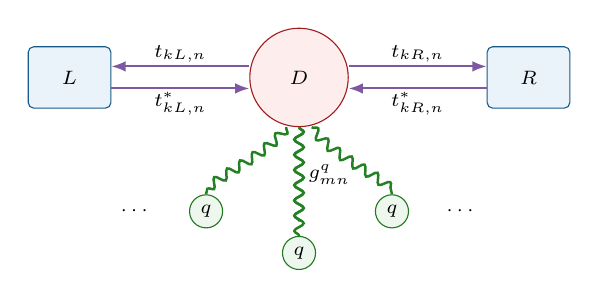
\begin{tikzpicture}[baseline=(D.base),font=\scriptsize]
  \tikzset{
    phline/.style={
      draw=phononcolor!80!black,
      line width=0.9pt,
      decorate,
      decoration={snake,amplitude=1.7pt,segment length=5.5pt}
    }
  }

  % --- Main electronic regions ---
  \node[
    devbox,
    minimum width=1.05cm,
    minimum height=0.78cm,
    fill=leadbg,
    draw=leadcolor!75!black
  ] (L) {$L$};

  \node[
    devdot,
    minimum size=1.25cm,
    fill=fermionbg,
    draw=fermioncolor!75!black,
    right=1.75cm of L
  ] (D) {$D$};

  \node[
    devbox,
    minimum width=1.05cm,
    minimum height=0.78cm,
    fill=leadbg,
    draw=leadcolor!75!black,
    right=1.75cm of D
  ] (R) {$R$};

  % --- L-D tunneling ---
  \draw[hoparrow,draw=hopcolor!85!black]
    ($(D.west)+(0,0.14)$) --
    node[above,fill=white,inner sep=1pt] {$t_{kL,n}$}
    ($(L.east)+(0,0.14)$);

  \draw[hoparrow,draw=hopcolor!85!black]
    ($(L.east)+(0,-0.14)$) --
    node[below,fill=white,inner sep=1pt] {$t_{kL,n}^{*}$}
    ($(D.west)+(0,-0.14)$);

  % --- D-R tunneling ---
  \draw[hoparrow,draw=hopcolor!85!black]
    ($(D.east)+(0,0.14)$) --
    node[above,fill=white,inner sep=1pt] {$t_{kR,n}$}
    ($(R.west)+(0,0.14)$);

  \draw[hoparrow,draw=hopcolor!85!black]
    ($(R.west)+(0,-0.14)$) --
    node[below,fill=white,inner sep=1pt] {$t_{kR,n}^{*}$}
    ($(D.east)+(0,-0.14)$);

  % --- Phonon sector ---
  \node[
    draw=phononcolor!75!black,
    fill=phononbg,
    circle,
    minimum size=0.42cm,
    below left=1.10cm and 0.58cm of D,
    inner sep=0pt
  ] (q1) {$q$};

  \node[
    draw=phononcolor!75!black,
    fill=phononbg,
    circle,
    minimum size=0.42cm,
    below=1.38cm of D,
    inner sep=0pt
  ] (q2) {$q$};

  \node[
    draw=phononcolor!75!black,
    fill=phononbg,
    circle,
    minimum size=0.42cm,
    below right=1.10cm and 0.58cm of D,
    inner sep=0pt
  ] (q3) {$q$};

  % --- Ellipses to indicate many phonon modes ---
  \node[left=0.35cm of q1,font=\scriptsize] {$\cdots$};
  \node[right=0.35cm of q3,font=\scriptsize] {$\cdots$};

  % --- Electron-phonon coupling ---
  \draw[phline]
    (D.south) --
    node[right=2pt,fill=white,inner sep=1pt] {$g_{mn}^{q}$}
    ($(q2.north)+(0,0.18)$);

  \draw[phline]
    ($(D.south)+(-0.16,0)$)
    .. controls +(-0.30,-0.40) and +(0,0.22) ..
    (q1.north);

  \draw[phline]
    (D.south)
    .. controls +(0,-0.45) and +(0,0.22) ..
    (q2.north);

  \draw[phline]
    ($(D.south)+(0.16,0)$)
    .. controls +(0.30,-0.40) and +(0,0.22) ..
    (q3.north);

\end{tikzpicture}%
}
\caption{
Schematic of the lead-device-lead geometry with phonons. The central interacting region $D$
is coupled to the left and right reservoirs through tunneling amplitudes
$t_{k\alpha,n}$ and to phonon modes through matrix-valued
electron-phonon couplings $g_{mn}^{q}$. The reservoirs enter through their
embedding self-energies, while the electron-phonon interaction is confined
to $D$.
}
\label{fig:ldl-schematic}
\end{figure}


\subsection{Hamiltonian}

\begin{center}
\begin{adjustbox}{max width=\linewidth,max totalheight=0.82\textheight,keepaspectratio}
$\displaystyle H = \hamterm{leadcolor}{leadbg}{\sum_{k\alpha} \epsilon_{k\alpha}(t) c_{k\alpha}^{\dagger} c_{k\alpha}} + \hamterm{fermioncolor}{fermionbg}{\sum_{mn} \epsilon_{mn}(t) d_m^{\dagger} d_n}$
\end{adjustbox}
\end{center}
\begin{center}
\begin{adjustbox}{max width=\linewidth,max totalheight=0.82\textheight,keepaspectratio}
$\displaystyle + \hamterm{hopcolor}{hopbg}{\sum_{k\alpha,n} (t_{k\alpha,n} c_{k\alpha}^{\dagger} d_n + t_{k\alpha,n}^{*} d_n^{\dagger} c_{k\alpha})}$
\end{adjustbox}
\end{center}
\begin{center}
\begin{adjustbox}{max width=\linewidth,max totalheight=0.82\textheight,keepaspectratio}
$\displaystyle + \hamterm{phononcolor}{phononbg}{\sum_q \omega_q \left(b_q^{\dagger} b_q + \frac{1}{2}\right)} + \hamterm{elphcolor}{elphbg}{\sum_{mn,q} g_{mn}^q d_m^{\dagger} d_n (b_q^{\dagger} + b_q)}$
\end{adjustbox}
\end{center}
Here \(c_{k\alpha}^{\dagger}\) (\(c_{k\alpha}\)), with
\(\alpha=L,R\), creates (annihilates) an electron in lead state \(k\),
\(d_n^{\dagger}\) (\(d_n\)) creates (annihilates) an electron in device
state \(n\), and \(b_q^{\dagger}\) (\(b_q\)) creates (annihilates) a
phonon in mode \(q\) of the central region. The \hamsquare{leadcolor}{leadbg} term describes the isolated leads. The \hamsquare{fermioncolor}{fermionbg} term
describes the fermions in the isolated scattering region. The
\hamsquare{phononcolor}{phononbg} term describes the phonons in the isolated scattering region. More specifically, it describes the finite set of uncoupled quantum harmonic oscillators. The \hamsquare{hopcolor}{hopbg} term describes hopping processes between leads and the scattering region with strength \(t_{k\alpha,n}\).
The \hamsquare{elphcolor}{elphbg} term represents the interaction of the fermions with the phonons, where \(g_{mn}^q\) is the electron-phonon coupling matrix. 

Within the adiabatic-potential approximation, $\epsilon_{k\alpha}(t)=\epsilon_{k\alpha}^0+\Delta_\alpha(t)$ and $\epsilon_{mn}(t)=\epsilon_{mn}^0+\Delta_{mn}(t)$, where the superscript $0$ denotes the stationary reference problem and the $\Delta$'s are prescribed one-body shifts. The lead shift is taken uniform within each reservoir, whereas $\bm\Delta(t)$ may be a matrix in the device basis. This is the same rigid-shift representation used in finite-bandwidth pulse transport: the detailed lead spectrum remains in $\Gamma_\alpha(\epsilon)$, while the external field enters through time-dependent phases. Hermiticity requires $\epsilon_{mn}(t)=\epsilon_{nm}^*(t)$ and $g_{mn}^q=(g_{nm}^q)^*$.



\subsection{Conventions and assumptions}
\label{sec:assumptions}

The lead-device couplings are present at all times; the voltage pulse does not switch on the contacts. To describe this, we use the partition-free formulation developed in Sec.~\ref{sec:partition-free-dyson}, in which the connected electronic system is already present before the drive \cite{Cini1980,StefanucciAlmbladh2004}. We work on the two real-time branches of the Schwinger-Keldysh contour and do not append a Matsubara branch shown in Fig.~\ref{fig:keldysh-contour}.
\begin{figure}[ht]
\centering
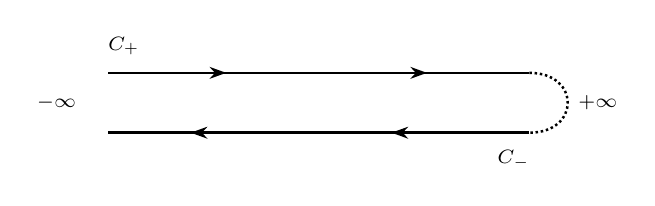
\begin{tikzpicture}[
    x=1cm,
    y=1cm,
    font=\scriptsize,
    >=Stealth,
    branch/.style={draw=black,line width=0.9pt},
    dir/.style={-{Stealth[length=2.1mm,width=1.5mm]},
                draw=black,line width=0.9pt}
]

\coordinate (Lp) at (0.75, 0.38);
\coordinate (Rp) at (6.10, 0.38);
\coordinate (Lm) at (0.75,-0.38);
\coordinate (Rm) at (6.10,-0.38);

\draw[branch] (Lp) -- (Rp);
\draw[branch] (Rm) -- (Lm);

\draw[dir] (1.75,0.38) -- (2.25,0.38);
\draw[dir] (4.30,0.38) -- (4.80,0.38);
\draw[dir] (4.85,-0.38) -- (4.35,-0.38);
\draw[dir] (2.30,-0.38) -- (1.80,-0.38);

\draw[
    draw=black,
    line width=0.9pt,
    densely dotted
]
(Rp)
.. controls +(0.65,0) and +(0.65,0) ..
(Rm);

\node[above=0.10cm] at (0.95,0.38) {$C_+$};
\node[below=0.10cm] at (5.90,-0.38) {$C_-$};
\node[left=0.28cm] at ($(Lp)!0.5!(Lm)$) {$-\infty$};
\node[right=0.50cm] at ($(Rp)!0.5!(Rm)$) {$+\infty$};

\end{tikzpicture}
\caption{
Closed two-branch Schwinger-Keldysh contour. The contour evolves from $-\infty$ to $+\infty$ along \(C_+\) and returns to $-\infty$ along \(C_-\).}
\label{fig:keldysh-contour}
\end{figure}
The term \emph{unbiased} refers only to the absence of an applied voltage difference. The phonon propagators are prescribed equilibrium thermal functions \(\widetilde D_q(t-t')\) with frequencies \(\omega_q\) and Bose occupations \(N_q=f_b(\omega_q)\). Tilded electronic quantities denote equilibrium reference objects without electron-phonon dressing: \(\widetilde G^0\) is the connected zero-pulse electronic propagator and \(\widetilde\Sigma_\alpha\) is the unshifted lead embedding. For a protocol \(p\), \(\bar G_{\mathcal P,p}\equiv\proj_p G_p\) denotes the projected stationary electronic feedback propagator. The corresponding projected interaction self-energy is denoted \(\barSigma_{\rm ep,p}\). Undecorated quantities carry the full explicit two-time dependence generated by the voltage protocol.

The externally applied fields are represented by rigid one-body shifts. Following the adiabatic-potential approximation used in finite-bandwidth pulse transport \cite{JauhoWingreenMeir1994,MaciejkoWangGuo2006}, the lead shift is uniform within each reservoir, whereas the device shift \(\bm\Delta(t)\) may be a matrix in the chosen device basis. The complete energy dependence of the lead linewidth \(\Gamma_\alpha(\epsilon)\) is retained; the wide-band limit is introduced only as a limiting check.

PS-SCBA retains Hartree and Fock electron-phonon diagrams with the prescribed thermal phonon propagator and neglects vertex corrections and phonon backaction. Its additional approximation is temporal: only the projected time-translation-invariant electronic sector is fed back into those diagrams. The complete driven Green function is still computed, and its complementary component is retained for numerical diagnostics to evaluate the impact of this approximation. Causality of the inner Dyson propagation is retained for every fixed stationary kernel.


\subsection{Time-dependent current}
\label{sec:time-current}
The current flowing from lead $\alpha$ is defined by $J_\alpha(t)\equiv-e\langle\dot N_\alpha(t)\rangle$, where $N_\alpha=\sum_k c_{k\alpha}^{\dagger}c_{k\alpha}$ is the particle-number operator of that lead. Using the Heisenberg equation and the mixed lead-device Green function gives
\begin{equation}
J_\alpha(t)
=
2e\,\operatorname{Re}
\sum_{kn}
t_{k\alpha,n}
G_{n,k\alpha}^{<}(t,t),
\label{eq:mixed-current}
\end{equation}
where
\begin{equation*}
G_{n,k\alpha}^{<}(t,t')
=
i\left\langle
c_{k\alpha}^{\dagger}(t')d_n(t)
\right\rangle
\end{equation*}
is the mixed device-lead lesser Green function. To determine this quantity, introduce the corresponding contour-ordered Green function
\begin{equation*}
G_{n,k\alpha}(\tau,\tau')
=
-i
\left\langle
T_C
d_n(\tau)c_{k\alpha}^{\dagger}(\tau')
\right\rangle,
\end{equation*}
with \(\tau,\tau'\in C\). We use the closed two-branch Schwinger-Keldysh contour.

\subsection{Perturbation expansion of the mixed Green function}
\label{subsec:mixed-expansion}

We now derive the contour equation for the mixed Green function. We follow the procedure in \cite{Haug2008}. We start by splitting the Hamiltonian as
\begin{equation*}
H=H_0+V,
\end{equation*}
with
\begin{align*}
H_0(t)
={}&
\sum_{k\alpha}
\epsilon_{k\alpha}(t)
c_{k\alpha}^{\dagger}c_{k\alpha}
+
\sum_{mn}
\epsilon_{mn}(t)
d_m^{\dagger}d_n
\\
&+
\sum_q
\omega_q
\left(
b_q^{\dagger}b_q+\frac{1}{2}
\right),
\end{align*}
and
\begin{equation*}
V=V_T+V_{\rm ep}.
\end{equation*}
The tunnelling interaction is
\begin{equation*}
V_T
=
\sum_{k\alpha,n}
\left(
t_{k\alpha,n}
c_{k\alpha}^{\dagger}d_n
+
t_{k\alpha,n}^{*}
d_n^{\dagger}c_{k\alpha}
\right),
\end{equation*}
while the electron-phonon interaction is
\begin{equation*}
V_{\rm ep}
=
\sum_{mnq}
g_{mn}^{q}
d_m^{\dagger}d_nX_q,
\end{equation*}
where
\begin{equation*}
X_q=b_q+b_q^{\dagger}.
\end{equation*}
The averages associated with \(H_0\) define the isolated central-region propagator
\begin{equation*}
G_{nm}^{(0)}(\tau,\tau')
=
-i
\left\langle
T_C d_n(\tau)d_m^{\dagger}(\tau')
\right\rangle_0,
\end{equation*}
the isolated lead propagator
\begin{equation*}
g_{k\alpha}(\tau,\tau')
=
-i
\left\langle
T_C c_{k\alpha}(\tau)c_{k\alpha}^{\dagger}(\tau')
\right\rangle_0,
\end{equation*}
and the equilibrium phonon propagator
\begin{equation*}
\widetilde D_{qq'}(\tau,\tau')
=
-i
\left\langle
T_C X_q(\tau)X_{q'}(\tau')
\right\rangle_0
=
\delta_{qq'}\widetilde D_q(\tau,\tau').
\end{equation*}
The interacting central-region Green function is
\begin{equation}
G_{nm}(\tau,\tau')
=
-i
\left\langle
T_C d_n(\tau)d_m^{\dagger}(\tau')
\right\rangle.
\label{eq:central-G-def}
\end{equation}
The contour evolution operator is
\begin{equation*}
\mathcal S_C
=
T_C
\exp\!\left[
-i\oint_C d\tau\,V_I(\tau)
\right],
\end{equation*}
so that the mixed Green function
\begin{equation*}
G_{n,k\alpha}(\tau,\tau')
=
-i
\left\langle
T_C\{\mathcal S_C
d_n(\tau)c_{k\alpha}^{\dagger}(\tau')
\}\right\rangle,
\end{equation*}
has the Keldysh perturbation series
\begin{align*}
G_{n,k\alpha}(\tau,\tau')
={}&
\sum_{\ell=0}^{\infty}
\frac{(-i)^{\ell+1}}{\ell!}
\oint_C d\tau_1\cdots d\tau_\ell
\\
&\times
\left\langle
T_C
d_n(\tau)
V_I(\tau_1)\cdots V_I(\tau_\ell)
c_{k\alpha}^{\dagger}(\tau')
\right\rangle_0 .
\end{align*}
The zeroth-order contribution vanishes because the lead and central-region fields are uncoupled in \(H_0\). The leading nonzero term contains one tunnelling vertex,
\begin{equation*}
G_{n,k\alpha}^{(1)}(\tau,\tau')
=
\sum_m
\oint_C d\tau_1\,
G_{nm}^{(0)}(\tau,\tau_1)
t_{k\alpha,m}^{*}
g_{k\alpha}(\tau_1,\tau').
\end{equation*}
Its contraction is shown in Fig.~\ref{fig:mixed-leading}.
\begin{figure}[ht]
\centering
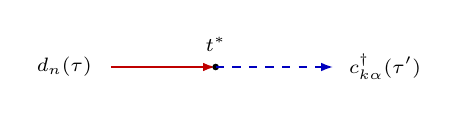
\begin{tikzpicture}[
    x=1.0cm,
    y=1.0cm,
    fermionline/.style={
        draw=red!75!black,
        line width=0.9pt,
        -{Latex[length=1.6mm,width=1.1mm]}
    },
    leadline/.style={
        draw=blue!75!black,
        dashed,
        line width=0.9pt,
        -{Latex[length=1.6mm,width=1.1mm]}
    }
]

\node[font=\scriptsize,anchor=east] at (0,0)
{$d_n(\tau)$};

\draw[fermionline] (0.12,0) -- (1.45,0);
\fill (1.45,0) circle (1.2pt);
\draw[leadline] (1.45,0) -- (2.95,0);

\node[font=\scriptsize,above=2pt] at (1.45,0)
{$t^{*}$};

\node[font=\scriptsize,anchor=west] at (3.02,0)
{$c_{k\alpha}^{\dagger}(\tau')$};

\end{tikzpicture}
\caption{
Leading contribution to the mixed Green function. The solid red line denotes a central-region electron propagator and the dashed blue line denotes an isolated lead propagator.}
\label{fig:mixed-leading}
\end{figure}
There is no contribution at second order. Two tunnelling vertices leave an odd number of lead fields. A tunnelling vertex together with one electron-phonon vertex leaves a single displacement \(X_q\) unpaired, while two electron-phonon vertices leave the external lead operator unpaired. The first contribution involving phonons therefore occurs at third order. Since $\left\langle X_q(\tau)\right\rangle_0=0$, two electron-phonon vertices are required to form a phonon contraction, together with one tunnelling vertex to connect the external lead operator. The nonvanishing connected third-order classes are therefore $V_TV_TV_T$, and $V_TV_{\rm ep}V_{\rm ep}$. The first class generates the next lead insertion in the central-region propagator. The second class contains the exchange and tadpole contractions shown in
Fig.~\ref{fig:mixed-ep-topologies}.
\begin{figure}[ht]
\centering
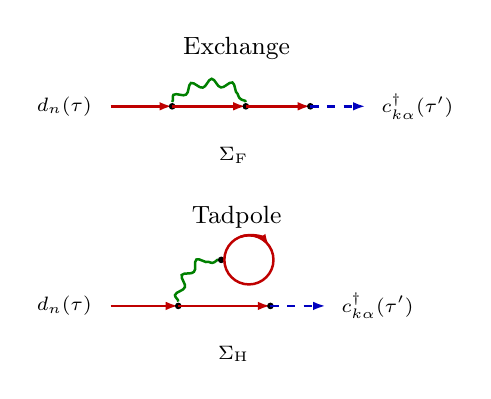
\begin{tikzpicture}[
    x=0.78cm,
    y=0.78cm,
    fermionline/.style={
        draw=red!75!black,
        line width=0.9pt,
        -{Latex[length=1.6mm,width=1.1mm]}
    },
    leadline/.style={
        draw=blue!75!black,
        dashed,
        line width=0.9pt,
        -{Latex[length=1.6mm,width=1.1mm]}
    },
    phononline/.style={
        draw=green!50!black,
        line width=0.9pt,
        decorate,
        decoration={snake,amplitude=0.50mm,segment length=2.5mm}
    }
]

% Exchange
\node[font=\small] at (2.15,1.20) {Exchange};

\node[font=\scriptsize,anchor=east] at (-0.05,0.25)
{$d_n(\tau)$};

\draw[fermionline] (0.10,0.25) -- (1.10,0.25);
\fill (1.10,0.25) circle (1.2pt);

\draw[fermionline] (1.10,0.25) -- (2.30,0.25);
\fill (2.30,0.25) circle (1.2pt);

\draw[fermionline] (2.30,0.25) -- (3.35,0.25);
\fill (3.35,0.25) circle (1.2pt);

\draw[leadline] (3.35,0.25) -- (4.25,0.25);

\node[font=\scriptsize,anchor=west] at (4.35,0.25)
{$c_{k\alpha}^{\dagger}(\tau')$};

\draw[phononline] (1.10,0.32) to[bend left=47] (2.30,0.32);

\node[font=\scriptsize] at (2.10,-0.55)
{$\Sigma_{\rm F}$};

% Tadpole
\node[font=\small] at (2.15,-1.55) {Tadpole};

\node[font=\scriptsize,anchor=east] at (-0.05,-3.00)
{$d_n(\tau)$};

\draw[fermionline] (0.10,-3.00) -- (1.20,-3.00);
\fill (1.20,-3.00) circle (1.2pt);

\draw[fermionline] (1.20,-3.00) -- (2.70,-3.00);
\fill (2.70,-3.00) circle (1.2pt);

\draw[leadline] (2.70,-3.00) -- (3.60,-3.00);

\node[font=\scriptsize,anchor=west] at (3.70,-3.00)
{$c_{k\alpha}^{\dagger}(\tau')$};

\draw[phononline]
(1.20,-2.93)
to[bend left=40]
(1.90,-2.25);

\fill (1.90,-2.25) circle (1.2pt);

\draw[
    draw=red!75!black,
    line width=0.9pt
]
(2.35,-2.25) circle[radius=0.40];

\draw[
    draw=red!75!black,
    line width=0.9pt,
    -{Latex[length=1.5mm,width=1.0mm]}
]
($(2.35,-2.25)+(110:0.40)$)
arc[start angle=110,end angle=35,radius=0.40];

\node[font=\scriptsize] at (2.10,-3.78)
{$\Sigma_{\rm H}$};

\end{tikzpicture}
\caption{
Connected electron-phonon contributions to the mixed Green function at third order. Solid red lines denote central-region electron propagators, dashed blue lines denote lead propagators, and wavy green lines denote equilibrium phonon propagators. The exchange topology generates the Fock contribution, while the tadpole topology generates the Hartree contribution.}
\label{fig:mixed-ep-topologies}
\end{figure}
The exchange and tadpole contractions are the same two electron-phonon structures that enter the central-region self-energy. Disconnected vacuum contributions cancel through the normalization of the contour expectation value. Collecting the connected terms gives, schematically,
\begin{equation*}
G^{(0)}
+
G^{(0)}\Sigma^{\rm lead}G^{(0)}
+
G^{(0)}\Sigma_{\rm ep}G^{(0)}
+\cdots ,
\end{equation*}
which is the beginning of the perturbation series for the interacting central-region Green function. Resumming the corresponding insertions therefore gives the mixed contour propagator in the compact form
\begin{equation}
G_{n,k\alpha}(\tau,\tau')
=
\sum_m
\oint_C d\tau_1\,
G_{nm}(\tau,\tau_1)
t_{k\alpha,m}^{*}
g_{k\alpha}(\tau_1,\tau').
\label{eq:mixed-contour-final}
\end{equation}
Thus the lead and electron-phonon insertions associated with the central region are contained in \(G\), while the final lead line is described by the isolated propagator  \(g_{k\alpha}\).

\subsection{Analytic Langreth continuation}
\label{subsec:mixed-continuation}

We now project Eq.~\eqref{eq:mixed-contour-final} onto the real-time branches. For a contour convolution \(C=A\circ B\), the Langreth rules give
\begin{equation*}
C^< = A^R\!\cdot B^< + A^<\!\cdot B^A,
\qquad
C^R = A^R\!\cdot B^R,
\end{equation*}
where the dot denotes real-time integration. Applying the lesser projection to Eq.~\eqref{eq:mixed-contour-final} gives
\begin{equation}
\begin{aligned}
G_{n,k\alpha}^{<}(t,t')
={}&
\sum_m
\int_{-\infty}^{\infty}dt_1\,
t_{k\alpha,m}^{*}\Big[
G_{nm}^{R}(t,t_1)
g_{k\alpha}^{<}(t_1,t')
\\
&\qquad+
G_{nm}^{<}(t,t_1)
g_{k\alpha}^{A}(t_1,t')
\Big].
\end{aligned}
\label{eq:mixed-lesser-langreth}
\end{equation}
For $\epsilon_{k\alpha}(t) = \epsilon_{k\alpha}^{0} + \Delta_\alpha(t),$ the isolated lead propagators are
\begin{equation*}
g_{k\alpha}^{<}(t,t')
=
i f(\epsilon_{k\alpha}^{0})
\exp\!\left[
-i\int_{t'}^{t}du\,
\epsilon_{k\alpha}(u)
\right],
\end{equation*}
and
\begin{equation*}
g_{k\alpha}^{R,A}(t,t')
=
\mp i
\Theta[\pm(t-t')]
\exp\!\left[
-i\int_{t'}^{t}du\,
\epsilon_{k\alpha}(u)
\right].
\end{equation*}
Here \(f(\epsilon)\) is the Fermi distribution of the lead. It is convenient to introduce the energy-dependent linewidth matrix
\begin{equation*}
\Gamma_{\alpha,mn}(\epsilon)
=
2\pi
\sum_k
t_{k\alpha,m}^{*}
t_{k\alpha,n}
\delta(\epsilon-\epsilon_{k\alpha}^{0}).
\end{equation*}
Substitution of Eq.~\eqref{eq:mixed-lesser-langreth} into Eq.~\eqref{eq:mixed-current}, followed by the sum over lead states, gives
\begin{equation}
\boxed{
\begin{aligned}
J_\alpha(t)
={}&
-2e
\int_{-\infty}^{t}dt'
\int\frac{d\epsilon}{2\pi}\,
\operatorname{Im}
\operatorname{Tr}
\Bigg\{
e^{i\epsilon(t-t')}
\\
&\times
e^{i\int_{t'}^{t}du\,\Delta_\alpha(u)}
\Gamma_\alpha(\epsilon)
\Big[
G^<(t,t')\\
&\qquad+
f(\epsilon)G^R(t,t')
\Big]
\Bigg\}.
\label{eq:current-reduced}
\end{aligned}}
\end{equation}
Equation~\eqref{eq:current-reduced} expresses the time-dependent current entirely in terms of the central-region retarded and lesser Green functions. Its structure is the same as in the finite-bandwidth partition-free formulation of Maciejko \textit{et al.} \cite{MaciejkoWangGuo2006}, with the interacting central-region propagators generated by the resummation of the electronic self-energies in the spirit of the Meir-Wingreen construction
\cite{MeirWingreen1992}.

For the subsequent time-dependent analysis, it is convenient to collect the time convolutions entering the current into auxiliary functions. We first define
\begin{align}
A_{\alpha,mn}(\epsilon,t)
\equiv{}&
\int_{-\infty}^{t}dt'\,
e^{i\epsilon(t-t')}
\notag\\
&\times
\exp\!\left[
i\int_{t'}^{t}du\,\Delta_\alpha(u)
\right]
G_{mn}^{R}(t,t'),
\label{eq:Aalpha-definition}
\end{align}
and, analogously,
\begin{align}
\Psi_{\alpha,mn}(\epsilon,t)
\equiv{}&
\int_{-\infty}^{t}dt'\,
e^{i\epsilon(t-t')}
\notag\\
&\times
\exp\!\left[
i\int_{t'}^{t}du\,\Delta_\alpha(u)
\right]
G_{mn}^{<}(t,t').
\label{eq:Psi-definition}
\end{align}
Both \(A_\alpha\) and \(\Psi_\alpha\) are matrices in the central-region single-particle indices. The lead-dependent phase accounts for the time-dependent shift \(\Delta_\alpha(t)\), while the central-region dynamics are carried by \(G^R\) and \(G^<\). A second retarded auxiliary function will also be required below when the electron-phonon contribution to the lesser Green function is evaluated. We define
\begin{align}
C_{mn}(t,\omega,\epsilon')
\equiv{}&
\int_{-\infty}^{t}dt'\,
G_{mn}^{R}(t,t')
e^{i(\omega+\epsilon')(t-t')}.
\end{align}
Here \(\omega\) is an auxiliary energy argument. In the electron-phonon contribution it is evaluated at the phonon-mode frequencies, $\omega=\pm\omega_q$, where \(q\) labels the phonon modes and \(\omega_q\) is the frequency of mode \(q\). 

Finally, it is useful to separate the current according to its retarded and lesser contributions,
\begin{equation*}
J_\alpha(t)
=
J_\alpha^{R}(t)
+
J_\alpha^{<}(t).
\end{equation*}
From Eq.~\eqref{eq:current-reduced}, the retarded contribution is
\begin{equation*}
J_\alpha^{R}(t)
=
-2e
\int_{-\infty}^{\infty}
\frac{d\epsilon}{2\pi}\,
f(\epsilon)
\operatorname{Im}
\operatorname{Tr}
\left[
\Gamma_\alpha(\epsilon)
A_\alpha(\epsilon,t)
\right],
\end{equation*}
whereas the lesser contribution is
\begin{equation*}
J_\alpha^{<}(t)
=
-2e
\int_{-\infty}^{\infty}
\frac{d\epsilon}{2\pi}\,
\operatorname{Im}
\operatorname{Tr}
\left[
\Gamma_\alpha(\epsilon)
\Psi_\alpha(\epsilon,t)
\right].
\end{equation*}
The current can therefore be written compactly as
\begin{equation}
\boxed{
\begin{aligned}
J_\alpha(t)
={}&
-2e
\int_{-\infty}^{\infty}
\frac{d\epsilon}{2\pi}\,
\operatorname{Im}
\operatorname{Tr}
\Big\{
\Gamma_\alpha(\epsilon)
\\
&\qquad\times
\left[
\Psi_\alpha(\epsilon,t)
+
f(\epsilon)A_\alpha(\epsilon,t)
\right]
\Big\}.
\end{aligned}}
\label{eq:Jalpha-A-Psi}
\end{equation}

The auxiliary functions \(A_\alpha\), \(\Psi_\alpha\), and \(C\) will be evaluated for the voltage protocols considered below. The retarded dynamics determine both \(A_\alpha\) and \(C\), while the lesser dynamics enter through \(\Psi_\alpha\). Their explicit construction follows from the partition-free Dyson equation derived in Sec.~\ref{sec:partition-free-dyson}. The role of \(C\) becomes explicit when the electron-phonon contribution to \(\Psi_\alpha\) is developed.

\section{Partition-Free Dyson Equation}
\label{sec:partition-free-dyson}

The current expressions derived above reduce the transport problem to the determination of the central-region Green functions \(G^R\) and
\(G^<\). We now construct these quantities in the partition-free formulation. The leads and central region are already coupled in the initial stationary preparation, while the subsequent voltage protocol is treated as a time-dependent perturbation of the connected system. The derivation is carried out on the same closed two-branch Keldysh contour \(C=C_+\cup C_-\) introduced above.

The main point is to separate the stationary connected system from the explicit pulse dependence while retaining the electron-phonon interaction in the central region. We first remove the time-dependent lead energies by a gauge transformation, integrate out the lead and equilibrium phonon fields, and then derive the interacting partition-free Dyson equation by means of the electronic generating functional.

\subsection{Gauge transformation of the lead voltage}
\label{subsec:pf-gauge}

The lead energies have the form
\begin{equation*}
\epsilon_{k\alpha}(t)
=
\epsilon_{k\alpha}^{0}
+
\Delta_\alpha(t).
\end{equation*}
Introduce the accumulated phase
\begin{equation*}
\Phi_\alpha(t)
=
\int_{0}^{t}ds\,\Delta_\alpha(s),
\end{equation*}
and the unitary transformation
\begin{equation*}
\mathcal U(t)
=
\exp\!\left[
i\sum_{k\alpha}
\Phi_\alpha(t)c_{k\alpha}^{\dagger}c_{k\alpha}
\right].
\end{equation*}
Since
\begin{equation*}
\mathcal U c_{k\alpha}\mathcal U^\dagger
=
e^{-i\Phi_\alpha(t)}c_{k\alpha},
\qquad
\mathcal U c_{k\alpha}^{\dagger}\mathcal U^\dagger
=
e^{i\Phi_\alpha(t)}c_{k\alpha}^{\dagger},
\end{equation*}
while the central electron and phonon operators are unchanged, the transformed Hamiltonian
\begin{equation*}
\widehat H(t)
=
\mathcal U H(t)\mathcal U^\dagger
+
i\dot{\mathcal U}\mathcal U^\dagger
\end{equation*}
contains the stationary lead energies \(\epsilon_{k\alpha}^{0}\).
Indeed,
\begin{equation*}
i\dot{\mathcal U}\mathcal U^\dagger
=
-\sum_{k\alpha}
\Delta_\alpha(t)c_{k\alpha}^{\dagger}c_{k\alpha},
\end{equation*}
which cancels the explicit lead-energy shift. The transformed Hamiltonian is therefore
\begin{align}
\widehat H(t)
={}&
\sum_{k\alpha}
\epsilon_{k\alpha}^{0}
c_{k\alpha}^{\dagger}c_{k\alpha}
+
\sum_{mn}
\epsilon_{mn}(t)d_m^{\dagger}d_n
\notag\\
&+
\sum_{k\alpha n}
\left[
t_{k\alpha,n}(t)c_{k\alpha}^{\dagger}d_n
+
t_{k\alpha,n}^{*}(t)d_n^{\dagger}c_{k\alpha}
\right]
\notag\\
&+
\sum_q
\omega_q
\left(
b_q^{\dagger}b_q+\frac12
\right)
+
\sum_{mnq}
g_{mn}^{q}
d_m^{\dagger}d_n
X_q ,
\label{eq:transformed-Hamiltonian}
\end{align}
where
\begin{equation}
t_{k\alpha,n}(t)
=
e^{i\Phi_\alpha(t)}t_{k\alpha,n},
\qquad
t_{k\alpha,n}^{*}(t)
=
e^{-i\Phi_\alpha(t)}t_{k\alpha,n}^{*}.
\label{eq:pf-hopping-phase}
\end{equation}
Thus the voltage dependence of lead \(\alpha\) has been transferred entirely from its single-particle energies to the tunnelling phases.

\subsection{Keldysh functional integral}
\label{subsec:pf-functional}

On the contour \(C\), the electronic variables \(c,\bar c,d,\bar d\) are Grassmann fields and the phonon variables \(b,\bar b\) are complex commuting fields. We write
\begin{equation*}
\epsilon_{mn}(\tau)
=
\epsilon_{mn}^{0}
+
\Delta_{mn}(\tau),
\end{equation*}
where \(\Delta_{mn}(\tau)\) denotes a possible one-body perturbation of the central region. It may be set to zero when the external drive acts only on the leads.

The contour Lagrangian corresponding to Eq.~\eqref{eq:transformed-Hamiltonian} is
\begin{align*}
\mathcal L
={}&
\sum_{k\alpha}
\bar c_{k\alpha}
(i\partial_\tau-\epsilon_{k\alpha}^{0})
c_{k\alpha}
\\
&+
\sum_{mn}
\bar d_m
\left[
(i\partial_\tau)\delta_{mn}
-\epsilon_{mn}^{0}
-\Delta_{mn}(\tau)
\right]
d_n
\\
&+
\sum_q
\bar b_q(i\partial_\tau-\omega_q)b_q
\\
&-
\sum_{k\alpha n}
\left[
\bar c_{k\alpha}
t_{k\alpha,n}(\tau)d_n
+
\bar d_n
t_{k\alpha,n}^{*}(\tau)c_{k\alpha}
\right]
\\
&-
\sum_{mnq}
g_{mn}^{q}\bar d_m d_n
(b_q+\bar b_q).
\end{align*}

To generate the central-region Green functions, introduce Grassmann sources \(\eta_n,\bar\eta_n\) coupled only to the \(d\) fields,
\begin{equation*}
\begin{aligned}
Z[\bar\eta,\eta]
={}&
\mathcal N
\int
\mathcal D[\bar c,c]\,
\mathcal D[\bar d,d]\,
\mathcal D[\bar b,b]
\\
&\times
\exp\Bigg\{
iS
+
i\oint_C d\tau
\sum_n
\Big[
\bar\eta_n(\tau)d_n(\tau)
\\
&\hspace{3cm}
+
\bar d_n(\tau)\eta_n(\tau)
\Big]
\Bigg\}.
\end{aligned}
\end{equation*}
with
\begin{equation*}
S=\oint_C d\tau\,\mathcal L,
\end{equation*}
and normalization chosen such that \(Z[0,0]=1\). The central contour Green function defined in Eq.~\eqref{eq:central-G-def} is generated according to
\begin{equation*}
iG_{nm}(\tau,\tau')
=
\left.
\frac{\delta^2 Z[\bar\eta,\eta]}
{\delta\bar\eta_n(\tau)\,
 \delta\eta_m(\tau')}
\right|_{\eta=\bar\eta=0}.
\end{equation*}

\subsection{Integration over the lead fields}
\label{subsec:pf-integrate-leads}

In the transformed frame the isolated leads are stationary. Define their inverse contour Green operator by
\begin{equation*}
\widehat g_{k\alpha}^{-1}(\tau,\tau')
=
\left(
i\partial_\tau-\epsilon_{k\alpha}^{0}
\right)
\delta_C(\tau,\tau'),
\end{equation*}
with
\begin{equation*}
\oint_C ds\,
\widehat g_{k\alpha}^{-1}(\tau,s)
\widehat g_{k\alpha}(s,\tau')
=
\delta_C(\tau,\tau').
\end{equation*}
The lead fields can be integrated out exactly by the translations
\begin{align*}
c_{k\alpha}(\tau)
={}&
c'_{k\alpha}(\tau)
+
\oint_C d\tau_1\,
\widehat g_{k\alpha}(\tau,\tau_1)
\sum_n
t_{k\alpha,n}(\tau_1)d_n(\tau_1),
\\
\bar c_{k\alpha}(\tau)
={}&
\bar c'_{k\alpha}(\tau)
+
\oint_C d\tau_1\,
\sum_m
\bar d_m(\tau_1)t_{k\alpha,m}^{*}(\tau_1)
\widehat g_{k\alpha}(\tau_1,\tau).
\end{align*}
The shifted lead fields are therefore completely decoupled. Their integration produces the lead self-energy
\begin{equation*}
\Sigma_{mn}^{\rm lead}(\tau,\tau')
=
\sum_{k\alpha}
t_{k\alpha,m}^{*}(\tau)
\widehat g_{k\alpha}(\tau,\tau')
t_{k\alpha,n}(\tau').
\end{equation*}

After the lead fields have been eliminated, the remaining action is
\begin{align*}
S_{d+b}^{\rm eff}
={}&
\oint_C d\tau d\tau'
\sum_{mn}
\bar d_m(\tau)
K_{mn}^{\rm el}(\tau,\tau')
d_n(\tau')
\\
&+
\sum_q
\oint_C d\tau\,
\bar b_q(\tau)
(i\partial_\tau-\omega_q)
b_q(\tau)
\\
&-
\sum_q
\oint_C d\tau\,
\rho_q(\tau)
\left[
b_q(\tau)+\bar b_q(\tau)
\right],
\end{align*}
where
\begin{align*}
K_{mn}^{\rm el}(\tau,\tau')
={}&
g_{0,mn}^{-1}(\tau,\tau')
-\Delta_{mn}(\tau)\delta_C(\tau,\tau')
-
\Sigma_{mn}^{\rm lead}(\tau,\tau'),
\end{align*}
with
\begin{equation*}
g_{0,mn}^{-1}(\tau,\tau')
=
\left[
(i\partial_\tau)\delta_{mn}
-\epsilon_{mn}^{0}
\right]
\delta_C(\tau,\tau'),
\end{equation*}
and
\begin{equation*}
\rho_q(\tau)
=
\sum_{mn}
g_{mn}^{q}
\bar d_m(\tau)d_n(\tau).
\end{equation*}

For real-time arguments, Eq.~\eqref{eq:pf-hopping-phase} gives
\begin{equation*}
\Sigma_{\alpha}^{\rm lead}(t,t')
=
e^{-i[\Phi_\alpha(t)-\Phi_\alpha(t')]}
\widetilde\Sigma_{\alpha}^{\rm lead}(t-t'),
\end{equation*}
where
\begin{equation*}
\widetilde\Sigma_{\alpha,mn}^{\rm lead}(t-t')
=
\sum_k
t_{k\alpha,m}^{*}
\widehat g_{k\alpha}(t-t')
t_{k\alpha,n}
\end{equation*}
is the stationary zero-pulse lead self-energy. Since
\begin{equation*}
\Phi_\alpha(t)-\Phi_\alpha(t')
=
\int_{t'}^{t}ds\,\Delta_\alpha(s),
\end{equation*}
the change of the lead self-energy produced by the pulse is
\begin{align*}
V_{\alpha}^{\rm lead}(t,t')
\equiv{}&
\Sigma_{\alpha}^{\rm lead}(t,t')
-
\widetilde\Sigma_{\alpha}^{\rm lead}(t-t')
\\
={}&
\left[
e^{-i\int_{t'}^{t}ds\,\Delta_\alpha(s)}
-1
\right]
\widetilde\Sigma_{\alpha}^{\rm lead}(t-t').
\end{align*}

\subsection{Integration over the equilibrium phonons}
\label{subsec:pf-integrate-phonons}

We next integrate out the equilibrium harmonic phonon fields. For each mode define
\begin{equation*}
K_q(\tau,\tau')
=
(i\partial_\tau-\omega_q)
\delta_C(\tau,\tau'),
\end{equation*}
and its inverse,
\begin{equation*}
\oint_C ds\,
K_q(\tau,s)
\mathfrak g_q(s,\tau')
=
\delta_C(\tau,\tau').
\end{equation*}
Suppressing contour integrations temporarily, the action of mode \(q\) can be written
\begin{equation*}
S_q
=
\bar b_qK_qb_q
-\rho_qb_q
-\rho_q\bar b_q.
\end{equation*}
Introduce the translations
\begin{equation*}
b_q
=
b'_q+\mathfrak g_q\rho_q,
\qquad
\bar b_q
=
\bar b'_q+\rho_q\mathfrak g_q.
\end{equation*}
Because \(\rho_q\) is Grassmann even, it commutes with the phonon fields, and substitution gives
\begin{equation*}
S_q
=
\bar b'_qK_qb'_q
-
\rho_q\mathfrak g_q\rho_q.
\end{equation*}

Writing the last term explicitly,
\begin{equation*}
\rho_q\mathfrak g_q\rho_q
=
\oint_C d\tau d\tau'\,
\rho_q(\tau)
\mathfrak g_q(\tau,\tau')
\rho_q(\tau').
\end{equation*}
Interchanging the dummy variables \(\tau\leftrightarrow\tau'\) in the same double integral gives
\begin{align*}
\rho_q\mathfrak g_q\rho_q
={}&
\frac12
\oint_C d\tau d\tau'\,
\rho_q(\tau)
\\
&\times
\left[
\mathfrak g_q(\tau,\tau')
+
\mathfrak g_q(\tau',\tau)
\right]
\rho_q(\tau').
\end{align*}
We recall that for the equilibrium displacement \(X_q=b_q+b_q^\dagger\), the quantity in square brackets is the phonon propagator defined previously,
\begin{equation*}
\widetilde D_q(\tau,\tau')
=
-i
\left\langle
T_C X_q(\tau)X_q(\tau')
\right\rangle_0
=
\mathfrak g_q(\tau,\tau')
+
\mathfrak g_q(\tau',\tau).
\end{equation*}
The phonon fields can therefore be integrated out exactly, leaving the electron-only interaction action
\begin{equation}
S_{\rm ep}^{\rm eff}[\bar d,d]
=
-\frac12
\sum_q
\oint_C d\tau d\tau'\,
\rho_q(\tau)
\widetilde D_q(\tau,\tau')
\rho_q(\tau').
\label{eq:Seff-real-time-Keldysh}
\end{equation}
Equivalently,
\begin{align*}
S_{\rm ep}^{\rm eff}
={}&
-\frac12
\sum_q
\sum_{m_1n_1m_2n_2}
g_{m_1n_1}^{q}
g_{m_2n_2}^{q}
\\
&\times
\oint_C d\tau d\tau'\,
\bar d_{m_1}(\tau)d_{n_1}(\tau)
\widetilde D_q(\tau,\tau')
\\
&\times
\bar d_{m_2}(\tau')d_{n_2}(\tau').
\end{align*}
The factor \(1/2\) in
Eq.~\eqref{eq:Seff-real-time-Keldysh} results from symmetrizing the same contour double integral under \(\tau\leftrightarrow\tau'\). It is therefore not an additional diagrammatic symmetry factor.

\subsection{Electronic generating functional and source shift}
\label{subsec:pf-source-shift}

After the lead and phonon fields have been integrated out, define the quadratic electronic generating functional
\begin{equation*}
\begin{aligned}
Z^0[\bar\eta,\eta]
={}&
\mathcal N_0
\int
\mathcal D[\bar d,d]
\exp\Bigg\{
i
\oint_C d\tau d\tau'
\\
&\qquad\times
\sum_{mn} \bar d_m(\tau)
K_{mn}(\tau,\tau')
d_n(\tau')
\\
&\qquad+
i
\oint_C d\tau\,
\Big[
\bar\eta(\tau)d(\tau)
+
\bar d(\tau)\eta(\tau)
\Big]
\Bigg\}.
\end{aligned}
\end{equation*}
where
\begin{align*}
K_{mn}(\tau,\tau')
={}&
g_{0,mn}^{-1}(\tau,\tau')
-\Delta_{mn}(\tau)\delta_C(\tau,\tau')
\\
&-
\Sigma_{mn}^{\rm lead}(\tau,\tau').
\end{align*}
The corresponding no-phonon partition-free electronic propagator is defined by
\begin{equation*}
\sum_r
\oint_C ds\,
K_{mr}(\tau,s)
G_{rn}^{0}(s,\tau')
=
\delta_{mn}\delta_C(\tau,\tau').
\end{equation*}
The notation \(G^0\) is distinct from the bare \(G^{(0)}\) used in the explicit mixed-Green-function expansion. The latter is the isolated central-region propagator before the lead insertions are resummed, whereas \(G^0\) already contains the coupling to the leads and the applied one-body pulse, but no electron-phonon interaction. To evaluate the source dependence of \(Z^0\), define
\begin{align*}
\xi_n(\tau)
&=
\sum_m
\oint_C ds\,
G_{nm}^{0}(\tau,s)\eta_m(s),
\\
\bar\xi_m(\tau)
&=
\sum_n
\oint_C ds\,
\bar\eta_n(s)G_{nm}^{0}(s,\tau).
\end{align*}
and perform the Grassmann translation
\begin{equation}
d=d'-\xi,
\notag\qquad
\bar d=\bar d'-\bar\xi.
\label{eq:d-source-shift}
\end{equation}
The quadratic generating functional therefore becomes
\begin{equation*}
Z^0[\bar\eta,\eta]
=
Z^0[0,0]
\exp\!\left[
-i\bar\eta G^0\eta
\right],
\end{equation*}
where
\begin{equation*}
\bar\eta G^0\eta
\equiv
\oint_C ds\,ds'
\sum_{mn}
\bar\eta_m(s)
G_{mn}^{0}(s,s')
\eta_n(s').
\end{equation*}
The electron-phonon action must, however, be transformed by the same translation. The normalized full generating functional may be written as
\begin{equation}
Z[\bar\eta,\eta]
=
Z^0[\bar\eta,\eta]\,
\frac{
\left\langle
e^{iS_{\rm ep}^{\rm eff}[\bar d,d]}
\right\rangle_{0,\eta}
}{
\left\langle
e^{iS_{\rm ep}^{\rm eff}[\bar d,d]}
\right\rangle_{0,0}
},
\label{eq:full-Z-factorization}
\end{equation}
where \(\langle\cdots\rangle_{0,\eta}\) denotes the normalized quadratic electronic average generated by \(Z^0[\bar\eta,\eta]\). Equation~\eqref{eq:full-Z-factorization} makes explicit that the interaction factor is source dependent and cannot be treated as an independent multiplicative constant.

\subsection{Electron-phonon self-energy}
\label{subsec:pf-ep-self-energy}

Because \(S_{\rm ep}^{\rm eff}\) is second order in the electron-phonon matrix elements,
\begin{equation*}
e^{iS_{\rm ep}^{\rm eff}}
=
1+iS_{\rm ep}^{\rm eff}+O(g^4).
\end{equation*}
Under the source translation Eq.~\eqref{eq:d-source-shift}, the density becomes
\begin{align*}
\rho_q(\tau)
={}&
[\bar d'(\tau)-\bar\xi(\tau)]
g^q
[d'(\tau)-\xi(\tau)]
\\
={}&
\rho'_q(\tau)
-\bar d'(\tau)g^q\xi(\tau)
-\bar\xi(\tau)g^qd'(\tau)
+\bar\xi(\tau)g^q\xi(\tau),
\end{align*}
where
\begin{equation*}
\rho'_q(\tau)
=
\bar d'(\tau)g^qd'(\tau).
\end{equation*}

The terms in \(\rho_q(\tau_1)\rho_q(\tau_2)\) containing exactly one \(\bar\eta\) and one \(\eta\) are
\begin{align*}
\left.
\rho_q(\tau_1)\rho_q(\tau_2)
\right|_{\bar\eta\eta}
={}&
\rho'_q(\tau_1)
\left[
\bar\xi(\tau_2)g^q\xi(\tau_2)
\right]
\\
&+
\left[
\bar\xi(\tau_1)g^q\xi(\tau_1)
\right]
\rho'_q(\tau_2)
\\
&+
\left[
\bar d'(\tau_1)g^q\xi(\tau_1)
\right]
\left[
\bar\xi(\tau_2)g^qd'(\tau_2)
\right]
\\
&+
\left[
\bar\xi(\tau_1)g^qd'(\tau_1)
\right]
\left[
\bar d'(\tau_2)g^q\xi(\tau_2)
\right].
\end{align*}
The first two terms generate the tadpole contraction and the last two generate the exchange contraction shown previously in Fig.~\ref{fig:mixed-ep-topologies}. Interchanging \(\tau_1\leftrightarrow\tau_2\) maps the two members of each pair onto one another, so their multiplicity cancels the explicit factor \(1/2\) in Eq.~\eqref{eq:Seff-real-time-Keldysh}.

The source-independent vacuum contribution cancels against the
normalization in Eq.~\eqref{eq:full-Z-factorization}. The remaining
connected terms give
\begin{equation*}
\begin{aligned}
G_{mn}(\tau,\tau')
={}&
G_{mn}^{0}(\tau,\tau')
+
\sum_{ab}
\oint_C d\tau_1d\tau_2\,
G_{ma}^{0}(\tau,\tau_1)
\\
&\qquad\times
\left[
\Sigma_{\rm ep}^{(2)}
(\tau_1,\tau_2)
\right]_{ab}
G_{bn}^{0}(\tau_2,\tau')
\\
&\qquad\qquad\qquad+
O(g^4).
\end{aligned}
\end{equation*}
with
\begin{equation*}
\Sigma_{\rm ep}^{(2)}
=
\Sigma_{\rm F}^{(2)}
+
\Sigma_{\rm H}^{(2)}.
\end{equation*}
The exchange, or Fock, contribution is
\begin{align*}
\left[
\Sigma_{\rm F}^{(2)}(\tau,\tau')
\right]_{mn}
={}&
i
\sum_{abq}
g_{ma}^{q}
G_{ab}^{0}(\tau,\tau')
\widetilde D_q(\tau,\tau')
g_{bn}^{q},
\end{align*}
while the tadpole, or Hartree, contribution is
\begin{align*}
\left[
\Sigma_{\rm H}^{(2)}(\tau,\tau')
\right]_{mn}
={}&
-i\,
\delta_C(\tau,\tau')
\sum_q
g_{mn}^{q}
\oint_C ds\,
\widetilde D_q(\tau,s)
\\
&\times
\sum_{ab}
g_{ab}^{q}
G_{ba}^{0}(s,s^+).
\end{align*}
Thus $G = G^0 + G^0\Sigma_{\rm ep}^{(2)}G^0 + O(g^4)$. Within the self-consistent Born approximation, the internal electronic propagators in the electron-phonon self-energy are replaced by the dressed propagator \(G\), while the equilibrium phonon propagator \(\widetilde D_q\) is retained. We therefore define
\begin{equation}
\Sigma_{\rm ep}[G]
=
\Sigma_{\rm F}[G]
+
\Sigma_{\rm H}[G],
\label{eq:SCBA-self-energy-total}
\end{equation}
with
\begin{equation}
\left[
\Sigma_{\rm F}[G](\tau,\tau')
\right]_{mn}
=
i
\sum_{abq}
g_{ma}^{q}
G_{ab}(\tau,\tau')
\widetilde D_q(\tau,\tau')
g_{bn}^{q},
\label{eq:SCBA-Fock-contour}
\end{equation}
and
\begin{align}
\left[
\Sigma_{\rm H}[G](\tau,\tau')
\right]_{mn}
={}&
-i\,
\delta_C(\tau,\tau')
\sum_q
g_{mn}^{q}
\oint_C ds\,
\widetilde D_q(\tau,s) \notag
\\
&\times
\sum_{ab}
g_{ab}^{q}
G_{ba}(s,s^+).
\label{eq:SCBA-Hartree-contour}
\end{align}
The corresponding contour Dyson equation is
\begin{equation}
G
=
G^0
+
G^0\Sigma_{\rm ep}[G]G.
\label{eq:scba-dyson-g0}
\end{equation}



\subsection{Projected stationary SCBA closure}
\label{subsec:projected-scba}

The fully self-consistent SCBA equations above are two-time equations under an external pulse. The approximation introduced here is defined directly at the level of the numerical fixed point: the driven Green function is allowed to retain its complete two-time structure inside the pulse solve, but only its time-translation-invariant component is returned to the electron-phonon self-energy in the next outer iteration.

To define this component without imposing periodicity, introduce the real-time Wigner coordinates
\begin{equation*}
T=\frac{t+t'}{2},
\qquad
\tau=t-t'.
\end{equation*}
Let the numerical propagation be defined on a finite time interval
\(\mathcal W=[t_{\min},t_{\max}]\). For a fixed relative time \(\tau\), only center times for which both arguments remain in the numerical interval are admissible,
\begin{equation*}
\mathcal W_\tau
=
\left\{
T:
T+\frac{\tau}{2}\in\mathcal W,\;
T-\frac{\tau}{2}\in\mathcal W
\right\}.
\end{equation*}
Given a non-negative real weight \(w(T)\), define the normalized stationary projector
\begin{equation}
(\proj_{\mathcal W}X)(\tau)
=
\frac{
\displaystyle
\int_{\mathcal W_\tau} dT\,
w(T)
X\!\left(
T+\frac{\tau}{2},
T-\frac{\tau}{2}
\right)
}{
\displaystyle
\int_{\mathcal W_\tau} dT\,w(T)
}.
\label{eq:stationary-projector}
\end{equation}
The complementary component is
\(\qproj_{\mathcal W}=1-\proj_{\mathcal W}\), so that
\begin{equation*}
X(t,t')
=
\bar X_{\mathcal P}(t-t')
+
\delta X(t,t'),
\end{equation*}
where $\bar X_{\mathcal P}=\proj_{\mathcal W}X$, and $\delta X=\qproj_{\mathcal W}X$. On an equally spaced two-time grid, Eq.~\eqref{eq:stationary-projector} is the Toeplitz projection obtained by averaging all entries with the same lag \(i-j\). The finite-window form is used here because a step or a square pulse is not periodic. The projection preserves retarded support, since \(\Theta(t-t')\) is independent of center time, and it preserves the standard lesser Hermiticity relation when \(w(T)\) is real. For a prescribed protocol \(p\), denote by $\mathcal D_p\!\left[\barSigma_{\ep}^{R,<}\right]$ the complete fixed-kernel driven Dyson/Keldysh solve. The PS-SCBA closure is then the outer fixed-point problem
\begin{align}
G_p^{R,<}
&=
\mathcal D_p^{R,<}\!\left[\barSigma_{\ep,p}^{R,<}\right],
\label{eq:psscba-inner-map}
\\
\bar G_{\mathcal P,p}^{R,<}
&=
\proj_p G_p^{R,<},
\label{eq:psscba-project-map}
\\
\barSigma_{\ep,p}^{R,<}
&=
\Sigma_{\ep,\mathrm{SCBA}}^{R,<}
\!\left[\bar G_{\mathcal P,p};\widetilde D\right].
\label{eq:psscba-outer-map}
\end{align}
Equations~\eqref{eq:psscba-inner-map}--\eqref{eq:psscba-outer-map} are the approximation that will be implemented numerically. During one inner solve, \(\barSigma_{\ep,p}^{R,<}(t-t')\) is stationary and fixed, so the retarded pulse equations keep the convolution structure required by the Volterra/Laplace construction. Once that driven trajectory has been evaluated, the stationary component is recomputed and used to update the SCBA kernel. The explicitly nonstationary component \(\qproj_pG_p\) is not fed back, but it is retained as a numerical diagnostic.

The projection is therefore applied \emph{between} complete fixed-kernel pulse solves; it is not a running time-local update during the Volterra propagation. This distinction is essential. A center-time-dependent interaction kernel generated during the inner propagation would remove the stationary convolution structure that makes the analytic step- and square-pulse solver possible. The practical realization of Eqs.~\eqref{eq:psscba-inner-map}--\eqref{eq:psscba-outer-map}, including reconstruction of the projected Green function without storing a dense two-time matrix, is given in Sec.~\ref{sec:dot-code}.

\subsection{Partition-free Dyson equation}
\label{subsec:full-pf-dyson}

The propagator \(G^0\) contains the pulse-dependent lead
self-energy. To expose the partition-free structure explicitly, we
now express it relative to the stationary connected electronic
system before the pulse. Define the zero-pulse propagator
\(\widetilde G^0\) by
\begin{equation*}
\begin{aligned}
(\widetilde G^0)^{-1}
&=
g_0^{-1}
-
\widetilde\Sigma^{\rm lead},
\\
\widetilde\Sigma^{\rm lead}
&=
\sum_\alpha
\widetilde\Sigma_\alpha^{\rm lead}.
\end{aligned}
\end{equation*}

The pulse-driven no-phonon propagator instead satisfies
\begin{equation}
\begin{aligned}
(G^0)^{-1}
&=
g_0^{-1}
-
\Delta
-
\Sigma^{\rm lead}
\\
&=
(\widetilde G^0)^{-1}
-
V_{\rm el},
\end{aligned}
\label{eq:G0-pulse-inverse}
\end{equation}
where
\begin{equation*}
\begin{aligned}
V_{\rm el}(\tau,\tau')
={}&
\Delta(\tau)
\delta_C(\tau,\tau') + V^{\rm lead}(\tau,\tau'),
\end{aligned}
\end{equation*}
and
\begin{equation*}
V^{\rm lead}
=
\Sigma^{\rm lead}
-
\widetilde\Sigma^{\rm lead}.
\end{equation*}
Consequently,
\begin{equation}
\begin{aligned}
G^0
={}&
\widetilde G^0 + \widetilde G^0
V_{\rm el}
G^0.
\end{aligned}
\label{eq:electronic-pf-dyson}
\end{equation}
Combining Eq.~\eqref{eq:G0-pulse-inverse} with the SCBA identity
\begin{equation*}
\begin{aligned}
G^{-1}
={}&
(G^0)^{-1}
-
\Sigma_{\rm ep}[G]
\end{aligned}
\end{equation*}
gives directly
\begin{equation}
\begin{aligned}
G^{-1}
={}&
(\widetilde G^0)^{-1}
-
V_{\rm el}
-
\Sigma_{\rm ep}[G].
\end{aligned}
\label{eq:full-inverse-pf}
\end{equation}

The full partition-free Dyson equation is therefore
\begin{equation}
\begin{aligned}
G_{mn}(\tau,\tau')
={}&
\widetilde G_{mn}^{0}(\tau,\tau')
+
\sum_{m_1n_1}
\oint_C d\tau_1d\tau_2\,
\widetilde G_{m m_1}^{0}
(\tau,\tau_1)
\\
&\qquad\times
V_{m_1n_1}
(\tau_1,\tau_2)
\\
&\qquad\times
G_{n_1n}
(\tau_2,\tau').
\end{aligned}
\label{eq:full-partition-free-phonon-dyson}
\end{equation}
where the contour kernel is
\begin{equation}
\begin{aligned}
V_{mn}(\tau,\tau')
={}&
\Delta_{mn}(\tau)
\delta_C(\tau,\tau')
+
V_{mn}^{\rm lead}(\tau,\tau')
\\
&+
\Sigma_{{\rm ep},mn}[G]
(\tau,\tau').
\end{aligned}
\label{eq:full-V-definition}
\end{equation}
Equation~\eqref{eq:full-partition-free-phonon-dyson} is the formal
partition-free SCBA Dyson equation for the interacting central
region. The equilibrium connected propagator \(\widetilde G^0\) supplies the initial partition-free boundary, \(V^{\rm lead}\) contains the explicit voltage-induced modification of the lead embedding, and \(\Sigma_{\rm ep}[G]\) contains the electron-phonon interaction. Its retarded and lesser projections determine the functions \(G^R\) and \(G^<\) entering Eqs.~\eqref{eq:Aalpha-definition} and \eqref{eq:Psi-definition}. The real-time reduction of this contour equation will be developed next.

Under PS-SCBA, the full interaction functional in Eq.~\eqref{eq:full-V-definition} is replaced inside the driven Dyson equation by the stationary kernel selected by the outer fixed point,
\begin{equation*}
\Sigma_{\ep,\mathrm{SCBA}}^{R,<}
[G_p;\widetilde D](t,t')
\;\longrightarrow\;
\barSigma_{\ep,p}^{R,<}(t-t')
\end{equation*}
where
\begin{equation}
\barSigma_{\ep,p}^{R,<}(t-t')
=
\Sigma_{\ep,\mathrm{SCBA}}^{R,<}
[\proj_pG_p;\widetilde D](t-t').
\label{eq:pf-psscba-replacement}
\end{equation}
This replacement does not set the driven Green function equal to its stationary projection. The full \(G_p(t,t')\) remains in every external Dyson/Keldysh line; only the internal electronic line used to update the SCBA self-energy is projected. For each fixed outer iterate the interaction contribution is therefore a relative-time convolution, enabling the pulse-specific reductions below.



\section{Current driven by an upward step pulse}
\label{sec:up}

Consider the upward-step protocol
\begin{equation*}
\Delta_\alpha(t)=\Delta_\alpha\Theta(t),
\qquad
\bm\Delta(t)=\bm\Delta\Theta(t).
\end{equation*}
For $t<0$ the connected system is in the stationary unbiased SCBA state, and at $t=0$ the lead and device one-body shifts are switched on. In the noninteracting finite-bandwidth problem, the corresponding retarded Dyson equation can be reduced to a causal Volterra equation and solved by the Laplace-transform construction of Maciejko \textit{et al.}~\cite{MaciejkoWangGuo2006}. In the interacting problem this reduction is not available for a fully time-dependent SCBA self-energy.

Indeed, before making the PS-SCBA approximation, the electron-phonon self-energy is a functional of the driven Green function,
\begin{equation*}
\Sigma_{\ep}^{R,<}(t,t')
=
\Sigma_{\ep,\mathrm{SCBA}}^{R,<}
\!\left[G;\widetilde D\right](t,t'),
\end{equation*}
where $\widetilde D$ denotes the stationary thermal phonon propagators. Once the pulse is applied, the driven Green function is no longer time-translation invariant,
\begin{equation*}
G^{R,<}(t,t')\neq G^{R,<}(t-t'),
\end{equation*}
and a fully self-consistent propagation consequently generates
\begin{equation*}
\Sigma_{\ep,\mathrm{SCBA}}^{R,<}
\!\left[G;\widetilde D\right](t,t')
\neq
\Sigma_{\ep,\mathrm{SCBA}}^{R,<}(t-t').
\end{equation*}
The interaction self-energy then carries an independent dependence on both time arguments, so the retarded Dyson integrals no longer form the stationary convolutions required by the Laplace construction. The central approximation of this work is to suppress this pulse-induced functional feedback. During one inner upward solve, \(\barSigma_{\ep}^{\uparrow,R,<}(t-t')\) is stationary and fixed; after the complete two-time \(G^\uparrow(t,t')\) has been obtained, its stationary projection is recomputed and the outer SCBA iteration is continued.

Because the interaction kernel entering each inner solve depends only on a relative time,
\begin{equation*}
\barSigma_{\ep}^{R,<}(t-t')
=
\int\frac{d\omega}{2\pi}
e^{-i\omega(t-t')}
\barSigma_{\ep}^{R,<}(\omega),
\end{equation*}
the projected closure retains the complete frequency dependence, inelastic structure, dispersive part, and lifetime broadening of the current SCBA iterate. The explicit loss of time-translation invariance remains in the driven Green function and in the prescribed voltage-dependent one-body kernels, while the interaction feedback returned to the next SCBA iterate is stationary. For the stationary kernel \(\barSigma_{\ep}^{\uparrow}\), define the unbiased and biased stationary endpoint propagators
\begin{equation*}
\begin{aligned}
\overline G_{\mathrm u}^{\uparrow,R}(z)
={}&
\widetilde G^{0,R}(z)
+
\widetilde G^{0,R}(z)
\barSigma_{\ep}^{R}(z)
\overline G_{\mathrm u}^{\uparrow,R}(z),
\end{aligned}
\end{equation*}
and
\begin{equation*}
\begin{aligned}
\overline G_{\mathrm b}^{\uparrow,R}(z)
={}&
\widetilde G^{0,R}(z)
+
\widetilde G^{0,R}(z)
\Bigg\{
\bm\Delta
+
\barSigma_{\ep}^{R}(z)
\\
&\qquad+
\sum_\beta
\left[
\widetilde\Sigma_\beta^R(z-\Delta_\beta)
-
\widetilde\Sigma_\beta^R(z)
\right]
\Bigg\}
\overline G_{\mathrm b}^{\uparrow,R}(z).
\end{aligned}
\end{equation*}
These are endpoint propagators generated with the same upward protocol-conditioned kernel; neither should be identified with the projected feedback propagator \(\bar G_{\mathcal P,\uparrow}\). Combining the two Dyson equations gives
\begin{equation*}
\begin{aligned}
\overline G_{\mathrm b}^{\uparrow,R}(z)
={}&
\overline G_{\mathrm u}^{\uparrow,R}(z)
+
\overline G_{\mathrm u}^{\uparrow,R}(z)
\Bigg\{
\bm\Delta
\\
&+
\sum_\beta
\left[
\widetilde\Sigma_\beta^R(z-\Delta_\beta)
-
\widetilde\Sigma_\beta^R(z)
\right]
\Bigg\}
\overline G_{\mathrm b}^{\uparrow,R}(z),
\end{aligned}
\end{equation*}
and therefore
\begin{equation}
\begin{aligned}
\left[
\overline G_{\mathrm b}^{\uparrow,R}(z)
\right]^{-1}
={}&
\left[
\overline G_{\mathrm u}^{\uparrow,R}(z)
\right]^{-1}
-
\bm\Delta
\\
&-
\sum_\beta
\left[
\widetilde\Sigma_\beta^R(z-\Delta_\beta)
-
\widetilde\Sigma_\beta^R(z)
\right].
\end{aligned}
\label{eq:upward-psscba-inverse-dyson}
\end{equation}
The interaction self-energy is absent from the last difference because the same projected stationary kernel is contained in both endpoint propagators. The retarded interaction insertion consequently has the convolution form
\begin{equation*}
\int dt_1dt_2\,
\widetilde G^{0,R}(t-t_1)
\barSigma_{\ep}^{R}(t_1-t_2)
G^R(t_2,t'),
\end{equation*}
which is the structure needed below to reorganize the inner pulse problem as a causal Volterra equation.


\subsection{Calculation of $A_\alpha(\epsilon,t)$}
\label{sec:up-A}

The retarded quantity entering the time-dependent current is
\begin{equation}
A_\alpha(\epsilon,t)
=
\int_{-\infty}^{t}dt'\,
e^{i\epsilon(t-t')}
e^{i\int_{t'}^{t}ds\,\Delta_\alpha(s)}
G^R(t,t').
\label{eq:Aup-definition-proof}
\end{equation}
The retarded Dyson equation to be inserted into Eq.~\eqref{eq:Aup-definition-proof} is
\begin{equation}
\begin{aligned}
G^R(t,t')
={}&
\widetilde G^{0,R}(t-t')
+
\int_{-\infty}^{\infty}dt_1
\int_{-\infty}^{\infty}dt_2\,
\widetilde G^{0,R}(t-t_1)
\\
&\quad\times
\Bigg\{
\bm\Delta\Theta(t_1)\delta(t_1-t_2)
\\
&\qquad+
\sum_\beta
\left[
e^{-i\Delta_\beta
\int_{t_2}^{t_1}ds\,\Theta(s)}
-1
\right]
\widetilde\Sigma_\beta^R(t_1-t_2)
\\
&\qquad+
\barSigma_{\ep}^R(t_1-t_2)
\Bigg\}
G^R(t_2,t').
\end{aligned}
\label{eq:up-unreg-dyson-proof}
\end{equation}
\subsubsection{Inhomogeneous and two-time parts}
Substituting Eq.~\eqref{eq:up-unreg-dyson-proof} into Eq.~\eqref{eq:Aup-definition-proof} separates $A_\alpha$ naturally as
\begin{equation}
A_\alpha(\epsilon,t)
=
\widetilde A_\alpha^{(0)}(\epsilon,t)
+
\mathcal I_\alpha(\epsilon,t),
\label{eq:Aup-split-proof}
\end{equation}
where the one-time inhomogeneous contribution is
\begin{equation}
\begin{aligned}
\widetilde A_\alpha^{(0)}(\epsilon,t)
\equiv{}&
\int_{-\infty}^{t}dt'\,
e^{i\epsilon(t-t')}
\\
&\times
e^{i\int_{t'}^t ds\,\Delta_\alpha\Theta(s)}
\widetilde G^{0,R}(t-t').
\end{aligned}
\label{eq:Atilde-up-proof-def}
\end{equation}
The remaining term contains the complete two-time Dyson history. Using retarded causality, $t'\le t_2\le t_1\le t$, the $t'$ integration appearing in the Dyson contribution can be performed first. Equation~\eqref{eq:Aup-definition-proof} gives the identity
\begin{equation*}
\begin{aligned}
&\int_{-\infty}^{t_2}dt'\,
e^{i\epsilon(t-t')}
e^{i\int_{t'}^t ds\,\Delta_\alpha\Theta(s)}
G^R(t_2,t')
\\
&\qquad=
e^{i\epsilon(t-t_2)}
e^{i\int_{t_2}^t ds\,\Delta_\alpha\Theta(s)}
A_\alpha(\epsilon,t_2).
\end{aligned}
\end{equation*}
The entire two-time contribution can therefore be written directly in terms of the same unknown $A_\alpha$:
\begin{equation}
\begin{aligned}
\mathcal I_\alpha(\epsilon,t)
={}&
\int_{-\infty}^{t}dt_1
\int_{-\infty}^{t_1}dt_2\,
\widetilde G^{0,R}(t-t_1)
\\
&\times
\Bigg\{
\bm\Delta\Theta(t_1)\delta(t_1-t_2) +
\barSigma_{\ep}^R(t_1-t_2)
\\
&\quad+
\sum_\beta
\left[
e^{-i\Delta_\beta
\int_{t_2}^{t_1}ds\,\Theta(s)}
-1
\right]
\widetilde\Sigma_\beta^R(t_1-t_2)
\Bigg\}
\\
&\times
e^{i\epsilon(t-t_2)}
e^{i\int_{t_2}^t ds\,\Delta_\alpha\Theta(s)}
A_\alpha(\epsilon,t_2).
\end{aligned}
\label{eq:Aup-two-time-proof}
\end{equation}
Equation~\eqref{eq:Aup-two-time-proof} is the useful starting point for the switching analysis: the first term in Eq.~\eqref{eq:Aup-split-proof} is explicitly known, whereas all dynamical history is contained in the ordered $(t_1,t_2)$ plane.

\subsubsection{Evaluation of the inhomogeneous part}

For $t>0$, the integration in Eq.~\eqref{eq:Atilde-up-proof-def} is split at the switching surface:
\begin{align*}
\widetilde A_\alpha^{(0)}(\epsilon,t)
={}&
e^{i\Delta_\alpha t}
\int_{-\infty}^{0}dt'\,
e^{i\epsilon(t-t')}
\widetilde G^{0,R}(t-t')
\\
&+
\int_0^t dt'\,
e^{i(\epsilon+\Delta_\alpha)(t-t')}
\widetilde G^{0,R}(t-t').
\end{align*}
After Fourier transforming $\widetilde G^{0,R}$, the two elementary time integrals are
\begin{align*}
\int_{-\infty}^{0}dt'\,
e^{i(\omega-\epsilon)t'}
&=
-\frac{i}{\omega-\epsilon-i0^+},
\\
\int_0^t dt'\,
e^{i(\omega-\epsilon-\Delta_\alpha)t'}
&=
\frac{i}
{\omega-\epsilon-\Delta_\alpha-i0^+}
\\
&\quad-
\frac{
i e^{i(\omega-\epsilon-\Delta_\alpha)t}}
{\omega-\epsilon-\Delta_\alpha-i0^+}.
\end{align*}
The nonoscillatory Cauchy contribution gives the stationary boundary value at $\epsilon+\Delta_\alpha$, and hence
\begin{equation*}
\begin{aligned}
\widetilde A_\alpha^{(0)}(\epsilon,t)
={}&
\widetilde G^{0,R}(\epsilon+\Delta_\alpha)
-
\int\frac{d\omega}{2\pi i}\,
e^{-i(\omega-\epsilon-\Delta_\alpha)t}
\widetilde G^{0,R}(\omega)
\\
&\qquad\times
\frac{\Delta_\alpha}
{
(\omega-\epsilon-\Delta_\alpha-i0^+)
(\omega-\epsilon-i0^+)
}.
\end{aligned}
\end{equation*}
This is the complete one-time inhomogeneous contribution.

\subsubsection{Time-sector decomposition of the two-time history}

We now turn to Eq.~\eqref{eq:Aup-two-time-proof}. For $t>0$, retarded causality restricts the ordered $(t_1,t_2)$ plane to three sectors,
\begin{equation*}
\begin{gathered}
(--):\qquad t_2\le t_1\le0,
\\
(+-):\qquad 0\le t_1\le t,\qquad t_2\le0,
\\
(++):\qquad 0\le t_2\le t_1\le t.
\end{gathered}
\end{equation*}
This decomposition immediately separates the stationary negative-time history from the unknown post-switch evolution. For $t_2<0$, the system is still in the unbiased stationary boundary state. Equation~\eqref{eq:Aup-definition-proof} therefore gives
\begin{equation*}
A_\alpha(\epsilon,t_2<0)
=
\overline G_{\mathrm u}^{\uparrow,R}(\epsilon),
\end{equation*}
Consequently, every contribution from the $--$ and $+-$ sectors is a known function of the stationary negative-time boundary, whereas the $++$ sector contains the unknown $A_\alpha(\epsilon,t_2)$ and generates the Volterra equation. 

In the $--$ sector both explicit voltage terms vanish. The only remaining insertion is therefore $\barSigma_{\ep}^R(t_1-t_2)$. In the mixed $+-$ sector the local device term vanishes because $t_1\neq t_2$, whereas the voltage-induced lead contribution becomes
\begin{equation*}
\sum_\beta
\left(
e^{-i\Delta_\beta t_1}-1
\right)
\widetilde\Sigma_\beta^R(t_1-t_2),
\end{equation*}
and the stationary interaction insertion $\barSigma_{\ep}^R(t_1-t_2)$ remains present. Finally, in the $++$ sector the explicit pulse-dependent part is
\begin{equation*}
\bm\Delta\delta(t_1-t_2)
+
\sum_\beta
\left[
e^{-i\Delta_\beta(t_1-t_2)}-1
\right]
\widetilde\Sigma_\beta^R(t_1-t_2),
\end{equation*}
together with the same projected stationary interaction self-energy $\barSigma_{\ep}^R(t_1-t_2)$. The exact transform can therefore be organized as
\begin{equation*}
\begin{aligned}
A_\alpha
={}&
\widetilde A_\alpha^{(0)}
+
I_{--}^{\ep}
+
I_{+-}^{\ep}
+
I_{+-}^{\rm lead}
\\
&+
I_{++}^{\Delta}
+
I_{++}^{\rm lead}
+
I_{++}^{\ep}.
\end{aligned}
\end{equation*}
The first four terms are completely determined by the stationary negative-time boundary; the last three contain the post-switch evolution.

\subsubsection{Reconstruction of the stationary interaction history}

The entirely negative interaction history is
\begin{equation*}
\begin{aligned}
I_{--}^{\ep}
={}&
\int\frac{d\omega}{2\pi i}\,
e^{-i(\omega-\epsilon-\Delta_\alpha)t}
\widetilde G^{0,R}(\omega)
\frac{\barSigma_{\ep}^R(\epsilon)}
{\omega-\epsilon-i0^+}
\overline G_{\mathrm u}^{\uparrow,R}(\epsilon).
\end{aligned}
\end{equation*}
The mixed interaction contribution is
\begin{align*}
I_{+-}^{\ep}
={}&
\int_0^t dt_1
\int_{-\infty}^{0}dt_2\,
\widetilde G^{0,R}(t-t_1)
\barSigma_{\ep}^R(t_1-t_2)
\\
&\qquad\qquad\qquad\qquad\times
e^{i\epsilon(t-t_2)}
e^{i\Delta_\alpha t}
\overline G_{\mathrm u}^{\uparrow,R}(\epsilon).
\end{align*}
Fourier transforming the two stationary retarded functions and performing the internal-energy contour integral gives
\begin{equation*}
\begin{aligned}
I_{+-}^{\ep}
={}&
\int\frac{d\omega}{2\pi i}\,
e^{-i(\omega-\epsilon-\Delta_\alpha)t}
\widetilde G^{0,R}(\omega)
\frac{
\barSigma_{\ep}^R(\omega)
-
\barSigma_{\ep}^R(\epsilon)}
{\omega-\epsilon-i0^+}
\overline G_{\mathrm u}^{\uparrow,R}(\epsilon).
\end{aligned}
\end{equation*}
Adding the two sectors reconstructs the complete stationary projected stationary interaction self-energy,
\begin{equation*}
\begin{aligned}
I_{--}^{\ep}+I_{+-}^{\ep}
={}&
\int\frac{d\omega}{2\pi i}\,
e^{-i(\omega-\epsilon-\Delta_\alpha)t}
\widetilde G^{0,R}(\omega)
\\
&\qquad\qquad\qquad\times
\frac{\barSigma_{\ep}^R(\omega)}
{\omega-\epsilon-i0^+}
\overline G_{\mathrm u}^{\uparrow,R}(\epsilon).
\end{aligned}
\end{equation*}
This is the first place where the mathematical importance of the stationary projection becomes explicit: the $--$ and $+-$ histories combine into the same stationary function $\barSigma_{\ep}^R(\omega)$ that dresses the negative-time endpoint propagator. The mixed lead history is
\begin{align*}
I_{+-}^{\rm lead}
={}&
\sum_\beta
\int_0^t dt_1
\int_{-\infty}^{0}dt_2\,
\widetilde G^{0,R}(t-t_1)
\\
&\times
\left(e^{-i\Delta_\beta t_1}-1\right)
\widetilde\Sigma_\beta^R(t_1-t_2)
\\
&\times
e^{i\epsilon(t-t_2)}
e^{i\Delta_\alpha t}
\overline G_{\mathrm u}^{\uparrow,R}(\epsilon).
\end{align*}
Its Fourier representation is
\begin{equation*}
\begin{aligned}
I_{+-}^{\rm lead}
={}&
\int\frac{d\omega}{2\pi i}\,
e^{-i(\omega-\epsilon-\Delta_\alpha)t}
\widetilde G^{0,R}(\omega)
\\
&\qquad\qquad\qquad\times
\sum_\beta
\mathcal L_\beta^{\uparrow,R}(\omega,\epsilon)
\overline G_{\mathrm u}^{\uparrow,R}(\epsilon),
\end{aligned}
\end{equation*}
where
\begin{equation*}
\begin{aligned}
\mathcal L_\beta^{\uparrow,R}(\omega,\epsilon)
\equiv{}&
\frac{
\widetilde\Sigma_\beta^R(\omega-\Delta_\beta)
-
\widetilde\Sigma_\beta^R(\epsilon)}
{\omega-\epsilon-\Delta_\beta-i0^+}
-
\frac{
\widetilde\Sigma_\beta^R(\omega)
-
\widetilde\Sigma_\beta^R(\epsilon)}
{\omega-\epsilon-i0^+}.
\end{aligned}
\end{equation*}

Before carrying out the stationary resummation, it is useful to keep the complete positive-time nonlocal kernel explicit. Define the known unrearranged history
\begin{equation*}
A_{\alpha,0}'(\epsilon,t)
\equiv
\widetilde A_\alpha^{(0)}
+I_{--}^{\ep}
+I_{+-}^{\ep}
+I_{+-}^{\rm lead},
\end{equation*}
together with
\begin{align*}
F_{\alpha,0}(\epsilon,t)
&=
e^{i(\epsilon+\Delta_\alpha)t}
\widetilde G^{0,R}(t),
\\
U_{\alpha,\ep}(\epsilon,t)
&=
e^{i(\epsilon+\Delta_\alpha)t}
\barSigma_{\ep}^R(t),
\\
U_{\alpha,\lead}(\epsilon,t)
&=
e^{i(\epsilon+\Delta_\alpha)t}
\sum_\beta
\left(e^{-i\Delta_\beta t}-1\right)
\widetilde\Sigma_\beta^R(t),
\end{align*}
and let
\begin{equation}
U_\alpha(\epsilon,t)
\equiv
U_{\alpha,\ep}(\epsilon,t)
+
U_{\alpha,\lead}(\epsilon,t).
\label{eq:Utotal-up-proof}
\end{equation}
Thus $U_\alpha$ contains both nonlocal contributions: the projected stationary electron-phonon interaction and the voltage-induced change of the lead embedding. The exact unrearranged positive-time equation is
\begin{equation}
\begin{aligned}
A_\alpha(\epsilon,t)
={}&
A_{\alpha,0}'(\epsilon,t)
+
\int_0^t dt_1\,
F_{\alpha,0}(\epsilon,t-t_1)
\bm\Delta
A_\alpha(\epsilon,t_1)
\\
&+
\int_0^t dt_1
\int_0^{t_1}dt_2\,
F_{\alpha,0}(\epsilon,t-t_1)
\\
&\qquad\times
U_\alpha(\epsilon,t_1-t_2)
A_\alpha(\epsilon,t_2).
\end{aligned}
\label{eq:Aup-volterra-unreg-proof}
\end{equation}
This equation follows directly from the $++$ sector of Eq.~\eqref{eq:Aup-two-time-proof}; no electron-phonon contribution has been removed from $U_\alpha$. The stationary interaction-only Dyson equation,
\begin{equation}
\begin{aligned}
\overline G_{\mathrm u}^{\uparrow,R}(t-t')
={}&
\widetilde G^{0,R}(t-t')
+
\int dt_1dt_2\,
\widetilde G^{0,R}(t-t_1)
\\
&\qquad\times
\barSigma_{\ep}^R(t_1-t_2)
\overline G_{\mathrm u}^{\uparrow,R}(t_2-t'),
\end{aligned}
\label{eq:stationary-resum-proof}
\end{equation}
can now be used to resum the stationary interaction series. The known part of the upward transform becomes
\begin{equation}
\begin{aligned}
A_\alpha'(\epsilon,t)
={}&
\overline G_{\mathrm u}^{\uparrow,R}(\epsilon+\Delta_\alpha)
-
\int\frac{d\omega}{2\pi i}\,
e^{-i(\omega-\epsilon-\Delta_\alpha)t}
\overline G_{\mathrm u}^{\uparrow,R}(\omega)
\\
&\quad\times
\frac{\Delta_\alpha}
{
(\omega-\epsilon-\Delta_\alpha-i0^+)
(\omega-\epsilon-i0^+)
}
\\
&+
\int\frac{d\omega}{2\pi i}\,
e^{-i(\omega-\epsilon-\Delta_\alpha)t}
\overline G_{\mathrm u}^{\uparrow,R}(\omega)
\\
&\quad\times
\sum_\beta
\mathcal L_\beta^{\uparrow,R}(\omega,\epsilon)
\overline G_{\mathrm u}^{\uparrow,R}(\epsilon).
\end{aligned}
\label{eq:Aprime-up-proof}
\end{equation}

\subsubsection{Stationary resummation and compact Volterra equation}

The projected stationary electron-phonon part of Eq.~\eqref{eq:Aup-volterra-unreg-proof} is stationary. Consequently its negative-time, mixed, and repeated positive-time insertions are exactly the Dyson series generated by Eq.~\eqref{eq:stationary-resum-proof}. Resumming that series replaces the electronic reference line $\widetilde G^{0,R}$ by the interacting unbiased stationary propagator $\overline G_{\mathrm u}^{\uparrow,R}$. This step does not redefine the full kernel $U_\alpha$ of Eq.~\eqref{eq:Utotal-up-proof}; rather, its electron-phonon component $U_{\alpha,\ep}$ is moved into the dressed propagator, leaving only the explicit lead component $U_{\alpha,\lead}$ in the compact pulse convolution. Define
\begin{equation*}
F_\alpha(\epsilon,t)
=
e^{i(\epsilon+\Delta_\alpha)t}
\overline G_{\mathrm u}^{\uparrow,R}(t).
\end{equation*}
Then Eq.~\eqref{eq:Aup-volterra-unreg-proof} is equivalently
\begin{equation}
\begin{aligned}
A_\alpha(\epsilon,t)
={}&
A_\alpha'(\epsilon,t)
+
\int_0^t dt_1\,
F_\alpha(\epsilon,t-t_1)
\bm\Delta
A_\alpha(\epsilon,t_1)
\\
&+
\int_0^t dt_1
\int_0^{t_1}dt_2\,
F_\alpha(\epsilon,t-t_1)
\\
&\qquad\times
U_{\alpha,\lead}(\epsilon,t_1-t_2)
A_\alpha(\epsilon,t_2).
\end{aligned}
\label{eq:Aup-volterra-proof}
\end{equation}
Here $A_\alpha'$ is the resummed known history in Eq.~\eqref{eq:Aprime-up-proof}. The two Volterra forms \eqref{eq:Aup-volterra-unreg-proof} and \eqref{eq:Aup-volterra-proof} are algebraically identical; the first keeps both interactions in $U_\alpha$, while the second is the compact representation used for the residue calculation.

With
\begin{equation}
\mathcal L[f](\sigma)
=
\int_0^\infty dt\,e^{-\sigma t}f(t),
\qquad
\Re\sigma>0,
\label{eq:laplace-proof}
\end{equation}
Eq.~\eqref{eq:Aup-volterra-proof} gives
\begin{equation*}
A_\alpha
=
A_\alpha'
+
F_\alpha\bm\Delta A_\alpha
+
F_\alpha U_{\alpha,\lead}A_\alpha.
\end{equation*}
Defining $z_\sigma=\epsilon+\Delta_\alpha+i\sigma$, the stationary transforms are
\begin{align*}
F_\alpha(\epsilon,\sigma)
&=
\overline G_{\mathrm u}^{\uparrow,R}(z_\sigma),
\\
U_{\alpha,\lead}(\epsilon,\sigma)
&=
\sum_\beta
\left[
\widetilde\Sigma_\beta^R(z_\sigma-\Delta_\beta)
-
\widetilde\Sigma_\beta^R(z_\sigma)
\right].
\end{align*}
Hence
\begin{equation*}
A_\alpha(\epsilon,\sigma)
=
K_\alpha(\epsilon,\sigma)
A_\alpha'(\epsilon,\sigma),
\end{equation*}
with
\begin{equation*}
K_\alpha(\epsilon,\sigma)
=
\left[
\bm I
-
F_\alpha(\epsilon,\sigma)
\bigl(\bm\Delta+U_{\alpha,\lead}(\epsilon,\sigma)\bigr)
\right]^{-1}.
\end{equation*}
Using Eq.~\eqref{eq:upward-psscba-inverse-dyson} at $z=z_\sigma$,
\begin{align*}
&\bm I
-
F_\alpha(\epsilon,\sigma)
\bigl(\bm\Delta+U_{\alpha,\lead}(\epsilon,\sigma)\bigr)
=
\overline G_{\mathrm u}^{\uparrow,R}(z_\sigma)
\left[
\overline G_{\mathrm b}^{\uparrow,R}(z_\sigma)
\right]^{-1},
\end{align*}
and therefore
\begin{equation*}
K_\alpha(\epsilon,\sigma)
=
\overline G_{\mathrm b}^{\uparrow,R}(z_\sigma)
\left[
\overline G_{\mathrm u}^{\uparrow,R}(z_\sigma)
\right]^{-1}.
\end{equation*}

\subsubsection{Laplace transform of the known history}
\label{subsubsec:up-A-prime-laplace}

It remains to evaluate the Laplace transform of the known history $A_\alpha'(\epsilon,t)$ in Eq.~\eqref{eq:Aprime-up-proof}. Transforming each term gives
\begin{align*}
A_\alpha'(\epsilon,\sigma)
={}&
\frac{\overline G_{\mathrm u}^{\uparrow,R}(\epsilon+\Delta_\alpha)}
{\sigma}
+
\int\frac{d\omega}{2\pi i}\,
\frac{\overline G_{\mathrm u}^{\uparrow,R}(\omega)}
{\sigma+i(\omega-\epsilon-\Delta_\alpha)}
\\
&\qquad\times
\Bigg\{
-\frac{\Delta_\alpha}
{\omega-\epsilon-\Delta_\alpha-i0^+}
\frac{1}
{\omega-\epsilon-i0^+}
\\
&\qquad\qquad
+
\sum_\beta
\mathcal L_\beta^{\uparrow,R}
(\omega,\epsilon)
\overline G_{\mathrm u}^{\uparrow,R}(\epsilon)
\Bigg\}.
\end{align*}
Using
\begin{equation*}
\frac{1}
{\sigma+i(\omega-\epsilon-\Delta_\alpha)}
=
-\frac{i}{\omega-z_\sigma},
\qquad
z_\sigma=\epsilon+\Delta_\alpha+i\sigma,
\end{equation*}
the $\omega$ contour may be closed in the upper half-plane for $\Re\sigma>0$. All retarded functions are analytic there. For the first frequency integral the enclosed explicit poles are
\begin{equation*}
\omega=z_\sigma,\qquad
\omega=\epsilon+i0^+,\qquad
\omega=\epsilon+\Delta_\alpha+i0^+.
\end{equation*}
The two apparent poles entering
$\mathcal L_\beta^{\uparrow,R}$ are removable because
\begin{equation*}
\widetilde\Sigma_\beta^R(\omega-\Delta_\beta)
-\widetilde\Sigma_\beta^R(\epsilon)
\longrightarrow0
\quad
\text{for }
\omega\rightarrow\epsilon+\Delta_\beta,
\end{equation*}
and similarly for its second finite difference. The lead-history term therefore contributes only through the Laplace pole $\omega=z_\sigma$. Evaluating the residues gives
\begin{equation*}
\begin{aligned}
A_\alpha'(\epsilon,\sigma)
={}&
\frac{i}{\Delta_\alpha+i\sigma}
\left[
\overline G_{\mathrm u}^{\uparrow,R}(\epsilon)
+
\frac{\Delta_\alpha}{i\sigma}
\overline G_{\mathrm u}^{\uparrow,R}(z_\sigma)
\right]
\\
&-
i\overline G_{\mathrm u}^{\uparrow,R}(z_\sigma)
\sum_\beta
\Bigg[
\frac{
\widetilde\Sigma_\beta^R(z_\sigma-\Delta_\beta)
-\widetilde\Sigma_\beta^R(\epsilon)}
{\Delta_\alpha-\Delta_\beta+i\sigma}
\\
&\hspace{6em}
-
\frac{
\widetilde\Sigma_\beta^R(z_\sigma)
-\widetilde\Sigma_\beta^R(\epsilon)}
{\Delta_\alpha+i\sigma}
\Bigg]
\overline G_{\mathrm u}^{\uparrow,R}(\epsilon).
\end{aligned}
\end{equation*}

\subsubsection{Full solution in Laplace space}
\label{subsubsec:up-A-full-laplace}

The complete Laplace-space transform is
\begin{equation*}
A_\alpha(\epsilon,\sigma)
=
K_\alpha(\epsilon,\sigma)
A_\alpha'(\epsilon,\sigma),
\end{equation*}
with
\begin{equation*}
K_\alpha(\epsilon,\sigma)
=
\overline G_{\mathrm b}^{\uparrow,R}(z_\sigma)
\left[
\overline G_{\mathrm u}^{\uparrow,R}(z_\sigma)
\right]^{-1}.
\end{equation*}
To simplify the product, introduce
\begin{equation*}
\begin{aligned}
\Lambda_\alpha^R(z_\sigma,\epsilon)
\equiv{}&
\bm\Delta
-
\sum_\beta\Delta_\beta
\frac{
\widetilde\Sigma_\beta^R(z_\sigma-\Delta_\beta)
-\widetilde\Sigma_\beta^R(\epsilon)}
{\Delta_\alpha-\Delta_\beta+i\sigma}.
\end{aligned}
\end{equation*}
The stationary Dyson identity,
\begin{equation}
\begin{aligned}
\left[
\overline G_{\mathrm b}^{\uparrow,R}(z_\sigma)
\right]^{-1}
={}&
\left[
\overline G_{\mathrm u}^{\uparrow,R}(z_\sigma)
\right]^{-1}
-\bm\Delta
\\
&-
\sum_\beta
\left[
\widetilde\Sigma_\beta^R(z_\sigma-\Delta_\beta)
-\widetilde\Sigma_\beta^R(z_\sigma)
\right],
\end{aligned}
\label{eq:up-Dyson-z}
\end{equation}
allows the terms containing $\widetilde\Sigma_\beta^R(z_\sigma)$ to be combined with the factor $K_\alpha$. After this cancellation, the complete solution reduces to
\begin{equation}
\begin{aligned}
A_\alpha(\epsilon,\sigma)
={}&
\frac{i}{\Delta_\alpha+i\sigma}
\Bigg\{
\overline G_{\mathrm u}^{\uparrow,R}(\epsilon)
\\
&\quad+
\overline G_{\mathrm b}^{\uparrow,R}(z_\sigma)
\left[
\frac{\Delta_\alpha}{i\sigma}
+
\Lambda_\alpha^R(z_\sigma,\epsilon)
\overline G_{\mathrm u}^{\uparrow,R}(\epsilon)
\right]
\Bigg\}.
\end{aligned}
\label{eq:Aup-laplace-compact}
\end{equation}
Equation~\eqref{eq:Aup-laplace-compact} is now entirely expressed in terms of stationary retarded quantities. The time dependence enters only through the inverse Laplace transform.

\subsubsection{Bromwich inversion}
\label{subsubsec:up-A-bromwich}

The time-domain solution follows from
\begin{equation*}
A_\alpha^{\uparrow}(\epsilon,t)
=
\frac{1}{2\pi i}
\int_{\gamma-i\infty}^{\gamma+i\infty}
d\sigma\,
e^{\sigma t}
A_\alpha(\epsilon,\sigma),
\qquad
\gamma>0.
\end{equation*}
Introduce
\begin{equation*}
q=i\sigma,
\qquad
d\sigma=-i\,dq,
\end{equation*}
so that
\begin{equation*}
z_\sigma=\epsilon+\Delta_\alpha+q.
\end{equation*}
The Bromwich contour maps onto the horizontal contour $\infty+i\gamma\rightarrow-\infty+i\gamma$ in the $q$ plane. Equation~\eqref{eq:Aup-laplace-compact} becomes
\begin{align*}
A_\alpha^{\uparrow}(\epsilon,t)
={}&
\int_{\infty+i\gamma}^{-\infty+i\gamma}
\frac{dq}{2\pi i}\,
\frac{e^{-iqt}}{q+\Delta_\alpha}
\Bigg\{
\overline G_{\mathrm u}^{\uparrow,R}(\epsilon)
\\
&\quad+
\overline G_{\mathrm b}^{\uparrow,R}
(\epsilon+\Delta_\alpha+q)
\frac{\Delta_\alpha}{q}
+
\overline G_{\mathrm b}^{\uparrow,R}
(\epsilon+\Delta_\alpha+q)
\\
&\qquad\qquad\times
\Lambda_\alpha^R
(\epsilon+\Delta_\alpha+q,\epsilon)
\overline G_{\mathrm u}^{\uparrow,R}(\epsilon)
\Bigg\}.
\end{align*}
Reversing the orientation and lowering the contour to $\operatorname{Im}q=0^+$ is permitted because the stationary retarded Green functions and self-energies are analytic in the upper half-plane. With $\omega=\epsilon+q$, we obtain
\begin{align*}
A_\alpha^{\uparrow}(\epsilon,t)
={}&
e^{i\Delta_\alpha t}
\overline G_{\mathrm u}^{\uparrow,R}(\epsilon)
-
\int_{-\infty}^{\infty}
\frac{d\omega}{2\pi i}\,
\frac{
e^{-i(\omega-\epsilon)t}
\overline G_{\mathrm b}^{\uparrow,R}
(\omega+\Delta_\alpha)}
{\omega-\epsilon+\Delta_\alpha+i0^+}
\\
&\quad\times
\Bigg[
\frac{\Delta_\alpha}
{\omega-\epsilon+i0^+}
+
\Lambda_\alpha^R
(\omega+\Delta_\alpha,\epsilon)
\overline G_{\mathrm u}^{\uparrow,R}(\epsilon)
\Bigg].
\end{align*}
The explicit denominators are now moved to the retarded Fourier prescription using
\begin{equation*}
\frac{1}{x+i0^+}
=
\frac{1}{x-i0^+}
-2\pi i\,\delta(x).
\end{equation*}
The associated delta functions occur at $\omega=\epsilon$ and $\omega=\epsilon-\Delta_\alpha$. Their contributions are reduced with Eq.~\eqref{eq:up-Dyson-z}; the contribution at $\omega=\epsilon-\Delta_\alpha$ cancels the explicit term $e^{i\Delta_\alpha t}\overline G_{\mathrm u}^{\uparrow,R}(\epsilon)$, while the remaining boundary contribution reconstructs $\overline G_{\mathrm b}^{\uparrow,R}(\epsilon+\Delta_\alpha)$. It is convenient to define the upward lead finite difference
\begin{equation*}
\Upsilon_{\alpha\beta}^{R,\uparrow}(\epsilon,\omega)
\equiv
\frac{
\widetilde\Sigma_\beta^R
(\omega+\Delta_\alpha-\Delta_\beta)
-
\widetilde\Sigma_\beta^R(\epsilon)}
{\omega-\epsilon+\Delta_\alpha-\Delta_\beta-i0^+}.
\end{equation*}
The apparent singularity at $\omega=\epsilon-\Delta_\alpha+\Delta_\beta$ is removable. Therefore
\begin{equation*}
\Lambda_\alpha^R
(\omega+\Delta_\alpha,\epsilon)
=
\bm\Delta
-
\sum_\beta
\Delta_\beta
\Upsilon_{\alpha\beta}^{R,\uparrow}(\epsilon,\omega).
\end{equation*}
The final upward-step transform is consequently
\begin{equation}
\boxed{
\begin{aligned}
A_\alpha^{\uparrow}(\epsilon,t)
={}&
\overline G_{\mathrm b}^{\uparrow,R}
(\epsilon+\Delta_\alpha)
\\
&-
\int_{-\infty}^{\infty}
\frac{d\omega}{2\pi i}\,
\frac{
e^{-i(\omega-\epsilon)t}
\overline G_{\mathrm b}^{\uparrow,R}
(\omega+\Delta_\alpha)}
{\omega-\epsilon+\Delta_\alpha-i0^+}
\\
&\quad\times
\Bigg[
\frac{\Delta_\alpha}
{\omega-\epsilon-i0^+}
\\
&\qquad+
\left(
\bm\Delta
-
\sum_\beta
\Delta_\beta
\Upsilon_{\alpha\beta}^{R,\uparrow}
(\epsilon,\omega)
\right)
\overline G_{\mathrm u}^{\uparrow,R}(\epsilon)
\Bigg].
\end{aligned}}
\label{eq:Aup-final}
\end{equation}

The explicit kinematic poles in Eq.~\eqref{eq:Aup-final} lie above the real axis under the $-i0^+$ prescription and therefore do not produce decaying poles when the Fourier contour is closed in the lower half-plane for $t>0$. The transient dynamics are instead governed by the lower-half-plane analytic structure of $\overline G_{\mathrm b}^{\uparrow,R}(\omega+\Delta_\alpha)$, which contains both the finite-bandwidth lead structure and the frequency-dependent projected SCBA self-energy.

\subsection{Calculation of $C(t,\omega,\epsilon')$}
\label{sec:up-C}

The second retarded quantity required for the lesser Green function is
\begin{equation*}
C(t,\omega,\epsilon')
=
\int_{-\infty}^{t}dt'\,
e^{i(\omega+\epsilon')(t-t')}
G^R(t,t').
\end{equation*}
It is convenient to introduce
\begin{equation*}
E\equiv\omega+\epsilon',
\end{equation*}
so that
\begin{equation}
C(t,E)
=
\int_{-\infty}^{t}dt'\,
e^{iE(t-t')}
G^R(t,t').
\label{eq:Cup-definition-E}
\end{equation}
The derivation parallels that of $A_\alpha$, with the important difference that $C$ contains no observed-lead voltage phase. The physical device shift $\bm\Delta$ and the lead shifts $\Delta_\beta$ nevertheless remain in the retarded Dyson equation.

\subsubsection{Inhomogeneous and two-time parts}

Substituting Eq.~\eqref{eq:up-unreg-dyson-proof} into Eq.~\eqref{eq:Cup-definition-E} separates the transform as
\begin{equation*}
C(t,E)
=
\widetilde C^{(0)}(E)
+
\mathcal J_C(t,E),
\end{equation*}
where the connected-reference contribution is
\begin{equation*}
\begin{aligned}
\widetilde C^{(0)}(E)
&\equiv
\int_{-\infty}^{t}dt'\,
e^{iE(t-t')}
\widetilde G^{0,R}(t-t')
\\
&=
\int_0^\infty ds\,
e^{iEs}\widetilde G^{0,R}(s)
\\
&=
\widetilde G^{0,R}(E).
\end{aligned}
\end{equation*}
Unlike the corresponding inhomogeneous part of $A_\alpha$, no splitting at $t'=0$ is required because there is no observed-lead phase in the definition of $C$. For the two-time contribution, retarded causality again imposes $t'\le t_2\le t_1\le t$. The inner $t'$ integration gives
\begin{equation*}
\begin{aligned}
&\int_{-\infty}^{t_2}dt'\,
e^{iE(t-t')}
G^R(t_2,t')
=
e^{iE(t-t_2)}
C(t_2,E).
\end{aligned}
\end{equation*}
Hence
\begin{equation*}
\begin{aligned}
\mathcal J_C(t,E)
={}&
\int_{-\infty}^{t}dt_1
\int_{-\infty}^{t_1}dt_2\,
\widetilde G^{0,R}(t-t_1)
\\
&\times
\Bigg\{
\bm\Delta\Theta(t_1)\delta(t_1-t_2)
\\
&\quad+
\sum_\beta
\left[
e^{-i\Delta_\beta
\int_{t_2}^{t_1}ds\,\Theta(s)}
-1
\right]
\widetilde\Sigma_\beta^R(t_1-t_2)
\\
&\quad+
\barSigma_{\ep}^R(t_1-t_2)
\Bigg\}
e^{iE(t-t_2)}
C(t_2,E).
\end{aligned}
\end{equation*}
Thus, exactly as for $A_\alpha$, the original two-time Dyson equation has been reduced to an equation for the single-time transform itself.

\subsubsection{Time-sector decomposition}

For $t>0$, the ordered $(t_1,t_2)$ plane separates into
\begin{equation*}
\begin{gathered}
(--):\qquad t_2\le t_1\le0,
\\
(+-):\qquad 0\le t_1\le t,\qquad t_2\le0,
\\
(++):\qquad 0\le t_2\le t_1\le t.
\end{gathered}
\end{equation*}
For $t_2<0$ the system is still in the stationary unbiased boundary
state, and therefore
\begin{equation*}
C(t_2<0,E)
=
\overline G_{\mathrm u}^{\uparrow,R}(E).
\end{equation*}
Consequently, the $--$ and $+-$ sectors are known stationary histories, whereas the $++$ sector contains the unknown $C(t_2,E)$.

In the $--$ sector the external shifts vanish and only the stationary electron-phonon insertion remains. In the mixed $+-$ sector the local device term again vanishes, whereas the voltage-dependent lead part is
\begin{equation*}
\sum_\beta
\left(
e^{-i\Delta_\beta t_1}-1
\right)
\widetilde\Sigma_\beta^R(t_1-t_2).
\end{equation*}
In the $++$ sector the pulse-dependent contribution is
\begin{equation*}
\bm\Delta\delta(t_1-t_2)
+
\sum_\beta
\left[
e^{-i\Delta_\beta(t_1-t_2)}-1
\right]
\widetilde\Sigma_\beta^R(t_1-t_2),
\end{equation*}
together with the projected stationary interaction kernel $\barSigma_{\ep}^R(t_1-t_2)$. The complete transform can therefore be organized as
\begin{equation*}
\begin{aligned}
C
={}&
\widetilde C^{(0)}
+
J_{--}^{C,\ep}
+
J_{+-}^{C,\ep}
+
J_{+-}^{C,\rm lead}
\\
&+
J_{++}^{C,\Delta}
+
J_{++}^{C,\rm lead}
+
J_{++}^{C,\ep}.
\end{aligned}
\end{equation*}

\subsubsection{Reconstruction of the stationary interaction history}

The entirely negative interaction history is
\begin{equation*}
\begin{aligned}
J_{--}^{C,\ep}
={}&
\int\frac{d\nu}{2\pi i}\,
e^{-i(\nu-E)t}
\widetilde G^{0,R}(\nu)
\frac{\barSigma_{\ep}^R(E)}
{\nu-E-i0^+}
\overline G_{\mathrm u}^{\uparrow,R}(E).
\end{aligned}
\end{equation*}
The mixed interaction contribution is
\begin{align*}
J_{+-}^{C,\ep}
={}&
\int_0^t dt_1
\int_{-\infty}^{0}dt_2\,
\widetilde G^{0,R}(t-t_1)
\barSigma_{\ep}^R(t_1-t_2)
\\
&\times
e^{iE(t-t_2)}
\overline G_{\mathrm u}^{\uparrow,R}(E).
\end{align*}
Fourier transformation and evaluation of the internal-energy contour give
\begin{equation*}
\begin{aligned}
J_{+-}^{C,\ep}
={}&
\int\frac{d\nu}{2\pi i}\,
e^{-i(\nu-E)t}
\widetilde G^{0,R}(\nu)
\frac{
\barSigma_{\ep}^R(\nu)
-
\barSigma_{\ep}^R(E)}
{\nu-E-i0^+}
\overline G_{\mathrm u}^{\uparrow,R}(E).
\end{aligned}
\end{equation*}
Adding the two stationary sectors reconstructs the complete projected stationary interaction self-energy,
\begin{equation*}
\begin{aligned}
J_{--}^{C,\ep}
+
J_{+-}^{C,\ep}
={}&
\int\frac{d\nu}{2\pi i}\,
e^{-i(\nu-E)t}
\widetilde G^{0,R}(\nu)
\\
&\times
\frac{\barSigma_{\ep}^R(\nu)}
{\nu-E-i0^+}
\overline G_{\mathrm u}^{\uparrow,R}(E).
\end{aligned}
\end{equation*}
The same stationary function $\barSigma_{\ep}^R(\nu)$ therefore reappears as in the $A_\alpha$ derivation. This reconstruction is again possible because the projected stationary interaction self-energy depends only on the time difference. The mixed lead history is
\begin{align*}
J_{+-}^{C,\rm lead}
={}&
\sum_\beta
\int_0^t dt_1
\int_{-\infty}^{0}dt_2\,
\widetilde G^{0,R}(t-t_1)
\\
&\times
\left(e^{-i\Delta_\beta t_1}-1\right)
\widetilde\Sigma_\beta^R(t_1-t_2)
\\
&\times
e^{iE(t-t_2)}
\overline G_{\mathrm u}^{\uparrow,R}(E).
\end{align*}
Define the corresponding finite difference
\begin{equation*}
\begin{aligned}
\mathcal L_\beta^{C,\uparrow,R}(\nu,E)
\equiv{}&
\frac{
\widetilde\Sigma_\beta^R(\nu-\Delta_\beta)
-
\widetilde\Sigma_\beta^R(E)}
{\nu-E-\Delta_\beta-i0^+}
-
\frac{
\widetilde\Sigma_\beta^R(\nu)
-
\widetilde\Sigma_\beta^R(E)}
{\nu-E-i0^+}.
\end{aligned}
\end{equation*}
Then
\begin{equation*}
\begin{aligned}
J_{+-}^{C,\rm lead}
={}&
\int\frac{d\nu}{2\pi i}\,
e^{-i(\nu-E)t}
\widetilde G^{0,R}(\nu)
\\
&\times
\sum_\beta
\mathcal L_\beta^{C,\uparrow,R}(\nu,E)
\overline G_{\mathrm u}^{\uparrow,R}(E).
\end{aligned}
\end{equation*}
Before performing that stationary resummation, define the complete known unrearranged history
\begin{equation*}
C_0'(t,E)
\equiv
\widetilde C^{(0)}(E)
+J_{--}^{C,\ep}
+J_{+-}^{C,\ep}
+J_{+-}^{C,\rm lead},
\end{equation*}
and the positive-time kernels
\begin{align*}
F_{C,0}(E,t)
&=
e^{iEt}\widetilde G^{0,R}(t),
\\
U_{C,\ep}(E,t)
&=
e^{iEt}\barSigma_{\ep}^R(t),
\\
U_{C,\lead}(E,t)
&=
e^{iEt}
\sum_\beta
\left(e^{-i\Delta_\beta t}-1\right)
\widetilde\Sigma_\beta^R(t).
\end{align*}
The complete $C$-channel nonlocal kernel is
\begin{equation}
U_C(E,t)
\equiv
U_{C,\ep}(E,t)
+
U_{C,\lead}(E,t).
\label{eq:UCtotal-up-proof}
\end{equation}
The unrearranged $C$ equation therefore reads
\begin{equation*}
\begin{aligned}
C(t,E)
={}&
C_0'(t,E)
+
\int_0^t dt_1\,
F_{C,0}(E,t-t_1)
\bm\Delta
C(t_1,E)
\\
&+
\int_0^t dt_1
\int_0^{t_1}dt_2\,
F_{C,0}(E,t-t_1)
\\
&\qquad\times
U_C(E,t_1-t_2)
C(t_2,E).
\end{aligned}
\end{equation*}
Thus, exactly as in the $A_\alpha$ channel, $U_C$ contains both the projected stationary electron-phonon interaction and the voltage-induced lead kernel before stationary resummation.

Using the stationary interaction Dyson equation \eqref{eq:stationary-resum-proof}, the known stationary histories can now be resummed into $\overline G_{\mathrm u}^{\uparrow,R}$. The resulting known part is
\begin{equation}
\begin{aligned}
C'(t,E)
={}&
\overline G_{\mathrm u}^{\uparrow,R}(E)
+
\int\frac{d\nu}{2\pi i}\,
e^{-i(\nu-E)t}
\overline G_{\mathrm u}^{\uparrow,R}(\nu)
\\
&\quad\times
\sum_\beta
\mathcal L_\beta^{C,\uparrow,R}(\nu,E)
\overline G_{\mathrm u}^{\uparrow,R}(E).
\end{aligned}
\label{eq:Cprime-up-proof}
\end{equation}

\subsubsection{Stationary resummation and compact Volterra equation}

The electron-phonon component $U_{C,\ep}$ of Eq.~\eqref{eq:UCtotal-up-proof} is stationary and is resummed by the same unbiased Dyson equation \eqref{eq:stationary-resum-proof}. After this resummation define
\begin{equation*}
F_C(E,t)
=
e^{iEt}\overline G_{\mathrm u}^{\uparrow,R}(t).
\end{equation*}
The compact $C$-channel equation is then
\begin{equation*}
\begin{aligned}
C(t,E)
={}&
C'(t,E)
+
\int_0^t dt_1\,
F_C(E,t-t_1)
\bm\Delta
C(t_1,E)
\\
&+
\int_0^t dt_1
\int_0^{t_1}dt_2\,
F_C(E,t-t_1)
\\
&\qquad\times
U_{C,\lead}(E,t_1-t_2)
C(t_2,E).
\end{aligned}
\end{equation*}
As before, the full kernel $U_C$ has not been redefined: its $U_{C,\ep}$ component has been transferred into the dressed propagator $F_C$, while the explicit pulse-dependent lead component remains in the Volterra convolution. The Laplace transformation gives
\begin{equation*}
C
=
C'
+
F_C\bm\Delta C
+
F_C U_{C,\lead}C.
\end{equation*}
Introduce
\begin{equation*}
z_\sigma^C
=
E+i\sigma.
\end{equation*}
The stationary transforms are
\begin{align*}
F_C(E,\sigma)
&=
\overline G_{\mathrm u}^{\uparrow,R}(z_\sigma^C),
\\
U_{C,\lead}(E,\sigma)
&=
\sum_\beta
\left[
\widetilde\Sigma_\beta^R(z_\sigma^C-\Delta_\beta)
-
\widetilde\Sigma_\beta^R(z_\sigma^C)
\right].
\end{align*}
Hence
\begin{equation*}
C(E,\sigma)
=
K_C(E,\sigma)
C'(E,\sigma),
\end{equation*}
where
\begin{equation*}
K_C(E,\sigma)
=
\left[
\bm I
-
F_C(E,\sigma)
\bigl(\bm\Delta+U_{C,\lead}(E,\sigma)\bigr)
\right]^{-1}.
\end{equation*}
Using Eq.~\eqref{eq:upward-psscba-inverse-dyson},
\begin{align*}
&\bm I
-
F_C(E,\sigma)
\bigl(\bm\Delta+U_{C,\lead}(E,\sigma)\bigr)
=
\overline G_{\mathrm u}^{\uparrow,R}(z_\sigma^C)
\left[
\overline G_{\mathrm b}^{\uparrow,R}(z_\sigma^C)
\right]^{-1}.
\end{align*}
Therefore
\begin{equation}
K_C(E,\sigma)
=
\overline G_{\mathrm b}^{\uparrow,R}(z_\sigma^C)
\left[
\overline G_{\mathrm u}^{\uparrow,R}(z_\sigma^C)
\right]^{-1}.
\label{eq:KC-resolvent}
\end{equation}

\subsubsection{Laplace transform of the known history}

It remains to transform Eq.~\eqref{eq:Cprime-up-proof}. Term by term,
\begin{align*}
C'(E,\sigma)
={}&
\frac{\overline G_{\mathrm u}^{\uparrow,R}(E)}
{\sigma}
+
\int\frac{d\nu}{2\pi i}\,
\frac{\overline G_{\mathrm u}^{\uparrow,R}(\nu)}
{\sigma+i(\nu-E)}
\\
&\qquad\times
\sum_\beta
\mathcal L_\beta^{C,\uparrow,R}(\nu,E)
\overline G_{\mathrm u}^{\uparrow,R}(E).
\end{align*}
Since
\begin{equation*}
\frac{1}
{\sigma+i(\nu-E)}
=
-\frac{i}{\nu-z_\sigma^C},
\end{equation*}
the $\nu$ contour can be closed in the upper half-plane. The retarded functions are analytic there, and the apparent singularities of $\mathcal L_\beta^{C,\uparrow,R}$ are removable. The only enclosed nonremovable pole of the integral is therefore $\nu=z_\sigma^C$. Evaluating its residue gives
\begin{equation}
\begin{aligned}
C'(E,\sigma)
={}&
\frac{\overline G_{\mathrm u}^{\uparrow,R}(E)}
{\sigma}
-
i\overline G_{\mathrm u}^{\uparrow,R}(z_\sigma^C)
\sum_\beta
\Bigg[
\frac{
\widetilde\Sigma_\beta^R(z_\sigma^C-\Delta_\beta)
-
\widetilde\Sigma_\beta^R(E)}
{-\Delta_\beta+i\sigma}
\\
&\hspace{6em}
-
\frac{
\widetilde\Sigma_\beta^R(z_\sigma^C)
-
\widetilde\Sigma_\beta^R(E)}
{i\sigma}
\Bigg]
\overline G_{\mathrm u}^{\uparrow,R}(E).
\end{aligned}
\label{eq:Cprime-residues-proof}
\end{equation}

\subsubsection{Full solution in Laplace space}

Multiplying Eq.~\eqref{eq:Cprime-residues-proof} by Eq.~\eqref{eq:KC-resolvent}, define
\begin{equation*}
\begin{aligned}
\Lambda_C^R(z_\sigma^C,E)
\equiv{}&
\bm\Delta
-
\sum_\beta
\Delta_\beta
\frac{
\widetilde\Sigma_\beta^R(z_\sigma^C-\Delta_\beta)
-
\widetilde\Sigma_\beta^R(E)}
{-\Delta_\beta+i\sigma}.
\end{aligned}
\end{equation*}
Using the stationary Dyson identity
\begin{equation*}
\begin{aligned}
\left[
\overline G_{\mathrm b}^{\uparrow,R}(z_\sigma^C)
\right]^{-1}
={}&
\left[
\overline G_{\mathrm u}^{\uparrow,R}(z_\sigma^C)
\right]^{-1}
-\bm\Delta
\\
&-
\sum_\beta
\left[
\widetilde\Sigma_\beta^R(z_\sigma^C-\Delta_\beta)
-
\widetilde\Sigma_\beta^R(z_\sigma^C)
\right],
\end{aligned}
\end{equation*}
the terms proportional to $\widetilde\Sigma_\beta^R(z_\sigma^C)$ cancel. The complete Laplace-space solution becomes
\begin{equation}
\begin{aligned}
C(E,\sigma)
={}&
\frac{1}{\sigma}
\Bigg\{
\overline G_{\mathrm u}^{\uparrow,R}(E)
+
\overline G_{\mathrm b}^{\uparrow,R}(z_\sigma^C)
\Lambda_C^R(z_\sigma^C,E)
\overline G_{\mathrm u}^{\uparrow,R}(E)
\Bigg\}.
\end{aligned}
\label{eq:Cup-laplace-compact}
\end{equation}
The absence of the $\Delta_\alpha/(i\sigma)$ term appearing in $A_\alpha$ is a direct consequence of the absence of an observed-lead phase in the definition of $C$.

\subsubsection{Bromwich inversion}

The time-domain transform is
\begin{equation*}
C^\uparrow(t,E)
=
\frac{1}{2\pi i}
\int_{\gamma-i\infty}^{\gamma+i\infty}
d\sigma\,
e^{\sigma t}
C(E,\sigma),
\qquad
\gamma>0.
\end{equation*}
Set
\begin{equation*}
q=i\sigma,
\qquad
d\sigma=-i\,dq,
\end{equation*}
so that
\begin{equation*}
z_\sigma^C=E+q.
\end{equation*}
Equation~\eqref{eq:Cup-laplace-compact} becomes
\begin{align*}
C^\uparrow(t,E)
={}&
\int_{\infty+i\gamma}^{-\infty+i\gamma}
\frac{dq}{2\pi i}\,
\frac{e^{-iqt}}{q}
\Bigg\{
\overline G_{\mathrm u}^{\uparrow,R}(E)
\\
&\qquad+
\overline G_{\mathrm b}^{\uparrow,R}(E+q)
\Lambda_C^R(E+q,E)
\overline G_{\mathrm u}^{\uparrow,R}(E)
\Bigg\}.
\end{align*}
Reversing the orientation and lowering the contour to $\operatorname{Im}q=0^+$ gives, with $\nu=E+q$,
\begin{align*}
C^\uparrow(t,E)
={}&
\overline G_{\mathrm u}^{\uparrow,R}(E)
-
\int_{-\infty}^{\infty}
\frac{d\nu}{2\pi i}\,
\frac{
e^{-i(\nu-E)t}
\overline G_{\mathrm b}^{\uparrow,R}(\nu)}
{\nu-E+i0^+}
\\
&\qquad\times
\Lambda_C^R(\nu,E)
\overline G_{\mathrm u}^{\uparrow,R}(E).
\end{align*}

As in the $A_\alpha$ calculation, use
\begin{equation*}
\frac{1}{x+i0^+}
=
\frac{1}{x-i0^+}
-
2\pi i\,\delta(x).
\end{equation*}
The only nonremovable boundary contribution occurs at $\nu=E$. The apparent singularities inside $\Lambda_C^R$ remain removable because their finite difference numerators vanish at the same points. At $\nu=E$,
\begin{equation*}
\Lambda_C^R(E,E)
=
\left[
\overline G_{\mathrm u}^{\uparrow,R}(E)
\right]^{-1}
-
\left[
\overline G_{\mathrm b}^{\uparrow,R}(E)
\right]^{-1},
\end{equation*}
so that
\begin{equation*}
\overline G_{\mathrm u}^{\uparrow,R}(E)
+
\overline G_{\mathrm b}^{\uparrow,R}(E)
\Lambda_C^R(E,E)
\overline G_{\mathrm u}^{\uparrow,R}(E)
=
\overline G_{\mathrm b}^{\uparrow,R}(E).
\end{equation*}

Define the $C$-channel upward lead finite difference
\begin{equation*}
\begin{aligned}
\Upsilon_\beta^{C,R,\uparrow}
(\nu,\omega,\epsilon')
\equiv{}&
\frac{
\widetilde\Sigma_\beta^R(\nu-\Delta_\beta)
-
\widetilde\Sigma_\beta^R(\omega+\epsilon')}
{\nu-\omega-\epsilon'-\Delta_\beta-i0^+}.
\end{aligned}
\end{equation*}
Then
\begin{equation*}
\Lambda_C^R(\nu,E)
=
\bm\Delta
-
\sum_\beta
\Delta_\beta
\Upsilon_\beta^{C,R,\uparrow}
(\nu,\omega,\epsilon').
\end{equation*}
The final upward-step transform is therefore
\begin{equation}
\boxed{
\begin{aligned}
C^\uparrow(t,\omega,\epsilon')
={}&
\overline G_{\mathrm b}^{\uparrow,R}
(\omega+\epsilon')
\\
&-
\int_{-\infty}^{\infty}
\frac{d\nu}{2\pi i}\,
\frac{
e^{-i[\nu-(\omega+\epsilon')]t}
\overline G_{\mathrm b}^{\uparrow,R}(\nu)}
{\nu-\omega-\epsilon'-i0^+}
\\
&\quad\times
\Bigg[
\bm\Delta
-
\sum_\beta
\Delta_\beta
\Upsilon_\beta^{C,R,\uparrow}
(\nu,\omega,\epsilon')
\Bigg]
\\
&\quad\times
\overline G_{\mathrm u}^{\uparrow,R}(\omega+\epsilon').
\end{aligned}}
\label{eq:Cup-final}
\end{equation}

Equation~\eqref{eq:Cup-final} is the zero-observed-phase counterpart of Eq.~\eqref{eq:Aup-final}. At the switching surface it satisfies
\begin{equation*}
C^\uparrow(0,\omega,\epsilon')
=
\overline G_{\mathrm u}^{\uparrow,R}(\omega+\epsilon'),
\end{equation*}
whereas, in the absence of undamped bound-state poles,
\begin{equation*}
C^\uparrow(t\rightarrow\infty,\omega,\epsilon')
=
\overline G_{\mathrm b}^{\uparrow,R}(\omega+\epsilon').
\end{equation*}
Thus the same stationary-kernel Volterra construction carries $C$ from the initial unbiased interacting stationary state to the biased stationary endpoint.

\subsection{Calculation of $\Psi_\alpha(\epsilon,t)$}
\label{sec:up-Psi}

We now turn to the lesser transform
\begin{equation}
\Psi_\alpha(\epsilon,t)
=
\int_{-\infty}^{t}dt'\,
e^{i\epsilon(t-t')}
e^{i\int_{t'}^t ds\,\Delta_\alpha(s)}
G^<(t,t').
\label{eq:Psi-up-definition}
\end{equation}
Within the PS-SCBA inner solve, the lesser Green function separates naturally into the lead and electron-phonon contributions,
\begin{equation*}
G^<
=
G_{\rm lead}^<
+
G_{\ep}^<,
\end{equation*}
and hence
\begin{equation}
\Psi_\alpha^\uparrow
=
\Psi_{\alpha,\rm lead}^\uparrow
+
\Psi_{\alpha,\ep}^\uparrow .
\label{eq:Psi-up-split}
\end{equation}
The two pieces have the same general structure but involve different retarded histories. The lead contribution is controlled by $A_\beta^\uparrow$, whereas the electron-phonon contribution is controlled by $C^\uparrow$.

\subsubsection{Lead contribution}

For the upward step, the lesser embedding self-energy of lead $\beta$ is
\begin{equation*}
\begin{aligned}
\Sigma_\beta^<(t_1,t_2)
={}&
i\int\frac{d\epsilon'}{2\pi}\,
f(\epsilon')\Gamma_\beta(\epsilon')
e^{-i\epsilon'(t_1-t_2)}
\\
&\times
e^{-i\int_{t_2}^{t_1}ds\,
\Delta_\beta\Theta(s)} .
\end{aligned}
\end{equation*}
The corresponding contribution to the lesser Green function is
\begin{equation*}
G_{\rm lead}^<
=
\sum_\beta
G^R\cdot\Sigma_\beta^<\cdot G^A.
\end{equation*}
The integration over the first retarded time is precisely the transform already calculated in Sec.~\ref{sec:up-A}. Therefore $A_\beta^\uparrow$ appears directly, and substitution into Eq.~\eqref{eq:Psi-up-definition} gives
\begin{equation}
\begin{aligned}
\Psi_{\alpha,\rm lead}^\uparrow(\epsilon,t)
={}&
i\sum_\beta
\int\frac{d\epsilon'}{2\pi}\,
e^{i(\epsilon-\epsilon')t}
f(\epsilon')
\\
&\times
A_\beta^\uparrow(\epsilon',t)
\Gamma_\beta(\epsilon')
\mathcal H_{\alpha\beta}^{A,\uparrow,\dagger}
(\epsilon,\epsilon',t),
\end{aligned}
\label{eq:Psi-lead-before-B}
\end{equation}
where the remaining advanced history is
\begin{align}
&\mathcal H_{\alpha\beta}^{A,\uparrow,\dagger}
(\epsilon,\epsilon',t)
\equiv
\int_{-\infty}^{t}dt'\,
e^{-i(\epsilon-\epsilon')t'}
e^{i\int_{t'}^t ds\,
[\Delta_\alpha-\Delta_\beta]\Theta(s)} \notag
\\
&\qquad\qquad\qquad\qquad\qquad\qquad\qquad\qquad\times
A_\beta^{\uparrow,\dagger}(\epsilon',t').
\label{eq:H-A-up-def}
\end{align}
Thus the retarded object required by the lead lesser contribution is the already known $A_\beta^\uparrow$. The only quantity that remains to be evaluated is its finite advanced history.

\subsubsection{electron-phonon contribution}

The projected stationary lesser interaction kernel is constructed from the upward projected feedback propagator. We suppress the explicit protocol label on $\barSigma_{\ep}^<$ within this subsection when no ambiguity is possible. Introduce the two phonon branches
\begin{equation*}
\begin{gathered}
E_{q\eta}
=
\epsilon'+\eta\omega_q,
\qquad
\eta=\pm1,
\\
w_{q,-}=N_q+1,
\qquad
w_{q,+}=N_q.
\end{gathered}
\end{equation*}
The projected stationary lesser SCBA kernel can then be written
\begin{equation}
\barSigma_{\ep}^<(\tau)
=
\sum_{q,\eta}
w_{q\eta}\,
g^q
\bar G_{\mathcal P,\uparrow}^{<}(\tau)
g^q
e^{-i\eta\omega_q\tau}.
\label{eq:Sigma-less-branches-proof}
\end{equation}
Here \(\bar G_{\mathcal P,\uparrow}^{<}\) is the projected stationary lesser feedback propagator; it is not in general equal to either endpoint lesser Green function. The electron-phonon contribution to the driven lesser Green function is $G_{\ep}^< = G^R\cdot \barSigma_{\ep}^< \cdot G^A$. Using Eq.~\eqref{eq:Sigma-less-branches-proof}, the two retarded time integrations factorize in terms of the $C$ transform derived in Sec.~\ref{sec:up-C},
\begin{equation*}
\begin{aligned}
G_{\ep}^<(t,t')
={}&
\sum_{q,\eta}
\int\frac{d\epsilon'}{2\pi}\,
w_{q\eta}
e^{-iE_{q\eta}(t-t')}
C^\uparrow(t,\eta\omega_q,\epsilon')
\\
&\times
g^q
\bar G_{\mathcal P,\uparrow}^{<}(\epsilon')
g^q
C^{\uparrow,\dagger}
(t',\eta\omega_q,\epsilon').
\end{aligned}
\end{equation*}
Substitution into Eq.~\eqref{eq:Psi-up-definition} therefore gives
\begin{equation}
\begin{aligned}
\Psi_{\alpha,\ep}^\uparrow(\epsilon,t)
={}&
\sum_{q,\eta}
\int\frac{d\epsilon'}{2\pi}\,
w_{q\eta}
e^{i(\epsilon-E_{q\eta})t}
C^\uparrow(t,\eta\omega_q,\epsilon')
\\
&\times
g^q
\bar G_{\mathcal P,\uparrow}^{<}(\epsilon')
g^q
\mathcal H_{\alpha,q\eta}^{C,\uparrow,\dagger}
(\epsilon,\epsilon',t),
\end{aligned}
\label{eq:Psi-ep-before-D}
\end{equation}
where
\begin{align}
&\mathcal H_{\alpha,q\eta}^{C,\uparrow,\dagger}
(\epsilon,\epsilon',t)
\equiv
\int_{-\infty}^{t}dt'\,
e^{-i(\epsilon-E_{q\eta})t'}
e^{i\int_{t'}^t ds\,
\Delta_\alpha\Theta(s)} \notag
\\
&\qquad\qquad\qquad\qquad\qquad\qquad\times
C^{\uparrow,\dagger}
(t',\eta\omega_q,\epsilon').
\label{eq:H-C-up-def}
\end{align}
Hence the additional retarded quantity required by the projected stationary electron-phonon lesser self-energy is precisely $C^\uparrow$. The remaining object is again only a finite advanced history.

\subsubsection{Finite-time histories $B$ and $D$}

The quantities $B$ and $D$ are now introduced as the positive-time parts of the advanced histories in Eqs.~\eqref{eq:H-A-up-def} and \eqref{eq:H-C-up-def}. They do not obey additional Dyson or Volterra equations; once $A^\uparrow$ and $C^\uparrow$ are known, they are ordinary finite-time integrals. For the lead history, define
\begin{equation*}
\begin{aligned}
B_{\alpha\beta}^\uparrow
(\epsilon,\epsilon',t)
\equiv{}&
\int_0^t dt'\,
e^{i[
\epsilon-\epsilon'
+\Delta_\alpha-\Delta_\beta]t'}
A_\beta^\uparrow(\epsilon',t').
\end{aligned}
\end{equation*}
For $t'<0$ the system is in the stationary unbiased state,
\begin{equation*}
A_\beta^\uparrow(\epsilon',t'<0)
=
\overline G_{\mathrm u}^{\uparrow,R}(\epsilon'),
\end{equation*}
and therefore splitting Eq.~\eqref{eq:H-A-up-def} at the switching surface gives
\begin{align*}
&\mathcal H_{\alpha\beta}^{A,\uparrow,\dagger}
(\epsilon,\epsilon',t)
=
e^{i(\Delta_\alpha-\Delta_\beta)t}
\Bigg[
\frac{
i\overline G_{\mathrm u}^{\uparrow,A}(\epsilon')}
{\epsilon-\epsilon'+i0^+}
+
B_{\alpha\beta}^{\uparrow,\dagger}
(\epsilon,\epsilon',t)
\Bigg].
\end{align*}
Equation~\eqref{eq:Psi-lead-before-B} consequently becomes
\begin{equation}
\boxed{
\begin{aligned}
\Psi_{\alpha,\rm lead}^\uparrow(\epsilon,t)
={}&
i\sum_\beta
\int\frac{d\epsilon'}{2\pi}\,
e^{i(
\epsilon-\epsilon'
+\Delta_\alpha-\Delta_\beta)t}
\\
&\times
f(\epsilon')
A_\beta^\uparrow(\epsilon',t)
\Gamma_\beta(\epsilon')
\\
&\times
\Bigg[
\frac{
i\overline G_{\mathrm u}^{\uparrow,A}(\epsilon')}
{\epsilon-\epsilon'+i0^+}
+
B_{\alpha\beta}^{\uparrow,\dagger}
(\epsilon,\epsilon',t)
\Bigg].
\end{aligned}}
\label{eq:Psi-lead-up-proof}
\end{equation}

Similarly, define the phonon-shifted positive-time history
\begin{equation*}
\begin{aligned}
D_\alpha^\uparrow
(\omega,\epsilon',\epsilon,t)
\equiv{}&
\int_0^t dt'\,
e^{i[
\epsilon-\omega-\epsilon'
+\Delta_\alpha]t'}
C^\uparrow(t',\omega,\epsilon').
\end{aligned}
\end{equation*}
For negative times,
\begin{equation*}
C^\uparrow(t'<0,\omega,\epsilon')
=
\overline G_{\mathrm u}^{\uparrow,R}
(\omega+\epsilon'),
\end{equation*}
so Eq.~\eqref{eq:H-C-up-def} becomes
\begin{align*}
&\mathcal H_{\alpha,q\eta}^{C,\uparrow,\dagger}
(\epsilon,\epsilon',t)
=
e^{i\Delta_\alpha t}
\Bigg[
\frac{
i\overline G_{\mathrm u}^{\uparrow,A}(E_{q\eta})}
{\epsilon-E_{q\eta}+i0^+}
+
D_\alpha^{\uparrow,\dagger}
(\eta\omega_q,\epsilon',\epsilon,t)
\Bigg].
\end{align*}
Substitution into Eq.~\eqref{eq:Psi-ep-before-D} yields
\begin{equation}
\boxed{
\begin{aligned}
\Psi_{\alpha,\ep}^\uparrow(\epsilon,t)
={}&
\sum_{q,\eta}
\int\frac{d\epsilon'}{2\pi}\,
w_{q\eta}
e^{i(
\epsilon-E_{q\eta}
+\Delta_\alpha)t}
C^\uparrow(t,\eta\omega_q,\epsilon')
\\
&\times
g^q
\bar G_{\mathcal P,\uparrow}^{<}(\epsilon')
g^q
\Bigg[
\frac{
i\overline G_{\mathrm u}^{\uparrow,A}(E_{q\eta})}
{\epsilon-E_{q\eta}+i0^+}
\\
&\qquad+
D_\alpha^{\uparrow,\dagger}
(\eta\omega_q,\epsilon',\epsilon,t)
\Bigg].
\end{aligned}}
\label{eq:Psi-ep-up-proof}
\end{equation}

\subsection{Current for the upward step}
\label{sec:up-current}

With $A_\alpha^\uparrow$ and $\Psi_\alpha^\uparrow$ determined, the time-dependent current follows directly from the current formula derived above,
\begin{equation}
\boxed{
\begin{aligned}
J_\alpha^\uparrow(t)
={}&
-2e
\int_{-\infty}^{\infty}
\frac{d\epsilon}{2\pi}\,
\operatorname{Im}
\operatorname{Tr}
\Bigg\{
\Gamma_\alpha(\epsilon)
\\
&\qquad\times
\left[
\Psi_\alpha^\uparrow(\epsilon,t)
+
f(\epsilon)
A_\alpha^\uparrow(\epsilon,t)
\right]
\Bigg\}.
\end{aligned}}
\label{eq:Jalpha-up-final}
\end{equation}
Using Eq.~\eqref{eq:Psi-up-split}, the current may equivalently be written as
\begin{equation*}
\begin{aligned}
J_\alpha^\uparrow(t)
={}&
J_{\alpha,R}^\uparrow(t)
+
J_{\alpha,\rm lead}^{<,\uparrow}(t)
+
J_{\alpha,\ep}^{<,\uparrow}(t),
\end{aligned}
\end{equation*}
where
\begin{equation*}
\begin{aligned}
J_{\alpha,R}^\uparrow(t)
={}&
-2e
\int\frac{d\epsilon}{2\pi}\,
f(\epsilon)
\operatorname{Im}
\operatorname{Tr}
\left[
\Gamma_\alpha(\epsilon)
A_\alpha^\uparrow(\epsilon,t)
\right],
\end{aligned}
\end{equation*}
and
\begin{equation*}
\begin{aligned}
J_{\alpha,\rm lead}^{<,\uparrow}(t)
={}&
-2e
\int\frac{d\epsilon}{2\pi}\,
\operatorname{Im}
\operatorname{Tr}
\left[
\Gamma_\alpha(\epsilon)
\Psi_{\alpha,\rm lead}^\uparrow(\epsilon,t)
\right],
\end{aligned}
\end{equation*}
\begin{equation*}
\begin{aligned}
J_{\alpha,\ep}^{<,\uparrow}(t)
={}&
-2e
\int\frac{d\epsilon}{2\pi}\,
\operatorname{Im}
\operatorname{Tr}
\left[
\Gamma_\alpha(\epsilon)
\Psi_{\alpha,\ep}^\uparrow(\epsilon,t)
\right].
\end{aligned}
\end{equation*}
Thus the complete upward current is constructed from the four history objects
\begin{equation*}
A^\uparrow,\qquad
B^\uparrow,\qquad
C^\uparrow,\qquad
D^\uparrow.
\end{equation*}
The pair $(A,B)$ contains the lead history, while $(C,D)$ contains the additional phonon-shifted history generated by the projected stationary electron-phonon lesser self-energy.

\subsection{Initial and asymptotic currents}
\label{sec:up-initial-asymptotic}

The closed expressions obtained above must reproduce both stationary boundaries of the upward protocol. We verify the switching surface and the long-time limit directly, keeping the algebra explicit enough to identify which terms survive in the current.

\subsubsection{Initial current ($t=0$)}

At the switching surface the finite positive-time histories have zero integration range,
\begin{equation*}
\begin{aligned}
B_{\alpha\beta}^{\uparrow}
(\epsilon,\epsilon',0)&=0,
\\
D_\alpha^{\uparrow}
(\omega,\epsilon',\epsilon,0)&=0.
\end{aligned}
\end{equation*}
This is the first boundary simplification. The second is that the step acts over zero measure at $t=0^+$. For every $t'<0$,
\begin{equation*}
\int_{t'}^{0^+}ds\,\Theta(s)=0,
\end{equation*}
and continuity of the retarded propagator at an instantaneous one-body quench gives
\begin{equation*}
G^R(0^+,t')
=
\overline G_{\mathrm u}^{\uparrow,R}(-t').
\end{equation*}
Set $\tau=-t'>0$. The definition of $A_\alpha$ then gives
\begin{equation}
\begin{aligned}
A_\alpha^\uparrow(\epsilon,0^+)
&=
\int_{-\infty}^{0}dt'\,
 e^{-i\epsilon t'}G^R(0^+,t')
\\
&=
\int_0^\infty d\tau\,
 e^{i\epsilon\tau}
 \overline G_{\mathrm u}^{\uparrow,R}(\tau)
\\
&=
\overline G_{\mathrm u}^{\uparrow,R}(\epsilon).
\end{aligned}
\label{eq:up-t0-A-proof}
\end{equation}
The same argument for the zero-observed-phase transform yields
\begin{equation}
\begin{aligned}
C^\uparrow(0^+,\omega,\epsilon')
&=
\int_0^\infty d\tau\,
 e^{i(\omega+\epsilon')\tau}
 \overline G_{\mathrm u}^{\uparrow,R}(\tau)
\\
&=
\overline G_{\mathrm u}^{\uparrow,R}
(\omega+\epsilon').
\end{aligned}
\label{eq:up-t0-C-proof}
\end{equation}
Equations~\eqref{eq:up-t0-A-proof} and \eqref{eq:up-t0-C-proof} are also obtained by setting $t=0$ in Eqs.~\eqref{eq:Aup-final} and \eqref{eq:Cup-final}; in that representation the Fourier integral is precisely the resolvent difference needed to convert the biased endpoint term back to the unbiased one.

We next verify the lesser contribution rather than only quoting the stationary Keldysh equation. At $t=0^+$ the phase in Eq.~\eqref{eq:Psi-up-definition} is again unity on the negative-time interval, hence
\begin{equation*}
\Psi_\alpha^\uparrow(\epsilon,0^+)
=
\int_0^\infty d\tau\,
 e^{i\epsilon\tau}
 \overline G_{\mathrm u}^{\uparrow,<}(\tau).
\end{equation*}
Using
\begin{equation*}
\overline G_{\mathrm u}^{\uparrow,<}(\tau)
=
\int\frac{dE}{2\pi}\,
 e^{-iE\tau}
 \overline G_{\mathrm u}^{\uparrow,<}(E)
\end{equation*}
and the one-sided Fourier identity
\begin{equation}
\int_0^\infty d\tau\,e^{ix\tau}
=
\frac{i}{x+i0^+},
\label{eq:up-t0-one-sided}
\end{equation}
we obtain
\begin{equation}
\Psi_\alpha^\uparrow(\epsilon,0^+)
=
 i\int\frac{dE}{2\pi}\,
 \frac{\overline G_{\mathrm u}^{\uparrow,<}(E)}
 {\epsilon-E+i0^+}.
\label{eq:up-t0-Psi-spectral}
\end{equation}
The same result follows term by term from Eqs.~\eqref{eq:Psi-lead-up-proof} and \eqref{eq:Psi-ep-up-proof}: because $B=D=0$, their lead and phonon pieces combine into
\begin{equation*}
\overline G_{\mathrm u}^{\uparrow,<}
=
\overline G_{\mathrm u}^{\uparrow,R}
\left(
\widetilde\Sigma_{\rm lead,u}^<
+
\barSigma_{\ep}^{\uparrow,<}
\right)
\overline G_{\mathrm u}^{\uparrow,A}.
\end{equation*}
Thus the explicit $A$--$B$ and $C$--$D$ construction reproduces the full stationary lesser propagator, not merely its lead part.

Applying Sokhotski--Plemelj to Eq.~\eqref{eq:up-t0-Psi-spectral},
\begin{equation*}
\frac{i}{x+i0^+}
=
\pi\delta(x)
+i\,\mathcal P\frac{1}{x},
\end{equation*}
gives
\begin{equation}
\begin{aligned}
\Psi_\alpha^\uparrow(\epsilon,0^+)
={}&
\frac12\,
\overline G_{\mathrm u}^{\uparrow,<}(\epsilon)
\\
&+
 i\,\mathcal P
\int\frac{dE}{2\pi}\,
\frac{\overline G_{\mathrm u}^{\uparrow,<}(E)}
{\epsilon-E}.
\end{aligned}
\label{eq:up-t0-Psi-SP}
\end{equation}
Since $[G^<(E)]^\dagger=-G^<(E)$, the principal-value matrix
\begin{equation*}
H_{\rm PV}(\epsilon)
\equiv
 i\,\mathcal P
\int\frac{dE}{2\pi}\,
\frac{\overline G_{\mathrm u}^{\uparrow,<}(E)}
{\epsilon-E}
\end{equation*}
is Hermitian. Because $\Gamma_\alpha(\epsilon)$ is Hermitian,
\begin{equation*}
\operatorname{Im}\operatorname{Tr}
[\Gamma_\alpha H_{\rm PV}]=0.
\end{equation*}
Only the delta part of Eq.~\eqref{eq:up-t0-Psi-SP} contributes to the imaginary part in the current. Substituting Eqs.~\eqref{eq:up-t0-A-proof} and \eqref{eq:up-t0-Psi-SP} into Eq.~\eqref{eq:Jalpha-up-final} therefore gives
\begin{equation}
\begin{aligned}
J_\alpha^\uparrow(0^+)
={}&
 ie\int\frac{dE}{2\pi}\,
 \operatorname{Tr}\Big\{
 \Gamma_\alpha(E)
 \Big[
 \overline G_{\mathrm u}^{\uparrow,<}(E)
 \\
&\qquad+
 f(E)
 \big(
 \overline G_{\mathrm u}^{\uparrow,R}(E)
 -
 \overline G_{\mathrm u}^{\uparrow,A}(E)
 \big)
 \Big]\Big\}
\\
={}&
J_{\alpha,\mathrm u;\mathcal P\uparrow}^{\rm ss}.
\end{aligned}
\label{eq:up-t0-current-proof}
\end{equation}
Here we used
\begin{equation*}
2i\,\operatorname{Im}
\operatorname{Tr}[\Gamma_\alpha G^R]
=
\operatorname{Tr}
[\Gamma_\alpha(G^R-G^A)].
\end{equation*}
No electronic fluctuation-dissipation theorem is required. The word \emph{unbiased} denotes only the absence of an applied voltage difference. If the electronic reservoirs and the phonon bath do not constitute a common thermal state, the endpoint remains a NESS even at zero applied voltage. For the symmetric single-level model used later, left-right symmetry gives $J_{\alpha,\mathrm u}^{\rm ss}=0$, but this vanishing current is not assumed in the formal derivation.

\subsubsection{Asymptotic current ($t\rightarrow\infty$)}

We now verify the long-time limit directly from the explicit $A$--$B$--$C$--$D$ construction. After the displayed $i0^+$ prescriptions are included, assume that the real-frequency amplitudes multiplying oscillatory factors are integrable and that the retarded endpoint propagators contain no undamped real-axis bound-state pole. The transient Fourier pieces then dephase by the Riemann--Lebesgue lemma. A real-axis bound-state residue must instead be retained as a persistent oscillatory contribution.

\paragraph{Retarded sector.}
Equation~\eqref{eq:Aup-final} can be separated into its stationary endpoint and a Fourier transient,
\begin{equation}
\begin{aligned}
A_\alpha^\uparrow(\epsilon,t)
={}&
A_{\alpha,0}(\epsilon)
+
\delta A_\alpha(\epsilon,t),
\\
A_{\alpha,0}(\epsilon)
\equiv{}&
\overline G_{\mathrm b}^{\uparrow,R}
(\epsilon+\Delta_\alpha),
\end{aligned}
\label{eq:up-asymp-A-decomp}
\end{equation}
with
\begin{equation*}
\delta A_\alpha(\epsilon,t)
=
\int\frac{d\nu}{2\pi}\,
 a_\alpha(\nu,\epsilon)
 e^{-i(\nu-\epsilon)t}.
\end{equation*}
The amplitude $a_\alpha$ contains the regulated rational factors and endpoint propagators of Eq.~\eqref{eq:Aup-final}, but no remaining $t$ dependence. Therefore
\begin{equation}
\lim_{t\to\infty}
A_\alpha^\uparrow(\epsilon,t)
=
\overline G_{\mathrm b}^{\uparrow,R}
(\epsilon+\Delta_\alpha).
\label{eq:up-asymp-A}
\end{equation}
Likewise,
\begin{equation}
\lim_{t\to\infty}
C^\uparrow(t,\omega,\epsilon')
=
\overline G_{\mathrm b}^{\uparrow,R}
(\omega+\epsilon').
\label{eq:up-asymp-C}
\end{equation}

\paragraph{Lead lesser sector: boundary term.}
Define
\begin{equation*}
p_{\alpha\beta}
=
\epsilon-\epsilon'
+\Delta_\alpha-\Delta_\beta.
\end{equation*}
The explicit negative-time advanced term in Eq.~\eqref{eq:Psi-lead-up-proof} is proportional to
\begin{equation*}
e^{ip_{\alpha\beta}t}
A_\beta^\uparrow(\epsilon',t).
\end{equation*}
Using Eq.~\eqref{eq:up-asymp-A-decomp}, this becomes
\begin{equation*}
A_{\beta,0}e^{ip_{\alpha\beta}t}
+
\int\frac{d\nu}{2\pi}\,
a_\beta(\nu,\epsilon')
 e^{i(\epsilon-\nu+\Delta_\alpha-\Delta_\beta)t}.
\end{equation*}
Both terms carry an uncancelled Fourier phase. After the energy integrations in the current they vanish weakly by dephasing. Thus the negative-time advanced boundary does not survive as a stationary contribution.

\paragraph{Lead lesser sector: explicit $A$--$B$ algebra.}
Write
\begin{equation*}
A_\beta^\uparrow(\epsilon',t)
=
A_{\beta,0}+\delta A_\beta(t),
\qquad
A_{\beta,0}
=
\overline G_{\mathrm b}^{\uparrow,R}
(\epsilon'+\Delta_\beta).
\end{equation*}
With
\begin{equation*}
\delta A_\beta(t)
=
\int\frac{d\nu}{2\pi}\,
a_\beta(\nu)e^{-i(\nu-\epsilon')t},
\end{equation*}
the history integral is
\begin{equation}
\begin{aligned}
B_{\alpha\beta}^\uparrow(t)
={}&
A_{\beta,0}\,
\expc(p_{\alpha\beta}|t)
+
\delta B_{\alpha\beta}(t),
\\
\delta B_{\alpha\beta}(t)
={}&
\int\frac{d\nu}{2\pi}\,
a_\beta(\nu)
\expc(q_\nu|t),
\end{aligned}
\label{eq:up-asymp-B-decomp}
\end{equation}
where
\begin{equation*}
q_\nu
=
\epsilon-\nu
+\Delta_\alpha-\Delta_\beta.
\end{equation*}
The history product in Eq.~\eqref{eq:Psi-lead-up-proof} is
\begin{equation*}
e^{ip_{\alpha\beta}t}
A_\beta^\uparrow(t)
B_{\alpha\beta}^{\uparrow,\dagger}(t).
\end{equation*}
It contains four sectors. The stationary--stationary term is
\begin{equation}
\begin{aligned}
& e^{ip_{\alpha\beta}t}
A_{\beta,0}A_{\beta,0}^\dagger
\expc^*(p_{\alpha\beta}|t)
\\
&\qquad=
A_{\beta,0}A_{\beta,0}^\dagger
\expc(p_{\alpha\beta}|t),
\end{aligned}
\label{eq:up-asymp-AB-ss}
\end{equation}
where
\begin{equation*}
e^{ipt}\expc^*(p|t)=\expc(p|t).
\end{equation*}
For the other three sectors it is useful to display the phase kernels explicitly. The stationary--transient kernel is
\begin{equation*}
K_{\rm st}(\nu')
=
\frac{
 e^{ip_{\alpha\beta}t}
 -e^{i(\nu'-\epsilon')t}}
{i q_{\nu'}},
\end{equation*}
the transient--stationary kernel is
\begin{equation*}
K_{\rm ts}(\nu)
=
\frac{
 e^{iq_\nu t}
 -e^{-i(\nu-\epsilon')t}}
{i p_{\alpha\beta}},
\end{equation*}
and the transient--transient kernel is
\begin{equation*}
\begin{aligned}
K_{\rm tt}(\nu,\nu')
={}&
\frac{e^{iq_\nu t}}
{i q_{\nu'}}
\\
&-
\frac{e^{i(\nu'-\nu)t}}
{i q_{\nu'}}.
\end{aligned}
\end{equation*}
The first two kernels have no zero-frequency phase fixed by the external energy constraint and therefore dephase. In $K_{\rm tt}$ the first term dephases directly. For the second term set
\begin{equation*}
\nu=u-\frac{v}{2},
\qquad
\nu'=u+\frac{v}{2}.
\end{equation*}
Its only explicit time dependence is then $e^{ivt}$; integrability of the remaining amplitude implies that the $v$ integral vanishes by the Riemann--Lebesgue lemma. Hence Eq.~\eqref{eq:up-asymp-AB-ss} is the only surviving $A$--$B$ sector.

The surviving cardinal function has the weak limit
\begin{equation}
\expc(p|t)
\xrightarrow[t\to\infty]{\rm weak}
\pi\delta(p)
+i\,\mathcal P\frac{1}{p}.
\label{eq:up-asymp-expc}
\end{equation}
Indeed, for any smooth integrable test function $F$,
\begin{equation*}
\begin{aligned}
\lim_{t\to\infty}
\int\frac{dp}{2\pi}\,
F(p)\expc(p|t)
={}&
\frac12F(0)
\\
&+
\frac{i}{2\pi}
\mathcal P\int dp\,
\frac{F(p)}{p}.
\end{aligned}
\end{equation*}
The delta constraint $p_{\alpha\beta}=0$ implies
\begin{equation*}
E
\equiv
\epsilon+\Delta_\alpha
=
\epsilon'+\Delta_\beta.
\end{equation*}
Thus
\begin{equation*}
f(\epsilon')\Gamma_\beta(\epsilon')
=
f(E-\Delta_\beta)
\Gamma_\beta(E-\Delta_\beta),
\end{equation*}
and the surviving lead history reconstructs
\begin{equation}
\widetilde\Sigma_{\rm lead,b}^{<}(E)
=
 i\sum_\beta
 f(E-\Delta_\beta)
 \Gamma_\beta(E-\Delta_\beta).
\label{eq:up-asymp-lead-lesser}
\end{equation}

\paragraph{Electron-phonon lesser sector.}
The explicit negative-time advanced term in Eq.~\eqref{eq:Psi-ep-up-proof} dephases exactly as the lead boundary term. For either phonon branch define
\begin{equation*}
E_{q\eta}=\epsilon'+\eta\omega_q,
\qquad
p_C=\epsilon-E_{q\eta}+\Delta_\alpha.
\end{equation*}
Write
\begin{equation*}
C^\uparrow(t,\eta\omega_q,\epsilon')
=
C_0+\delta C(t),
\qquad
C_0=
\overline G_{\mathrm b}^{\uparrow,R}(E_{q\eta}),
\end{equation*}
and
\begin{equation*}
D_\alpha^\uparrow(t)
=
C_0\expc(p_C|t)
+\delta D_\alpha(t).
\end{equation*}
The $C$--$D$ product again separates into stationary--stationary, stationary--transient, transient--stationary, and transient--transient pieces. Its stationary--stationary phase is
\begin{equation*}
e^{ip_Ct}\expc^*(p_C|t)
=
\expc(p_C|t),
\end{equation*}
while the other three kernels are obtained from the lead expressions by
\begin{equation*}
\epsilon'\rightarrow E_{q\eta},
\qquad
\Delta_\alpha-\Delta_\beta
\rightarrow\Delta_\alpha.
\end{equation*}
They therefore dephase by the same argument. Using Eq.~\eqref{eq:Sigma-less-branches-proof}, the surviving two-branch sum becomes
\begin{equation*}
\overline G_{\mathrm b}^{\uparrow,R}(E)
\barSigma_{\ep}^{\uparrow,<}(E)
\overline G_{\mathrm b}^{\uparrow,A}(E).
\end{equation*}
No identification of the projected feedback propagator with the biased endpoint is used; only the already converged stationary kernel $\barSigma_{\ep}^{\uparrow,<}$ enters.

\paragraph{Reconstruction of the stationary endpoint current.}
The surviving lead and interaction pieces give the fixed-kernel stationary Keldysh relation
\begin{equation}
\begin{aligned}
\overline G_{\mathrm b}^{\uparrow,<}(E)
={}&
\overline G_{\mathrm b}^{\uparrow,R}(E)
\Big[
\widetilde\Sigma_{\rm lead,b}^{<}(E)
\\
&\qquad+
\barSigma_{\ep}^{\uparrow,<}(E)
\Big]
\overline G_{\mathrm b}^{\uparrow,A}(E).
\end{aligned}
\label{eq:up-asymp-Gless}
\end{equation}
Using Eqs.~\eqref{eq:up-asymp-A} and \eqref{eq:up-asymp-Gless} in the current formula and changing variables to $E=\epsilon+\Delta_\alpha$ yields
\begin{equation}
\boxed{
\begin{aligned}
J_\alpha^\uparrow(\infty)
={}&
 ie
\int\frac{dE}{2\pi}
\operatorname{Tr}\Bigg\{
\Gamma_\alpha(E-\Delta_\alpha)
\\
&\times\Big[
\overline G_{\mathrm b}^{\uparrow,<}(E)
+
f(E-\Delta_\alpha)
\\
&\qquad\times
\big(
\overline G_{\mathrm b}^{\uparrow,R}(E)
-
\overline G_{\mathrm b}^{\uparrow,A}(E)
\big)
\Big]\Bigg\}
\\
={}&
J_{\alpha,\mathrm b;\mathcal P\uparrow}^{\rm ss}.
\end{aligned}}
\label{eq:up-asymp-current-final}
\end{equation}
This is the biased stationary endpoint associated with the \emph{same converged upward protocol kernel}. It is not an independently converged biased stationary SCBA solution: the outer fixed point remains $\barSigma_{\ep}^{\uparrow}=\Sigma_{\ep,\rm SCBA}[\bar G_{\mathcal P,\uparrow}]$.

In the noninteracting limit $g_{mn}^q\to0$, the $C$--$D$ contribution disappears and the proof reduces to the finite-bandwidth upward-step result of Maciejko, Wang, and Guo \cite{MaciejkoWangGuo2006}. In the wide-band limit the lead finite-difference kernels vanish; taking $g\to0$ in addition recovers the standard wide-band resonant-level result \cite{WingreenJauhoMeir1993,JauhoWingreenMeir1994}.

\section{Current driven by a downward step pulse}
\label{sec:down}

We now consider the downward-step protocol
\begin{equation*}
\Delta_\alpha(t)
=
\Delta_\alpha\Theta(-t),
\qquad
\bm\Delta(t)
=
\bm\Delta\Theta(-t).
\end{equation*}
The negative-time boundary is biased and the explicit lead/device shifts are removed at \(t=0\). In PS-SCBA the interaction kernel is not inherited from that biased boundary. For one inner downward solve this kernel is stationary. Define the biased negative-time endpoint
\begin{equation*}
\begin{aligned}
\overline G_{\mathrm b}^{\downarrow,R}(z)
={}&
\widetilde G^{0,R}(z)+
\widetilde G^{0,R}(z)
\Bigg\{
\bm\Delta
+
\barSigma_{\ep}^{\downarrow,R}(z)
\\
&\qquad+
\sum_\beta
\left[
\widetilde\Sigma_\beta^R(z-\Delta_\beta)
-
\widetilde\Sigma_\beta^R(z)
\right]
\Bigg\}
\overline G_{\mathrm b}^{\downarrow,R}(z),
\end{aligned}
\end{equation*}
and the unbiased positive-time stationary endpoint
\begin{equation}
\begin{aligned}
\overline G_{\mathrm u}^{\downarrow,R}(z)
={}&
\widetilde G^{0,R}(z)+
\widetilde G^{0,R}(z)
\barSigma_{\ep}^{\downarrow,R}(z)
\overline G_{\mathrm u}^{\downarrow,R}(z).
\end{aligned}
\label{eq:down-unbiased-psscba-dyson}
\end{equation}
Both endpoint propagators contain the same downward protocol-conditioned projected kernel, whereas the projected feedback propagator \(\bar G_{\mathcal P,\downarrow}\) is generally distinct from either endpoint. Combining the two endpoint Dyson equations gives
\begin{equation*}
\begin{aligned}
\overline G_{\mathrm b}^{\downarrow,R}(z)
={}&
\overline G_{\mathrm u}^{\downarrow,R}(z)
+
\overline G_{\mathrm u}^{\downarrow,R}(z)
\Bigg\{
\bm\Delta
\\
&+
\sum_\beta
\left[
\widetilde\Sigma_\beta^R(z-\Delta_\beta)
-
\widetilde\Sigma_\beta^R(z)
\right]
\Bigg\}
\overline G_{\mathrm b}^{\downarrow,R}(z).
\end{aligned}
\end{equation*}
The interaction self-energy does not appear explicitly in the difference because it is identical in both endpoint Dyson equations. This stationary interaction kernel remains present for \(t>0\), so the interaction-only Volterra structure derived below survives unchanged at the level of the inner pulse solve.


\subsection{Calculation of $A_\alpha(\epsilon,t)$}
\label{sec:down-A}

For the downward protocol,
\begin{equation*}
A_\alpha(\epsilon,t)
=
\int_{-\infty}^{t}dt'\,
e^{i\epsilon(t-t')}
e^{i\int_{t'}^{t}ds\,
\Delta_\alpha\Theta(-s)}
G^R(t,t').
\end{equation*}
The retarded Dyson equation is obtained from the upward expression by replacing $\Theta(t)$ with $\Theta(-t)$,
\begin{equation*}
\begin{aligned}
G^R(t,t')
={}&
\widetilde G^{0,R}(t-t')
+
\int dt_1dt_2\,
\widetilde G^{0,R}(t-t_1)
\\
&\times
\Bigg\{
\bm\Delta\Theta(-t_1)
\delta(t_1-t_2)
\\
&\quad+
\sum_\beta
\left[
e^{-i\Delta_\beta
\int_{t_2}^{t_1}ds\,\Theta(-s)}
-1
\right]
\widetilde\Sigma_\beta^R(t_1-t_2)
\\
&\quad+
\barSigma_{\ep}^{\downarrow,R}(t_1-t_2)
\Bigg\}
G^R(t_2,t').
\end{aligned}
\end{equation*}

\subsubsection{Inhomogeneous contribution}

For $t>0$ the connected-reference part separates at $t'=0$,
\begin{align*}
\widetilde A_\alpha^{(0)}(\epsilon,t)
={}&
\int_0^t dt'\,
e^{i\epsilon(t-t')}
\widetilde G^{0,R}(t-t')
\\
&+
\int_{-\infty}^{0}dt'\,
e^{i\epsilon(t-t')}
e^{-i\Delta_\alpha t'}
\widetilde G^{0,R}(t-t').
\end{align*}
Evaluation of the two elementary time integrals gives
\begin{equation*}
\begin{aligned}
\widetilde A_\alpha^{(0)}(\epsilon,t)
={}&
\widetilde G^{0,R}(\epsilon)
+
\int\frac{d\omega}{2\pi i}\,
e^{-i(\omega-\epsilon)t}
\widetilde G^{0,R}(\omega)
\\
&\qquad\times
\frac{\Delta_\alpha}
{
(\omega-\epsilon-\Delta_\alpha-i0^+)
(\omega-\epsilon-i0^+)
}.
\end{aligned}
\end{equation*}

\subsubsection{Pre-switch history}

The ordered $(t_1,t_2)$ domain again separates into
\begin{equation*}
\begin{gathered}
(--):\qquad t_2\le t_1\le0,
\\
(+-):\qquad 0\le t_1\le t,\qquad t_2\le0,
\\
(++):\qquad 0\le t_2\le t_1\le t.
\end{gathered}
\end{equation*}
The negative-time boundary is now the biased negative-time endpoint,
\begin{equation*}
A_\alpha(\epsilon,t_2<0)
=
\overline G_{\mathrm b}^{\downarrow,R}
(\epsilon+\Delta_\alpha).
\end{equation*}

The crucial difference from the upward calculation occurs in the $++$ sector. For $t_1,t_2>0$ the explicit device and lead voltage terms vanish,
\begin{equation*}
\bm\Delta\Theta(-t_1)=0,
\qquad
e^{-i\Delta_\beta
\int_{t_2}^{t_1}ds\,\Theta(-s)}-1=0,
\end{equation*}
but
\begin{equation*}
\barSigma_{\ep}^{\downarrow,R}(t_1-t_2)
\neq0.
\end{equation*}
Thus the positive-time sector retains an unknown interaction history. This is the origin of the additional Volterra equation in the downward problem. The local device contribution from the pre-switch region is
\begin{equation*}
\begin{aligned}
I_\Delta
={}&
\int\frac{d\omega}{2\pi i}\,
\frac{
e^{-i(\omega-\epsilon)t}
\widetilde G^{0,R}(\omega)}
{\omega-\epsilon-\Delta_\alpha-i0^+}
\bm\Delta\,
\overline G_{\mathrm b}^{\downarrow,R}
(\epsilon+\Delta_\alpha).
\end{aligned}
\end{equation*}
It is convenient to define the downward lead finite difference
\begin{equation*}
\begin{aligned}
\Upsilon_{\alpha\beta}^{R,\downarrow}
(\epsilon,\omega)
\equiv{}&
\frac{
\widetilde\Sigma_\beta^R(\omega)
-
\widetilde\Sigma_\beta^R
(\epsilon+\Delta_\alpha-\Delta_\beta)}
{
\omega-\epsilon-\Delta_\alpha
+\Delta_\beta-i0^+
}.
\end{aligned}
\end{equation*}
Its apparent pole at $\omega=\epsilon+\Delta_\alpha-\Delta_\beta$ is removable. Combining the $--$ and $+-$ lead histories gives
\begin{equation*}
\begin{aligned}
I_{--}^{\rm lead}
+
I_{+-}^{\rm lead}
={}&
\int\frac{d\omega}{2\pi i}\,
\frac{
e^{-i(\omega-\epsilon)t}
\widetilde G^{0,R}(\omega)}
{\omega-\epsilon-\Delta_\alpha-i0^+}
\\
&\times
\left[
-\sum_\beta
\Delta_\beta
\Upsilon_{\alpha\beta}^{R,\downarrow}
(\epsilon,\omega)
\right]
\overline G_{\mathrm b}^{\downarrow,R}
(\epsilon+\Delta_\alpha).
\end{aligned}
\end{equation*}

The same decomposition of the interaction history gives
\begin{equation*}
\begin{aligned}
I_{--}^{\ep}
+
I_{+-}^{\ep}
={}&
\int\frac{d\omega}{2\pi i}\,
\frac{
e^{-i(\omega-\epsilon)t}
\widetilde G^{0,R}(\omega)}
{\omega-\epsilon-\Delta_\alpha-i0^+}
\\
&\times
\barSigma_{\ep}^{\downarrow,R}(\omega)
\overline G_{\mathrm b}^{\downarrow,R}
(\epsilon+\Delta_\alpha).
\end{aligned}
\end{equation*}
The stationary self-energy at the running frequency is reconstructed exactly as in the corresponding upward history. All contributions involving $t_2<0$ are therefore known. Collecting them gives
\begin{equation}
\begin{aligned}
A_\alpha'(\epsilon,t)
={}&
\widetilde G^{0,R}(\epsilon)
+
\int\frac{d\omega}{2\pi i}\,
\frac{
e^{-i(\omega-\epsilon)t}
\widetilde G^{0,R}(\omega)}
{\omega-\epsilon-\Delta_\alpha-i0^+}
\\
&\times
\Bigg\{
\frac{\Delta_\alpha}
{\omega-\epsilon-i0^+}
+
\Bigg[
\bm\Delta
-
\sum_\beta
\Delta_\beta
\Upsilon_{\alpha\beta}^{R,\downarrow}
(\epsilon,\omega)
\\
&\qquad\qquad+
\barSigma_{\ep}^{\downarrow,R}(\omega)
\Bigg]
\overline G_{\mathrm b}^{\downarrow,R}
(\epsilon+\Delta_\alpha)
\Bigg\}.
\end{aligned}
\label{eq:Aprime-down}
\end{equation}

\subsubsection{Interaction-only Volterra equation}

The only remaining unknown contribution is the positive-time electron-phonon history,
\begin{align*}
I_{++}^{\ep}
={}&
\int_0^t dt_1
\int_0^{t_1}dt_2\,
\widetilde G^{0,R}(t-t_1)
\\
&\times
\barSigma_{\ep}^{\downarrow,R}(t_1-t_2)
e^{i\epsilon(t-t_2)}
A_\alpha(\epsilon,t_2).
\end{align*}
Define
\begin{align*}
F_{\downarrow,0}(\epsilon,t)
&=
e^{i\epsilon t}
\widetilde G^{0,R}(t),
\\
U_{\downarrow,\ep}(\epsilon,t)
&=
e^{i\epsilon t}
\barSigma_{\ep}^{\downarrow,R}(t).
\end{align*}
Then
\begin{equation*}
\begin{aligned}
A_\alpha(\epsilon,t)
={}&
A_\alpha'(\epsilon,t)
+
\int_0^t dt_1
\int_0^{t_1}dt_2\,
F_{\downarrow,0}(\epsilon,t-t_1)
\\
&\qquad\times
U_{\downarrow,\ep}
(\epsilon,t_1-t_2)
A_\alpha(\epsilon,t_2).
\end{aligned}
\end{equation*}
This Volterra equation has no analogue in the noninteracting downward problem. It survives because switching off the external voltage does not switch off the projected stationary interaction kernel. With the Laplace convention of Eq.~\eqref{eq:laplace-proof},
\begin{equation*}
A_\alpha
=
A_\alpha'
+
F_{\downarrow,0}
U_{\downarrow,\ep}
A_\alpha.
\end{equation*}
Defining
\begin{equation*}
z_\sigma
=
\epsilon+i\sigma,
\end{equation*}
we have
\begin{align*}
F_{\downarrow,0}(\epsilon,\sigma)
&=
\widetilde G^{0,R}(z_\sigma),
\\
U_{\downarrow,\ep}(\epsilon,\sigma)
&=
\barSigma_{\ep}^{\downarrow,R}(z_\sigma).
\end{align*}
Hence
\begin{equation*}
A_\alpha(\epsilon,\sigma)
=
K_{\downarrow}(\epsilon,\sigma)
A_\alpha'(\epsilon,\sigma),
\end{equation*}
where
\begin{equation*}
K_{\downarrow}(\epsilon,\sigma)
=
\left[
\bm I
-
\widetilde G^{0,R}(z_\sigma)
\barSigma_{\ep}^{\downarrow,R}(z_\sigma)
\right]^{-1}.
\end{equation*}
Using the stationary Dyson equation
\eqref{eq:down-unbiased-psscba-dyson},
\begin{equation}
K_{\downarrow}(\epsilon,\sigma)
=
\overline G_{\mathrm u}^{\downarrow,R}
(z_\sigma)
\left[
\widetilde G^{0,R}(z_\sigma)
\right]^{-1}.
\label{eq:K-down-resolvent}
\end{equation}

\subsubsection{Laplace-space solution}

Introduce
\begin{equation*}
\begin{aligned}
\Lambda_\alpha^{R,\downarrow}
(z_\sigma,\epsilon)
\equiv{}&
\bm\Delta
-
\sum_\beta
\Delta_\beta
\frac{
\widetilde\Sigma_\beta^R(z_\sigma)
-
\widetilde\Sigma_\beta^R
(\epsilon+\Delta_\alpha-\Delta_\beta)}
{
-\Delta_\alpha+\Delta_\beta+i\sigma
}.
\end{aligned}
\end{equation*}
The apparent singularities in these finite differences are again removable. Laplace transforming Eq.~\eqref{eq:Aprime-down}, closing the frequency contour in the upper half-plane, and evaluating the poles at
\begin{equation*}
\omega=z_\sigma,\qquad
\omega=\epsilon+i0^+,\qquad
\omega=\epsilon+\Delta_\alpha+i0^+
\end{equation*}
gives
\begin{equation*}
\begin{aligned}
A_\alpha'(\epsilon,\sigma)
={}&
\frac{i}{i\sigma-\Delta_\alpha}
\Bigg\{
\overline G_{\mathrm b}^{\downarrow,R}
(\epsilon+\Delta_\alpha)
-
\frac{\Delta_\alpha}{i\sigma}
\widetilde G^{0,R}(z_\sigma)
\\
&-
\widetilde G^{0,R}(z_\sigma)
\Big[
\Lambda_\alpha^{R,\downarrow}
(z_\sigma,\epsilon)
+
\barSigma_{\ep}^{\downarrow,R}(z_\sigma)
\Big]
\\
&\times
\overline G_{\mathrm b}^{\downarrow,R}
(\epsilon+\Delta_\alpha)
\Bigg\}.
\end{aligned}
\end{equation*}
The residue at $\omega=\epsilon$ cancels the Laplace transform of the first term in Eq.~\eqref{eq:Aprime-down}, while the $\omega=\epsilon+\Delta_\alpha$ residue reconstructs the biased stationary Dyson equation. Multiplying by Eq.~\eqref{eq:K-down-resolvent} and using Eq.~\eqref{eq:down-unbiased-psscba-dyson} the explicit interaction self-energy cancels in the expected matrix order. The complete Laplace-space result is
\begin{equation*}
\begin{aligned}
A_\alpha(\epsilon,\sigma)
={}&
\frac{i}{i\sigma-\Delta_\alpha}
\Bigg\{
\overline G_{\mathrm b}^{\downarrow,R}
(\epsilon+\Delta_\alpha) -
\overline G_{\mathrm u}^{\downarrow,R}
(z_\sigma)
\Bigg[
\frac{\Delta_\alpha}{i\sigma}
\\
&\qquad+
\Lambda_\alpha^{R,\downarrow}
(z_\sigma,\epsilon)
\overline G_{\mathrm b}^{\downarrow,R}
(\epsilon+\Delta_\alpha)
\Bigg]
\Bigg\}.
\end{aligned}
\end{equation*}

\subsubsection{Bromwich inversion}

Using $q=i\sigma$, the Bromwich representation becomes
\begin{align*}
A_\alpha^\downarrow(\epsilon,t)
={}&
\int_{\infty+i\gamma}^{-\infty+i\gamma}
\frac{dq}{2\pi i}\,
\frac{e^{-iqt}}{q-\Delta_\alpha}
\Bigg\{
\overline G_{\mathrm b}^{\downarrow,R}
(\epsilon+\Delta_\alpha)
\\
&\quad-
\overline G_{\mathrm u}^{\downarrow,R}
(\epsilon+q)
\frac{\Delta_\alpha}{q}
-
\overline G_{\mathrm u}^{\downarrow,R}
(\epsilon+q)
\\
&\qquad\times
\Lambda_\alpha^{R,\downarrow}
(\epsilon+q,\epsilon)
\overline G_{\mathrm b}^{\downarrow,R}
(\epsilon+\Delta_\alpha)
\Bigg\}.
\end{align*}
The same contour rotation and $i0^+$ rearrangement used for the upward pulse then gives the real-axis solution
\begin{equation*}
\begin{aligned}
A_\alpha^\downarrow(\epsilon,t)
={}&
\overline G_{\mathrm u}^{\downarrow,R}
(\epsilon)
+
\int_{-\infty}^{\infty}
\frac{d\omega}{2\pi i}\,
\frac{
e^{-i(\omega-\epsilon)t}
\overline G_{\mathrm u}^{\downarrow,R}
(\omega)}
{\omega-\epsilon-\Delta_\alpha-i0^+}
\\
&\times
\Bigg[
\frac{\Delta_\alpha}
{\omega-\epsilon-i0^+}
+
\left(
\bm\Delta
-
\sum_\beta
\Delta_\beta
\Upsilon_{\alpha\beta}^{R,\downarrow}
(\epsilon,\omega)
\right)
\\
&\qquad\qquad\times
\overline G_{\mathrm b}^{\downarrow,R}
(\epsilon+\Delta_\alpha)
\Bigg].
\end{aligned}
\end{equation*}
The stationary first term is now the unbiased stationary endpoint propagator, whereas the integral contains the decaying memory of the biased negative-time boundary.

\subsection{Calculation of $C(t,\omega,\epsilon')$}
\label{sec:down-C}

The second retarded transform is
\begin{equation*}
C(t,\omega,\epsilon')
=
\int_{-\infty}^{t}dt'\,
e^{i(\omega+\epsilon')(t-t')}
G^R(t,t').
\end{equation*}
As in the upward calculation, define $E=\omega+\epsilon'$. For negative times the boundary is now
\begin{equation*}
C(t_2<0,E)
=
\overline G_{\mathrm b}^{\downarrow,R}(E).
\end{equation*}
The $++$ sector again contains no device or lead voltage kernel, but the projected stationary interaction contribution remains. The known history can therefore be written
\begin{equation*}
\begin{aligned}
C'(t,E)
={}&
\widetilde G^{0,R}(E)
+
\int\frac{d\nu}{2\pi i}\,
\frac{
e^{-i(\nu-E)t}
\widetilde G^{0,R}(\nu)}
{\nu-E-i0^+}
\\
&\times
\Bigg[
\bm\Delta
-
\sum_\beta
\Delta_\beta
\Upsilon_\beta^{C,R,\downarrow}
(\nu,\omega,\epsilon')
d+
\barSigma_{\ep}^{\downarrow,R}(\nu)
\Bigg]
\\
&\times\overline G_{\mathrm b}^{\downarrow,R}(E),
\end{aligned}
\end{equation*}
where
\begin{equation*}
\begin{aligned}
\Upsilon_\beta^{C,R,\downarrow}
(\nu,\omega,\epsilon')
\equiv{}&
\frac{
\widetilde\Sigma_\beta^R(\nu)
-
\widetilde\Sigma_\beta^R
(\omega+\epsilon'-\Delta_\beta)}
{
\nu-\omega-\epsilon'
+\Delta_\beta-i0^+
}.
\end{aligned}
\end{equation*}

The remaining positive-time contribution generates the same interaction-only Volterra equation,
\begin{equation*}
\begin{aligned}
C(t,E)
={}&
C'(t,E)
+
\int_0^t dt_1
\int_0^{t_1}dt_2\,
F_{C,0}(E,t-t_1)
\\
&\qquad\times
U_{C,\ep}(E,t_1-t_2)
C(t_2,E),
\end{aligned}
\end{equation*}
with
\begin{align*}
F_{C,0}(E,t)
&=
e^{iEt}
\widetilde G^{0,R}(t),
\\
U_{C,\ep}(E,t)
&=
e^{iEt}
\barSigma_{\ep}^{\downarrow,R}(t).
\end{align*}
Thus, with $\sigma^C =E+i\sigma$, the Volterra resolvent is
\begin{equation*}
K_C^\downarrow(E,\sigma)
=
\overline G_{\mathrm u}^{\downarrow,R}
(z_\sigma^C)
\left[
\widetilde G^{0,R}(z_\sigma^C)
\right]^{-1}.
\end{equation*}

Define
\begin{equation*}
\begin{aligned}
\Lambda_C^{R,\downarrow}
(z_\sigma^C,E)
\equiv{}&
\bm\Delta
-
\sum_\beta
\Delta_\beta
\frac{
\widetilde\Sigma_\beta^R(z_\sigma^C)
-
\widetilde\Sigma_\beta^R(E-\Delta_\beta)}
{\Delta_\beta+i\sigma}.
\end{aligned}
\end{equation*}
The complete Laplace-space solution is then
\begin{equation*}
\begin{aligned}
C(E,\sigma)
=
\frac{1}{\sigma}
\Bigg\{
\overline G_{\mathrm b}^{\downarrow,R}(E)
-
\overline G_{\mathrm u}^{\downarrow,R}
(z_\sigma^C)
\Lambda_C^{R,\downarrow}
(z_\sigma^C,E)
\overline G_{\mathrm b}^{\downarrow,R}(E)
\Bigg\}.
\end{aligned}
\end{equation*}
Bromwich inversion gives
\begin{equation}
\boxed{
\begin{aligned}
C^\downarrow(t,\omega,\epsilon')
={}&
\overline G_{\mathrm u}^{\downarrow,R}
(\omega+\epsilon')
\\
&+
\int_{-\infty}^{\infty}
\frac{d\nu}{2\pi i}\,
\frac{
e^{-i[\nu-(\omega+\epsilon')]t}
\overline G_{\mathrm u}^{\downarrow,R}
(\nu)}
{\nu-\omega-\epsilon'-i0^+}
\\
&\quad\times
\Bigg[
\bm\Delta
-
\sum_\beta
\Delta_\beta
\Upsilon_\beta^{C,R,\downarrow}
(\nu,\omega,\epsilon')
\Bigg]
\\
&\quad\times
\overline G_{\mathrm b}^{\downarrow,R}
(\omega+\epsilon').
\end{aligned}}
\label{eq:C-down-final}
\end{equation}

\subsection{Calculation of $\Psi_\alpha(\epsilon,t)$}
\label{sec:down-Psi}

The lesser transform is
\begin{equation*}
\Psi_\alpha(\epsilon,t)
=
\int_{-\infty}^{t}dt'\,
e^{i\epsilon(t-t')}
e^{i\int_{t'}^t ds\,
\Delta_\alpha\Theta(-s)}
G^<(t,t').
\end{equation*}
As for the upward pulse,
\begin{equation}
\Psi_\alpha^\downarrow
=
\Psi_{\alpha,\rm lead}^\downarrow
+
\Psi_{\alpha,\ep}^\downarrow.
\label{eq:Psi-down-split}
\end{equation}
The lead contribution is controlled by $A_\beta^\downarrow$, whereas the projected stationary electron-phonon contribution is controlled by
$C^\downarrow$.

\subsubsection{Lead contribution}

After factorizing the lead lesser convolution,
\begin{equation*}
\begin{aligned}
\Psi_{\alpha,\rm lead}^\downarrow(\epsilon,t)
={}&
i\sum_\beta
\int\frac{d\epsilon'}{2\pi}\,
e^{i(\epsilon-\epsilon')t}
f(\epsilon')
\\
&\qquad \times
A_\beta^\downarrow(\epsilon',t)
\Gamma_\beta(\epsilon')
\\
&\times
\mathcal H_\beta^{A,\downarrow,\dagger}
(\epsilon,\epsilon',t),
\end{aligned}
\end{equation*}
where
\begin{equation*}
\begin{aligned}
\mathcal H_\beta^{A,\downarrow,\dagger}
(\epsilon,\epsilon',t)
={}&
\int_{-\infty}^{t}dt'\,
e^{-i(\epsilon-\epsilon')t'}
\\
&\times
e^{i\int_{t'}^t ds\,
[\Delta_\alpha-\Delta_\beta]\Theta(-s)}
A_\beta^{\downarrow,\dagger}(\epsilon',t').
\end{aligned}
\end{equation*}
\subsubsection{electron-phonon contribution}

The projected stationary lesser kernel is constructed from the downward projected feedback propagator,
\begin{equation*}
\barSigma_{\ep}^{\downarrow,<}(\tau)
=
\sum_{q,\eta}
w_{q\eta}\,
g^q
\bar G_{\mathcal P,\downarrow}^{<}(\tau)
g^q
e^{-i\eta\omega_q\tau},
\end{equation*}
with
$E_{q\eta}
=
\epsilon'+\eta\omega_q$. The interaction contribution consequently factorizes as
\begin{equation*}
\begin{aligned}
G_{\ep}^<(t,t')
={}&
\sum_{q,\eta}
\int\frac{d\epsilon'}{2\pi}\,
w_{q\eta}
e^{-iE_{q\eta}(t-t')}
C^\downarrow
(t,\eta\omega_q,\epsilon')
\\
&\times
g^q
\bar G_{\mathcal P,\downarrow}^{<}(\epsilon')
g^q C^{\downarrow,\dagger}
(t',\eta\omega_q,\epsilon').
\end{aligned}
\end{equation*}
Hence
\begin{equation*}
\begin{aligned}
\Psi_{\alpha,\ep}^\downarrow(\epsilon,t)
={}&
\sum_{q,\eta}
\int\frac{d\epsilon'}{2\pi}\,
w_{q\eta}
e^{i(\epsilon-E_{q\eta})t}
\\
&\times
C^\downarrow
(t,\eta\omega_q,\epsilon')
g^q
\bar G_{\mathcal P,\downarrow}^{<}(\epsilon')
g^q
\\
&\times
\mathcal H_{\alpha,q\eta}^{C,\downarrow,\dagger}
(\epsilon,\epsilon',t),
\end{aligned}
\end{equation*}
where
\begin{align*}
&\mathcal H_{\alpha,q\eta}^{C,\downarrow,\dagger}
(\epsilon,\epsilon',t)
=
\int_{-\infty}^{t}dt'\,
e^{-i(\epsilon-E_{q\eta})t'}
e^{i\int_{t'}^t ds\,
\Delta_\alpha\Theta(-s)}
\\
&\qquad\times
C^{\downarrow,\dagger}
(t',\eta\omega_q,\epsilon').
\end{align*}

\subsubsection{Finite-time histories $B$ and $D$}

Since the explicit voltage is zero for positive times, define
\begin{equation*}
\begin{aligned}
B_\beta^\downarrow
(\epsilon,\epsilon',t)
\equiv{}&
\int_0^t dt'\,
e^{i(\epsilon-\epsilon')t'}
A_\beta^\downarrow(\epsilon',t'),
\end{aligned}
\end{equation*}
and
\begin{equation*}
\begin{aligned}
D^\downarrow
(\omega,\epsilon',\epsilon,t)
\equiv{}&
\int_0^t dt'\,
e^{i(\epsilon-\omega-\epsilon')t'}
C^\downarrow(t',\omega,\epsilon').
\end{aligned}
\end{equation*}
Splitting the lead advanced history at $t'=0$ and using
\begin{equation*}
A_\beta^\downarrow(\epsilon',t'<0)
=
\overline G_{\mathrm b}^{\downarrow,R}
(\epsilon'+\Delta_\beta)
\end{equation*}
gives
\begin{equation}
\boxed{
\begin{aligned}
\Psi_{\alpha,\rm lead}^\downarrow(\epsilon,t)
={}&
i\sum_\beta
\int\frac{d\epsilon'}{2\pi}\,
e^{i(\epsilon-\epsilon')t}
f(\epsilon')
A_\beta^\downarrow(\epsilon',t)
\Gamma_\beta(\epsilon')
\\
&\times
\Bigg[
\frac{
i\overline G_{\mathrm b}^{\downarrow,A}
(\epsilon'+\Delta_\beta)}
{
\epsilon-\epsilon'
+\Delta_\alpha-\Delta_\beta+i0^+
}\\
&\qquad\qquad\qquad\qquad\qquad+
B_\beta^{\downarrow,\dagger}
(\epsilon,\epsilon',t)
\Bigg].
\end{aligned}}
\label{eq:Psi-lead-down}
\end{equation}
Similarly,
\begin{equation*}
C^\downarrow(t'<0,\omega,\epsilon')
=
\overline G_{\mathrm b}^{\downarrow,R}
(\omega+\epsilon'),
\end{equation*}
so the electron-phonon contribution becomes
\begin{equation}
\boxed{
\begin{aligned}
\Psi_{\alpha,\ep}^\downarrow(\epsilon,t)
={}&
\sum_{q,\eta}
\int\frac{d\epsilon'}{2\pi}\,
w_{q\eta}
e^{i(\epsilon-E_{q\eta})t}
\\
&\times
C^\downarrow
(t,\eta\omega_q,\epsilon')
g^q
\bar G_{\mathcal P,\downarrow}^{<}(\epsilon')
g^q
\\
&\times
\Bigg[
\frac{
i\overline G_{\mathrm b}^{\downarrow,A}(E_{q\eta})}
{\epsilon-E_{q\eta}
+\Delta_\alpha+i0^+}
+
D^{\downarrow,\dagger}
(\eta\omega_q,\epsilon',\epsilon,t)
\Bigg].
\end{aligned}}
\label{eq:Psi-ep-down}
\end{equation}
Therefore
\begin{equation*}
\Psi_\alpha^\downarrow(\epsilon,t)
=
\Psi_{\alpha,\rm lead}^\downarrow(\epsilon,t)
+
\Psi_{\alpha,\ep}^\downarrow(\epsilon,t).
\end{equation*}
As in the upward problem, $(A,B)$ carries the lead history and $(C,D)$ carries the phonon-shifted interaction history.

\subsection{Current for the downward step}
\label{sec:down-current}

With $A_\alpha^\downarrow$ and $\Psi_\alpha^\downarrow$ determined, the time-dependent current follows directly from the general current formula,
\begin{equation}
\boxed{
\begin{aligned}
J_\alpha^\downarrow(t)
={}&
-2e
\int_{-\infty}^{\infty}
\frac{d\epsilon}{2\pi}\,
\operatorname{Im}
\operatorname{Tr}
\Bigg\{
\Gamma_\alpha(\epsilon)
\\
&\qquad\times
\left[
\Psi_\alpha^\downarrow(\epsilon,t)
+
f(\epsilon)
A_\alpha^\downarrow(\epsilon,t)
\right]
\Bigg\}.
\end{aligned}}
\label{eq:Jalpha-down-final}
\end{equation}

Using Eq.~\eqref{eq:Psi-down-split}, the current can be separated into its retarded, lead-lesser, and electron-phonon-lesser contributions,
\begin{equation*}
\begin{aligned}
J_\alpha^\downarrow(t)
={}&
J_{\alpha,R}^\downarrow(t)
+
J_{\alpha,\rm lead}^{<,\downarrow}(t)
+
J_{\alpha,\ep}^{<,\downarrow}(t).
\end{aligned}
\end{equation*}
The retarded contribution is
\begin{equation*}
\begin{aligned}
J_{\alpha,R}^\downarrow(t)
={}&
-
\int_{-\infty}^{\infty}
\frac{d\epsilon}{2\pi}\,
f(\epsilon)
\operatorname{Im}
\operatorname{Tr}
\left[
\Gamma_\alpha(\epsilon)
A_\alpha^\downarrow(\epsilon,t)
\right],
\end{aligned}
\end{equation*}
while the lead part of the lesser contribution is
\begin{equation*}
\begin{aligned}
J_{\alpha,\rm lead}^{<,\downarrow}(t)
={}&
-2e
\int_{-\infty}^{\infty}
\frac{d\epsilon}{2\pi}\,
\operatorname{Im}
\operatorname{Tr}
\Big[
\Gamma_\alpha(\epsilon)
\Psi_{\alpha,\rm lead}^\downarrow
(\epsilon,t)
\Big],
\end{aligned}
\end{equation*}
and the electron-phonon part is
\begin{equation*}
\begin{aligned}
J_{\alpha,\ep}^{<,\downarrow}(t)
={}&
-2e
\int_{-\infty}^{\infty}
\frac{d\epsilon}{2\pi}\,
\operatorname{Im}
\operatorname{Tr}
\Big[
\Gamma_\alpha(\epsilon)
\Psi_{\alpha,\ep}^\downarrow
(\epsilon,t)
\Big].
\end{aligned}
\end{equation*}
The complete downward current is therefore determined by the same four history objects as in the upward problem,
\begin{equation*}
A^\downarrow,\qquad
B^\downarrow,\qquad
C^\downarrow,\qquad
D^\downarrow.
\end{equation*}
The pair $(A^\downarrow,B^\downarrow)$ contains the lead history, whereas $(C^\downarrow,D^\downarrow)$ contains the additional phonon-shifted history generated by the projected stationary electron-phonon lesser self-energy. The difference from the upward protocol lies not in this current decomposition, but in the stationary boundaries entering these four objects: the downward evolution starts from the biased stationary endpoint and relaxes, after the explicit voltage is removed, toward the unbiased stationary endpoint NESS associated with the converged downward protocol-conditioned projected kernel.



\subsection{Initial and asymptotic currents}
\label{sec:down-initial-asymptotic}

The downward inner solution is constrained by the biased negative-time endpoint and the unbiased positive-time endpoint generated with the same converged downward PS-SCBA kernel. These are protocol-conditioned stationary boundaries rather than two independently converged stationary SCBA solutions.

\subsubsection{Initial current ($t=0$)}

The boundary can be checked directly from the one-sided transforms. For $t'<0$ the downward protocol is still in its biased stationary sector. With $\tau=-t'>0$,
\begin{equation*}
\int_{t'}^{0^+}ds\,\Theta(-s)=\tau,
\end{equation*}
so the observed-lead phase contributes $e^{i\Delta_\alpha\tau}$. Consequently
\begin{equation}
\begin{aligned}
A_\alpha^\downarrow(\epsilon,0^+)
&=
\int_0^\infty d\tau\,
 e^{i(\epsilon+\Delta_\alpha)\tau}
 \overline G_{\mathrm b}^{\downarrow,R}(\tau)
\\
&=
\overline G_{\mathrm b}^{\downarrow,R}
(\epsilon+\Delta_\alpha),
\end{aligned}
\label{eq:down-t0-A-proof}
\end{equation}
and, since $C$ has no observed-lead phase,
\begin{equation}
C^\downarrow(0^+,\omega,\epsilon')
=
\overline G_{\mathrm b}^{\downarrow,R}
(\omega+\epsilon').
\label{eq:down-t0-C-proof}
\end{equation}
For the lesser transform the same change of variables gives
\begin{equation}
\Psi_\alpha^\downarrow(\epsilon,0^+)
=
 i\int\frac{dE}{2\pi}\,
\frac{\overline G_{\mathrm b}^{\downarrow,<}(E)}
{\epsilon+\Delta_\alpha-E+i0^+}.
\label{eq:down-t0-Psi-proof}
\end{equation}
Here
\begin{equation*}
\overline G_{\mathrm b}^{\downarrow,<}
=
\overline G_{\mathrm b}^{\downarrow,R}
\left(
\widetilde\Sigma_{\rm lead,b}^<
+
\barSigma_{\ep}^{\downarrow,<}
\right)
\overline G_{\mathrm b}^{\downarrow,A}.
\end{equation*}
Applying Sokhotski--Plemelj to Eq.~\eqref{eq:down-t0-Psi-proof}, the principal-value contribution again drops out of $\operatorname{ImTr}[\Gamma_\alpha\Psi]$. In the remaining delta term set
\begin{equation*}
E=\epsilon+\Delta_\alpha.
\end{equation*}
Equation~\eqref{eq:Jalpha-down-final} becomes
\begin{equation}
\begin{aligned}
J_\alpha^\downarrow(0^+)
={}&
 ie\int\frac{dE}{2\pi}\,
\operatorname{Tr}\Bigg\{
\Gamma_\alpha(E-\Delta_\alpha)
\\
&\times\Big[
\overline G_{\mathrm b}^{\downarrow,<}(E)
+
f(E-\Delta_\alpha)
\\
&\qquad\times
\big(
\overline G_{\mathrm b}^{\downarrow,R}(E)
-
\overline G_{\mathrm b}^{\downarrow,A}(E)
\big)
\Big]\Bigg\}
\\
={}&
J_{\alpha,\mathrm b;\mathcal P\downarrow}^{\rm ss}.
\end{aligned}
\label{eq:down-t0-current-proof}
\end{equation}
Thus the instantaneous switch-off changes the Hamiltonian for subsequent propagation but cannot alter the equal-boundary current discontinuously; the $t=0^+$ value is the biased stationary current generated by the same downward protocol kernel.

\subsubsection{Asymptotic current ($t\rightarrow\infty$)}

The positive-time Hamiltonian of the downward problem is unbiased, whereas the negative-time boundary is biased. We verify explicitly that the fixed-kernel transient loses the biased preparation memory and approaches the unbiased endpoint associated with the same converged downward PS-SCBA kernel. As in the upward proof, we assume integrable regulated Fourier amplitudes and no undamped real-axis bound-state pole.

\paragraph{Retarded sector.}
The real-axis solution for \(A_\alpha^\downarrow\) has the form
\begin{equation}
A_\alpha^\downarrow(\epsilon,t)
=
\overline G_{\mathrm u}^{\downarrow,R}(\epsilon)
+
\delta A_\alpha^\downarrow(\epsilon,t),
\label{eq:down-asymp-A-decomp}
\end{equation}
where
\begin{equation*}
\delta A_\alpha^\downarrow(\epsilon,t)
=
\int\frac{d\nu}{2\pi}\,
e^{-i(\nu-\epsilon)t}
\mathcal A_\alpha^\downarrow(\nu,\epsilon).
\end{equation*}
The Riemann--Lebesgue lemma therefore gives
\begin{equation}
\lim_{t\to\infty}A_\alpha^\downarrow(\epsilon,t)
=
\overline G_{\mathrm u}^{\downarrow,R}(\epsilon).
\label{eq:down-asymp-A}
\end{equation}
Likewise, Eq.~\eqref{eq:C-down-final} gives
\begin{equation}
\lim_{t\to\infty}C^\downarrow(t,\omega,\epsilon')
=
\overline G_{\mathrm u}^{\downarrow,R}(\omega+\epsilon').
\label{eq:down-asymp-C}
\end{equation}
The retarded sector has therefore forgotten the explicit voltage shift while retaining the memory encoded in the stationary interaction kernel selected by the downward outer fixed point.

\paragraph{Lead lesser sector.}
Equation~\eqref{eq:Psi-lead-down} contains an explicit negative-time biased advanced boundary and the positive-time history \(B_\beta^\downarrow\). The boundary term is proportional to
\begin{equation*}
e^{ip t}A_\beta^\downarrow(\epsilon',t),
\qquad
p=\epsilon-\epsilon',
\end{equation*}
and therefore dephases after insertion of Eq.~\eqref{eq:down-asymp-A-decomp}. For the history term write
\begin{equation*}
A_\beta^\downarrow(\epsilon',t)
=A_{\beta,0}+\delta A_\beta(t),
\qquad
A_{\beta,0}=\overline G_{\mathrm u}^{\downarrow,R}(\epsilon'),
\end{equation*}
so that
\begin{equation}
B_\beta^\downarrow(\epsilon,\epsilon',t)
=
A_{\beta,0}\expc(p|t)
+
\delta B_\beta(t).
\label{eq:down-asymp-B-decomp}
\end{equation}
The stationary--stationary product satisfies
\begin{equation*}
e^{ipt}\expc^*(p|t)=\expc(p|t),
\end{equation*}
whereas the stationary--transient, transient--stationary, and transient--transient products contain uncancelled Fourier factors exactly as in the upward analysis. The only surviving weak limit is therefore
\begin{equation*}
\expc(p|t)
\xrightarrow[t\to\infty]{\rm weak}
\pi\delta(p)+i\mathcal P\frac1p.
\end{equation*}
Because the positive-time lead Hamiltonian is unbiased, this reconstructs
\begin{equation}
\widetilde\Sigma_{\rm lead,u}^{<}(E)
=
i f(E)\sum_\beta\Gamma_\beta(E).
\label{eq:down-asymp-lead-lesser}
\end{equation}
The shifted negative-time endpoint appears only in the dephasing boundary piece and therefore does not survive in the long-time collision history.

\paragraph{Electron-phonon lesser sector.}
The same reasoning applies to Eq.~\eqref{eq:Psi-ep-down}. The explicit biased advanced boundary dephases. For either phonon branch set
\begin{equation*}
E_{q\eta}=\epsilon'+\eta\omega_q,
\qquad
p_C=\epsilon-E_{q\eta},
\end{equation*}
and decompose
\begin{equation*}
C^\downarrow(t,\eta\omega_q,\epsilon')
=
C_0+\delta C(t),
\qquad
C_0=\overline G_{\mathrm u}^{\downarrow,R}(E_{q\eta}),
\end{equation*}
\begin{equation*}
D^\downarrow(t)
=
C_0\expc(p_C|t)+\delta D(t).
\end{equation*}
The phase algebra is the same as in the lead sector: all terms containing at least one transient amplitude dephase, while the stationary--stationary product has the weak cardinal limit. Summing the two phonon branches therefore reconstructs the already installed projected stationary lesser kernel,
\begin{equation*}
\overline G_{\mathrm u}^{\downarrow,R}(E)
\barSigma_{\ep}^{\downarrow,<}(E)
\overline G_{\mathrm u}^{\downarrow,A}(E).
\end{equation*}
Again, this uses the projected kernel itself and does not identify the endpoint Green function with the projected feedback propagator.

\paragraph{Stationary Keldysh reconstruction and current.}
The surviving lead and electron-phonon terms combine to
\begin{equation}
\overline G_{\mathrm u}^{\downarrow,<}(E)
=
\overline G_{\mathrm u}^{\downarrow,R}(E)
\left[
\widetilde\Sigma_{\rm lead,u}^{<}(E)
+
\barSigma_{\ep}^{\downarrow,<}(E)
\right]
\overline G_{\mathrm u}^{\downarrow,A}(E).
\label{eq:down-asymp-Gless}
\end{equation}
Using Eqs.~\eqref{eq:down-asymp-A} and \eqref{eq:down-asymp-Gless} in Eq.~\eqref{eq:Jalpha-down-final} gives
\begin{equation}
\boxed{
\begin{aligned}
J_\alpha^\downarrow(\infty)
={}&
ie\int\frac{dE}{2\pi}
\operatorname{Tr}\Bigg\{
\Gamma_\alpha(E)
\Big[
\overline G_{\mathrm u}^{\downarrow,<}(E)
\\
&\qquad+
f(E)
(\overline G_{\mathrm u}^{\downarrow,R}(E)
-
\overline G_{\mathrm u}^{\downarrow,A}(E))
\Big]
\Bigg\}
\\
={}&
J_{\alpha,\mathrm u;\mathcal P\downarrow}^{\rm ss}.
\end{aligned}}
\label{eq:down-asymp-current-final}
\end{equation}
The endpoint is the unbiased stationary solution of the \emph{fixed downward protocol kernel}; it is not an independently converged zero-pulse SCBA state. If a real-axis bound-state pole is present, the associated residues must be added to Eqs.~\eqref{eq:down-asymp-A}--\eqref{eq:down-asymp-current-final} as persistent memory terms.

\section{Current driven by a square pulse}
\label{sec:square}

We finally consider the finite-duration square pulse
\begin{equation*}
\begin{aligned}
\Delta_\alpha(t)
&=
\Delta_\alpha
\left[
\Theta(t)-\Theta(t-s)
\right],
\\
\bm\Delta(t)
&=
\bm\Delta
\left[
\Theta(t)-\Theta(t-s)
\right].
\end{aligned}
\end{equation*}
The square-protocol PS-SCBA fixed point defines one stationary interaction kernel for the complete inner square-pulse trajectory,
\begin{equation*}
\barSigma_{\ep}^{\square,R,<}
=
\Sigma_{\ep,\mathrm{SCBA}}^{R,<}
\!\left[
\bar G_{\mathcal P,\square};
\widetilde D
\right],
\qquad
\bar G_{\mathcal P,\square}
=
\proj_\square G^\square .
\end{equation*}
For this kernel define the stationary unbiased and biased endpoint propagators
\begin{equation*}
\overline G_{\mathrm u}^{\square,R}(z)
=
\left[
(\widetilde G^{0,R})^{-1}(z)
-
\barSigma_{\ep}^{\square,R}(z)
\right]^{-1},
\end{equation*}
and
\begin{equation*}
\begin{aligned}
\overline G_{\mathrm b}^{\square,R}(z)
=&
\left[
(\widetilde G^{0,R})^{-1}(z)
-
\bm\Delta
-
\overline{\Sigma}_{\ep}^{\square,R}(z)
\right.\\
&\left.
-
\sum_\beta
\left(
\widetilde\Sigma_\beta^R(z-\Delta_\beta)
-
\widetilde\Sigma_\beta^R(z)
\right)
\right]^{-1}.
\end{aligned}
\end{equation*}

For a \emph{fixed common kernel}, causality implies that the interval \(0<t<s\) is algebraically identical to an upward step evaluated with that same square-protocol kernel. To prevent confusion with an independently converged upward PS-SCBA calculation, we denote this switch-on branch by
\begin{equation*}
A_\alpha^{\uparrow|\square},
\qquad
C^{\uparrow|\square},
\qquad
B^{\uparrow|\square},
\qquad
D^{\uparrow|\square}.
\end{equation*}
Thus for $0<t<s$:
\begin{equation*}
A_\alpha^\square(\epsilon,t)
=
A_\alpha^{\uparrow|\square}(\epsilon,t),
\qquad
C^\square(t,\omega,\epsilon')
=
C^{\uparrow|\square}(t,\omega,\epsilon').
\end{equation*}
This is an inner-solver causality statement only. In general the separately converged kernels satisfy
\begin{equation*}
\barSigma_{\ep}^{\square}
\neq
\barSigma_{\ep}^{\uparrow},
\end{equation*}
so a globally projected square solution need not coincide before turnoff with an independently converged upward PS-SCBA trajectory. This protocol dependence is a direct consequence of using a global stationary projection of the complete known waveform.


\subsection{Calculation of $A_\alpha(\epsilon,t)$ after turnoff}
\label{sec:square-A}

Define the square window
\begin{equation*}
q_s(t)
=
\Theta(t)-\Theta(t-s),
\end{equation*}
and its accumulated duration
\begin{equation*}
Q_s(t_1,t_2)
=
\int_{t_2}^{t_1}du\,
q_s(u).
\end{equation*}
After resumming the stationary electron-phonon kernel into $\overline G_{\mathrm u}^{\square,R}$, the retarded Dyson equation can be written directly relative to the interacting unbiased reference,
\begin{equation*}
\begin{aligned}
G^R(t,t')
={}&
\overline G_{\mathrm u}^{\square,R}(t-t')
+
\int dt_1dt_2\,
\overline G_{\mathrm u}^{\square,R}(t-t_1)
\\
&\times
\Big[
\bm\Delta q_s(t_1)
\delta(t_1-t_2)
+
V_\square^{\rm lead,R}(t_1,t_2)
\Big]
\\
&\times
G^R(t_2,t'),
\end{aligned}
\end{equation*}
where
\begin{equation*}
\begin{aligned}
V_\square^{\rm lead,R}(t_1,t_2)
={}&
\sum_\beta
\left[
e^{-i\Delta_\beta Q_s(t_1,t_2)}
-1
\right]
\widetilde\Sigma_\beta^R(t_1-t_2).
\end{aligned}
\end{equation*}

For $t>s$, both explicit voltage terms vanish whenever $t_1,t_2>s$. Thus the right-hand side never contains an unknown history with both internal times later than the second switch. All post-turnoff propagation is generated from the history already accumulated before $s$. 

Define
\begin{equation*}
A_\alpha^{\rm hist}(\epsilon,t_2)
=
\begin{cases}
\overline G_{\mathrm u}^{\square,R}(\epsilon),
&
t_2<0,
\\[2mm]
A_\alpha^{\uparrow|\square}(\epsilon,t_2),
&
0<t_2<s.
\end{cases}
\end{equation*}
The accumulated observed-lead phase is
\begin{equation*}
\Phi_\alpha^\square(t,t_2)
=
\exp\left[
i\int_{t_2}^{t}du\,
\Delta_\alpha q_s(u)
\right].
\end{equation*}
For $t>s$,
\begin{equation*}
\Phi_\alpha^\square(t,t')
=
\begin{cases}
e^{i\Delta_\alpha s},
&
t'<0,
\\[1mm]
e^{i\Delta_\alpha(s-t')},
&
0<t'<s,
\\[1mm]
1,
&
s<t'<t.
\end{cases}
\end{equation*}
The exact post-turnoff history equation is therefore
\begin{equation}
\begin{aligned}
A_\alpha^\square(\epsilon,t)
={}&
A_{\alpha,\mathrm u}^{\square,0}
(\epsilon,t)
+
\int_0^s dt_1\,
e^{i\epsilon(t-t_1)}
e^{i\Delta_\alpha(s-t_1)}
\\
&\qquad\times
\overline G_{\mathrm u}^{\square,R}(t-t_1)
\bm\Delta
A_\alpha^{\uparrow|\square}(\epsilon,t_1)
\\
&+
\int_0^s dt_1
\int_{-\infty}^{t_1}dt_2\,
e^{i\epsilon(t-t_2)}
\Phi_\alpha^\square(t,t_2)
\overline G_{\mathrm u}^{\square,R}(t-t_1)
\\
&\qquad\times
V_\square^{\rm lead,R}(t_1,t_2)
A_\alpha^{\rm hist}(\epsilon,t_2)
\\
&+
\int_s^t dt_1
\int_{-\infty}^{s}dt_2\,
e^{i\epsilon(t-t_2)}
\Phi_\alpha^\square(t,t_2)
\overline G_{\mathrm u}^{\square,R}(t-t_1)
\\
&\qquad\times
V_\square^{\rm lead,R}(t_1,t_2)
A_\alpha^{\rm hist}(\epsilon,t_2),
\qquad t>s.
\end{aligned}
\label{eq:A-square-WH-proof}
\end{equation}
Every quantity on the right-hand side is already known from either the stationary square-protocol unbiased endpoint or the same-kernel switch-on solution. Equation~\eqref{eq:A-square-WH-proof} is therefore a \emph{known-history equation}, not a new Volterra problem. The stationary interaction resummation has already been absorbed into $\overline G_{\mathrm u}^{\square,R}$, and the second switch only propagates the history accumulated during $0<t<s$.

\subsubsection{Finite-window evaluation}

The inhomogeneous contribution itself separates into the three intervals
\begin{align*}
A_{\alpha,\mathrm u}^{\square,0}
(\epsilon,t)
={}&
\Bigg[
e^{i\Delta_\alpha s}
\int_{-\infty}^{0}dt'
+
\int_0^sdt'\,
e^{i\Delta_\alpha(s-t')}
+
\int_s^t dt'
\Bigg]
\\
&\times
e^{i\epsilon(t-t')}
\overline G_{\mathrm u}^{\square,R}(t-t').
\end{align*}
Introduce
\begin{equation*}
\begin{aligned}
\chi_\lambda^{(\pm)}(\omega,x;s)
\equiv{}&
\frac{
\Delta_\lambda
\left[
e^{i(\omega-x\pm\Delta_\lambda)s}
-1
\right]
}
{
(\omega-x\pm\Delta_\lambda-i0^+)
(\omega-x-i0^+)
}.
\end{aligned}
\end{equation*}
Here $\lambda$ may denote the observed lead $\alpha$ or any physical lead $\beta$. Direct evaluation gives
\begin{equation*}
\begin{aligned}
A_{\alpha,\mathrm u}^{\square,0}
(\epsilon,t)
={}&
\overline G_{\mathrm u}^{\square,R}(\epsilon)
+
e^{i\Delta_\alpha s}
\int\frac{d\omega}{2\pi i}\,
e^{-i(\omega-\epsilon)t}
\\
&\qquad\times
\overline G_{\mathrm u}^{\square,R}(\omega)
\chi_\alpha^{(-)}
(\omega,\epsilon;s).
\end{aligned}
\end{equation*}
For the finite biased interval it is useful to introduce
\begin{equation*}
\begin{aligned}
\mathcal Y_{\alpha\beta}^R(x,y)
\equiv{}&
\frac{
\widetilde\Sigma_\beta^R(x)
-
\widetilde\Sigma_\beta^R
(y+\Delta_\alpha-\Delta_\beta)
}
{
x-y-\Delta_\alpha+\Delta_\beta+i0^+
}.
\end{aligned}
\end{equation*}
This is the same finite difference as the upward quantity $\Upsilon_{\alpha\beta}^{R,\uparrow}$ written in the contour ordering convenient for the finite interval. An equivalent finite-window representation of the upward solution is
\begin{equation*}
\begin{aligned}
A_\alpha^{\uparrow|\square}(\epsilon,t')
={}&
\overline G_{\mathrm b}^{\square,R}
(\epsilon+\Delta_\alpha)
-
\int\frac{d\omega'}{2\pi i}\,
e^{-i(\omega'-\epsilon)t'}
\widehat{\mathcal K}_\alpha^{\uparrow|\square}
(\omega',\epsilon),
\end{aligned}
\end{equation*}
where
\begin{equation*}
\begin{aligned}
\widehat{\mathcal K}_\alpha^{\uparrow|\square}
(\omega',\epsilon)
\equiv{}&
\frac{
\overline G_{\mathrm b}^{\square,R}
(\omega'+\Delta_\alpha)
}
{\omega'-\epsilon+\Delta_\alpha+i0^+}
\Bigg[
\frac{\Delta_\alpha}
{\omega'-\epsilon+i0^+}
\\
&\quad+
\left(
\bm\Delta
-
\sum_\mu
\Delta_\mu
\mathcal Y_{\alpha\mu}^R
(\epsilon,\omega')
\right)
\overline G_{\mathrm u}^{\square,R}(\epsilon)
\Bigg].
\end{aligned}
\end{equation*}
Define
\begin{equation*}
\begin{aligned}
Q_\alpha(\omega,\omega',\epsilon;s)
\equiv{}&
e^{i(\omega-\omega'-\Delta_\alpha)s}
\frac{
\overline G_{\mathrm b}^{\square,R}
(\omega'+\Delta_\alpha)
}
{
(\omega'-\epsilon+\Delta_\alpha+i0^+)
}
\\
&\times
\frac{1}
{\omega-\omega'-\Delta_\alpha-i0^+}
\Bigg[
\frac{\Delta_\alpha}
{\omega'-\epsilon+i0^+}
\\
&\quad+
\left(
\bm\Delta
-
\sum_\mu
\Delta_\mu
\mathcal Y_{\alpha\mu}^R
(\epsilon,\omega')
\right)
\overline G_{\mathrm u}^{\square,R}(\epsilon)
\Bigg].
\end{aligned}
\end{equation*}
For later convenience define
\begin{align*}
\mathcal R_\beta(\omega,x;s)
\equiv{}&
\chi_\beta^{(-)}(\omega,x;s)
\widetilde\Sigma_\beta^R(x)
-
e^{-i\Delta_\beta s}
\chi_\beta^{(+)}(\omega,x;s)
\\
&\qquad\qquad\qquad\qquad\qquad\qquad\times
\widetilde\Sigma_\beta^R(\omega),
\end{align*}
and
\begin{equation*}
\begin{aligned}
\mathcal T_\beta
(\omega,\omega';x;s)
\equiv{}&
\frac{
\Delta_\beta
\chi_\beta^{(-)}
(\omega,\omega';s)
\widetilde\Sigma_\beta^R(\omega')
}
{(
\omega'-x+\Delta_\beta+i0^+
)(\omega'-x+i0^+)}.
\end{aligned}
\end{equation*}
We also define
\begin{equation*}
\mathcal Z_\alpha(\omega,\omega')
=
\bm\Delta
-
\sum_\beta
\Delta_\beta
\mathcal Y_{\alpha\beta}^R
(\omega,\omega').
\end{equation*}
Collecting the inhomogeneous, local, and lead-memory terms gives
\begin{equation}
\boxed{
\begin{aligned}
A_\alpha^\square(\epsilon,t)
={}&
\overline G_{\mathrm u}^{\square,R}(\epsilon)
+
e^{i\Delta_\alpha s}
\int_{-\infty}^{\infty}
\frac{d\omega}{2\pi i}\,
e^{-i(\omega-\epsilon)t}
\\
&\qquad\times
\overline G_{\mathrm u}^{\square,R}(\omega)
\mathcal S_\alpha^\square
(\omega,\epsilon;s),
\qquad t>s.
\end{aligned}}
\label{eq:A-square-final-proof}
\end{equation}
The complete finite-duration amplitude is
\begin{equation*}
\begin{aligned}
\mathcal S_\alpha^\square
(\omega,\epsilon;s)
={}&
\chi_\alpha^{(-)}
(\omega,\epsilon;s)
\\
&+
\Bigg[
\frac{
e^{i(\omega-\epsilon)s}-1
}
{\omega-\epsilon-i0^+}
\bm\Delta
+
\sum_\beta
\mathcal R_\beta
(\omega,\epsilon;s)
\Bigg]
\overline G_{\mathrm u}^{\square,R}(\epsilon)
\\
&+
\int\frac{d\omega'}{2\pi i}
\Bigg[
\sum_\beta
\mathcal T_\beta
(\omega,\omega';\epsilon;s)
\overline G_{\mathrm u}^{\square,R}(\epsilon)
\\
&\qquad-
\mathcal Z_\alpha(\omega,\omega')
Q_\alpha
(\omega,\omega',\epsilon;s)
\Bigg].
\end{aligned}
\end{equation*}
The first term contains the direct square-window contribution, the second group contains stationary device and lead histories accumulated during the pulse, and the final frequency integral carries the transient same-kernel switch-on history present at the switching surface $t=s$.

\subsection{Calculation of $C(t,\omega,\epsilon')$ after turnoff}
\label{sec:square-C}

The second retarded transform is treated by the same history construction. Define $E=\omega+\epsilon'$. As in the upward derivation, $C$ is the auxiliary zero-observed-phase channel. Introduce
\begin{equation*}
\begin{aligned}
\mathcal Y_{0\beta}^R(x,y)
\equiv{}&
\frac{
\widetilde\Sigma_\beta^R(x)
-
\widetilde\Sigma_\beta^R(y-\Delta_\beta)
}
{x-y+\Delta_\beta+i0^+},
\end{aligned}
\end{equation*}
and
\begin{equation*}
\mathcal Z_0(\nu,\nu')
=
\bm\Delta
-
\sum_\beta
\Delta_\beta
\mathcal Y_{0\beta}^R(\nu,\nu').
\end{equation*}
Define
\begin{equation*}
\begin{aligned}
Q_C(\nu,\nu',E;s)
\equiv{}&
\frac{
e^{i(\nu-\nu')s}
\overline G_{\mathrm b}^{\square,R}(\nu')
}
{
(\nu'-E+i0^+)
(\nu-\nu'-i0^+)
}
\\
&\times
\mathcal Z_0(E,\nu')
\overline G_{\mathrm u}^{\square,R}(E).
\end{aligned}
\end{equation*}
The post-turnoff $C$ transform is, for $t>s$,
\begin{equation*}
\begin{aligned}
C^\square(t,\omega,\epsilon')
={}&
\overline G_{\mathrm u}^{\square,R}
(\omega+\epsilon')
+
\int_{-\infty}^{\infty}
\frac{d\nu}{2\pi i}\,
e^{-i[\nu-(\omega+\epsilon')]t}
\\
&\qquad\times
\overline G_{\mathrm u}^{\square,R}(\nu)
\mathcal S_C^\square
(\nu,\omega+\epsilon';s),
\end{aligned}
\end{equation*}
Here
\begin{equation*}
\begin{aligned}
\mathcal S_C^\square(\nu,E;s)
={}&
\Bigg[
\frac{
e^{i(\nu-E)s}-1
}
{\nu-E-i0^+}
\bm\Delta
+
\sum_\beta
\mathcal R_\beta(\nu,E;s)
\Bigg]
\overline G_{\mathrm u}^{\square,R}(E)
\\
&+
\int\frac{d\nu'}{2\pi i}
\Bigg[
\sum_\beta
\mathcal T_\beta(\nu,\nu';E;s)
\overline G_{\mathrm u}^{\square,R}(E)
\\
&\qquad-
\mathcal Z_0(\nu,\nu')
Q_C(\nu,\nu',E;s)
\Bigg].
\end{aligned}
\end{equation*}
No new retarded unknown has been introduced: the complete post-turnoff solution is expressed in terms of the unbiased square-protocol endpoint propagator and the same-kernel switch-on history accumulated before $s$.

\subsection{Calculation of $\Psi_\alpha(\epsilon,t)$ after turnoff}
\label{sec:square-Psi}

For $0<t<s$, $
\Psi_\alpha^\square(\epsilon,t)
=
\Psi_\alpha^{\uparrow|\square}(\epsilon,t)$. For $t>s$, the lesser transform again separates into lead and electron-phonon parts,
\begin{equation*}
\Psi_\alpha^\square
=
\Psi_{\alpha,\rm lead}^\square
+
\Psi_{\alpha,\ep}^\square.
\end{equation*}
The essential difference from a single step is that the advanced history now contains three intervals,
\begin{equation*}
(-\infty,0),
\qquad
(0,s),
\qquad
(s,t).
\end{equation*}
The middle interval must retain the complete same-kernel switch-on history rather than being replaced by a stationary boundary value.

\subsubsection{Lead contribution}

Let
\begin{equation*}
\Delta_{\alpha\beta}
=
\Delta_\alpha-\Delta_\beta.
\end{equation*}
For $t>s$,
\begin{align*}
&\int_{-\infty}^{t}dt'\,
e^{-i(\epsilon-\epsilon')t'}
e^{i\int_{t'}^tdu\,
\Delta_{\alpha\beta}q_s(u)}
A_\beta^{\square,\dagger}
(\epsilon',t')
\\
&=
e^{i\Delta_{\alpha\beta}s}
\Bigg[
\frac{
i\overline G_{\mathrm u}^{\square,A}(\epsilon')
}
{\epsilon-\epsilon'+i0^+}
+
B_{\alpha\beta}^{\rm on,\dagger}
(\epsilon,\epsilon';s)
\\
&\qquad+
e^{-i\Delta_{\alpha\beta}s}
B_\beta^{\rm off,\dagger}
(\epsilon,\epsilon',t;s)
\Bigg].
\end{align*}
The history accumulated while the pulse is on is simply
\begin{equation*}
B_{\alpha\beta}^{\rm on}
(\epsilon,\epsilon';s)
=
B_{\alpha\beta}^{\uparrow|\square}
(\epsilon,\epsilon',s).
\end{equation*}
The new post-turnoff interval is
\begin{equation*}
\begin{aligned}
B_\beta^{\rm off}
(\epsilon,\epsilon',t;s)
\equiv{}&
\int_s^t dt'\,
e^{i(\epsilon-\epsilon')t'}
A_\beta^\square(\epsilon',t').
\end{aligned}
\end{equation*}
The lead contribution to $\Psi_\alpha$ is therefore
\begin{equation}
\boxed{
\begin{aligned}
\Psi_{\alpha,\rm lead}^\square
(\epsilon,t)
={}&
i\sum_\beta
\int\frac{d\epsilon'}{2\pi}\,
e^{i(\epsilon-\epsilon')t}
f(\epsilon')
A_\beta^\square(\epsilon',t)
\Gamma_\beta(\epsilon')
\\
&\times
e^{i\Delta_{\alpha\beta}s}
\Bigg[
\frac{
i\overline G_{\mathrm u}^{\square,A}(\epsilon')
}
{\epsilon-\epsilon'+i0^+}
+
B_{\alpha\beta}^{\rm on,\dagger}
(\epsilon,\epsilon';s)
\\
&\qquad+
e^{-i\Delta_{\alpha\beta}s}
B_\beta^{\rm off,\dagger}
(\epsilon,\epsilon',t;s)
\Bigg].
\end{aligned}}
\label{eq:Psi-square-lead-proof}
\end{equation}

\subsubsection{electron-phonon contribution}

The projected stationary lesser interaction kernel is constructed from the square-protocol projected feedback propagator,
\begin{equation*}
\barSigma_{\ep}^{\square,<}(\tau)
=
\sum_{q,\eta}
w_{q\eta}\,
g^q
\bar G_{\mathcal P,\square}^{<}(\tau)
g^q
e^{-i\eta\omega_q\tau}.
\end{equation*}
With $E_{q\eta} = \epsilon'+\eta\omega_q$, the advanced phonon-shifted history becomes
\begin{align*}
\mathcal H_{\alpha,q\eta}^{C,\square,\dagger}
={}&
e^{i\Delta_\alpha s}
\Bigg[
\frac{
i\overline G_{\mathrm u}^{\square,A}(E_{q\eta})
}
{\epsilon-E_{q\eta}+i0^+}
+
D_\alpha^{\rm on,\dagger}
(\eta\omega_q,\epsilon',\epsilon;s)
\\
&+
e^{-i\Delta_\alpha s}
D_\alpha^{\rm off,\dagger}
(\eta\omega_q,\epsilon',\epsilon,t;s)
\Bigg].
\end{align*}
The history accumulated before turnoff is
\begin{equation*}
D_\alpha^{\rm on}
(\omega,\epsilon',\epsilon;s)
=
D_\alpha^{\uparrow|\square}
(\omega,\epsilon',\epsilon,s),
\end{equation*}
whereas the appended post-turnoff interval is
\begin{equation*}
\begin{aligned}
D_\alpha^{\rm off}
(\omega,\epsilon',\epsilon,t;s)
\equiv{}&
\int_s^t dt'\,
e^{i(\epsilon-\omega-\epsilon')t'}
C^\square(t',\omega,\epsilon').
\end{aligned}
\end{equation*}
Hence
\begin{equation}
\boxed{
\begin{aligned}
\Psi_{\alpha,\ep}^\square(\epsilon,t)
={}&
\sum_{q,\eta}
\int\frac{d\epsilon'}{2\pi}\,
w_{q\eta}
e^{i(\epsilon-E_{q\eta})t}
C^\square
(t,\eta\omega_q,\epsilon')
\\
&\times
g^q
\bar G_{\mathcal P,\square}^{<}(\epsilon')
g^q
e^{i\Delta_\alpha s}
\Bigg[
\frac{
i\overline G_{\mathrm u}^{\square,A}(E_{q\eta})
}
{\epsilon-E_{q\eta}+i0^+}
\\
&\qquad+
D_\alpha^{\rm on,\dagger}
(\eta\omega_q,\epsilon',\epsilon;s)
\\
&\qquad+
e^{-i\Delta_\alpha s}
D_\alpha^{\rm off,\dagger}
(\eta\omega_q,\epsilon',\epsilon,t;s)
\Bigg].
\end{aligned}}
\label{eq:Psi-square-ep-proof}
\end{equation}
The post-turnoff histories introduce no new dynamical equations. Once $A^\square$ and $C^\square$ are known, they are ordinary finite-window integrals. In particular,
\begin{equation*}
\begin{aligned}
B_\beta^{\rm off}
(\epsilon,\epsilon',t;s)
={}&
e^{i(\epsilon-\epsilon')s}
\expc(\epsilon-\epsilon'|t-s)
\overline G_{\mathrm u}^{\square,R}(\epsilon')
\\
&+
e^{i\Delta_\beta s}
\int\frac{d\nu}{2\pi i}\,
e^{i(\epsilon-\nu)s}
\\
&\times
\expc(\epsilon-\nu|t-s)
\overline G_{\mathrm u}^{\square,R}(\nu)
\mathcal S_\beta^\square
(\nu,\epsilon';s),
\end{aligned}
\end{equation*}
and, with $E=\omega+\epsilon'$,
\begin{equation*}
\begin{aligned}
D_\alpha^{\rm off}
(\omega,\epsilon',\epsilon,t;s)
={}&
e^{i(\epsilon-E)s}
\expc(\epsilon-E|t-s)
\overline G_{\mathrm u}^{\square,R}(E)
\\
&+
\int\frac{d\nu}{2\pi i}\,
e^{i(\epsilon-\nu)s}
\expc(\epsilon-\nu|t-s)
\\
&\times
\overline G_{\mathrm u}^{\square,R}(\nu)
\mathcal S_C^\square(\nu,E;s).
\end{aligned}
\end{equation*}
Thus the second switch appends new intervals to the already accumulated $B$ and $D$ histories rather than replacing their values at $s$.

\subsection{Current for the square pulse}
\label{sec:square-current}

With $A_\alpha^\square$ and $\Psi_\alpha^\square$ determined, the current has the same general form as for the two step protocols,
\begin{equation}
\boxed{
\begin{aligned}
J_\alpha^\square(t)
={}&
-2e
\int_{-\infty}^{\infty}
\frac{d\epsilon}{2\pi}\,
\operatorname{Im}
\operatorname{Tr}
\Bigg\{
\Gamma_\alpha(\epsilon)
\\
&\qquad\times
\left[
\Psi_\alpha^\square(\epsilon,t)
+
f(\epsilon)
A_\alpha^\square(\epsilon,t)
\right]
\Bigg\}.
\end{aligned}}
\label{eq:Jalpha-square-final}
\end{equation}
Equivalently,
\begin{equation*}
\begin{aligned}
J_\alpha^\square(t)
={}&
J_{\alpha,R}^\square(t)
+
J_{\alpha,\rm lead}^{<,\square}(t)
+
J_{\alpha,\ep}^{<,\square}(t),
\end{aligned}
\end{equation*}
where
\begin{equation*}
\begin{aligned}
J_{\alpha,R}^\square(t)
={}&
-2e
\int\frac{d\epsilon}{2\pi}\,
f(\epsilon)
\\
&\times
\operatorname{Im}
\operatorname{Tr}
\left[
\Gamma_\alpha(\epsilon)
A_\alpha^\square(\epsilon,t)
\right],
\end{aligned}
\end{equation*}
\begin{equation*}
\begin{aligned}
J_{\alpha,\rm lead}^{<,\square}(t)
={}&
-2e
\int\frac{d\epsilon}{2\pi}\,
\operatorname{Im}
\operatorname{Tr}
\left[
\Gamma_\alpha(\epsilon)
\Psi_{\alpha,\rm lead}^\square
(\epsilon,t)
\right],
\end{aligned}
\end{equation*}
and
\begin{equation*}
\begin{aligned}
J_{\alpha,\ep}^{<,\square}(t)
={}&
-2e
\int\frac{d\epsilon}{2\pi}\,
\operatorname{Im}
\operatorname{Tr}
\left[
\Gamma_\alpha(\epsilon)
\Psi_{\alpha,\ep}^\square
(\epsilon,t)
\right].
\end{aligned}
\end{equation*}
For \(0<t<s\), the square current equals the switch-on branch evaluated with the same square-projected kernel, \(J_\alpha^\square(t)=J_\alpha^{\uparrow|\square}(t)\). After turnoff, the current retains the complete same-kernel switch-on history through the stored values of $B^{\rm on}$ and $D^{\rm on}$ and the switching values of $A^{\uparrow|\square}$ and $C^{\uparrow|\square}$.



\subsection{Initial, switching-surface, and asymptotic currents}
\label{sec:square-boundaries}

\subsubsection{Initial boundary}

The square protocol has the same negative-time sector as the upward step. At $t=0^+$ the pulse has acted for zero measure, the finite histories vanish, and the one-sided retarded transforms give
\begin{equation*}
\begin{aligned}
A_\alpha^\square(\epsilon,0^+)
&=
\overline G_{\mathrm u}^{\square,R}(\epsilon),
\\
C^\square(0^+,\omega,\epsilon')
&=
\overline G_{\mathrm u}^{\square,R}
(\omega+\epsilon').
\end{aligned}
\end{equation*}
The lesser transform is correspondingly
\begin{equation}
\Psi_\alpha^\square(\epsilon,0^+)
=
 i\int\frac{dE}{2\pi}\,
\frac{\overline G_{\mathrm u}^{\square,<}(E)}
{\epsilon-E+i0^+},
\label{eq:square-t0-Psi-proof}
\end{equation}
with
\begin{equation*}
\overline G_{\mathrm u}^{\square,<}
=
\overline G_{\mathrm u}^{\square,R}
\left(
\widetilde\Sigma_{\rm lead,u}^<
+
\barSigma_{\ep}^{\square,<}
\right)
\overline G_{\mathrm u}^{\square,A}.
\end{equation*}
Using the same Sokhotski--Plemelj decomposition as in Eqs.~\eqref{eq:up-t0-Psi-SP}--\eqref{eq:up-t0-current-proof}, the Hermitian principal-value matrix does not contribute to the imaginary trace. Therefore
\begin{equation}
\begin{aligned}
J_\alpha^\square(0^+)
={}&
 ie\int\frac{dE}{2\pi}\,
\operatorname{Tr}\Big\{
\Gamma_\alpha(E)
\Big[
\overline G_{\mathrm u}^{\square,<}(E)
\\
&\qquad+
f(E)
\big(
\overline G_{\mathrm u}^{\square,R}(E)
-
\overline G_{\mathrm u}^{\square,A}(E)
\big)
\Big]\Big\}
\\
={}&
J_{\alpha,\mathrm u;\mathcal P\square}^{\rm ss}.
\end{aligned}
\label{eq:square-t0-current-proof}
\end{equation}
Thus the finite duration $s$ cannot affect the initial boundary of a fixed square-protocol inner solve; only the protocol-conditioned stationary kernel distinguishes this boundary from that of a separately converged upward calculation.

\subsubsection{Turnoff boundary}

The post-turnoff construction is continuous with the same-kernel switch-on branch,
\begin{equation*}
\begin{aligned}
A_\alpha^\square(\epsilon,s^+)
&=
A_\alpha^{\uparrow|\square}(\epsilon,s^-),
\\
C^\square(s^+,\omega,\epsilon')
&=
C^{\uparrow|\square}(s^-,\omega,\epsilon'),
\\
J_\alpha^\square(s^+)
&=
J_\alpha^{\uparrow|\square}(s^-).
\end{aligned}
\end{equation*}
The stored on-window histories remain
\begin{equation*}
B^{\rm on}=B^{\uparrow|\square}(s),
\qquad
D^{\rm on}=D^{\uparrow|\square}(s),
\end{equation*}
while the appended off-window histories vanish at \(s^+\). The second switch therefore changes the explicit one-body Hamiltonian but does not reset the electronic history accumulated in the inner square solve.

\subsubsection{Asymptotic boundary}

For \(t>s\), the explicit voltage has been removed and the stationary one-body Hamiltonian is again the unbiased one. The finite pulse nevertheless leaves two distinct types of memory in the analytic solution: the transient Fourier amplitudes in \(A^\square\) and \(C^\square\), and the finite on-window histories stored in \(B^{\rm on}\) and \(D^{\rm on}\). We now show that neither produces a nonstationary contribution at \(t\to\infty\) when the regulated amplitudes are integrable and no undamped real-axis bound-state pole is present.

\paragraph{Retarded sector.}
Equation~\eqref{eq:A-square-final-proof} has the form
\begin{equation*}
A_\alpha^\square(\epsilon,t)
=
\overline G_{\mathrm u}^{\square,R}(\epsilon)
+
e^{i\Delta_\alpha s}
\int\frac{d\nu}{2\pi}\,
e^{-i(\nu-\epsilon)t}
\mathcal A_\alpha^\square(\nu,\epsilon;s).
\end{equation*}
For fixed pulse duration \(s\), the entire dependence on the switch-on interval is contained in the time-independent amplitude \(\mathcal A_\alpha^\square\). The Riemann--Lebesgue lemma therefore gives
\begin{equation}
\lim_{t\to\infty}A_\alpha^\square(\epsilon,t)
=
\overline G_{\mathrm u}^{\square,R}(\epsilon).
\label{eq:square-asymp-A}
\end{equation}
Similarly, the post-turnoff \(C\) solution gives
\begin{equation}
\lim_{t\to\infty}C^\square(t,\omega,\epsilon')
=
\overline G_{\mathrm u}^{\square,R}(\omega+\epsilon').
\label{eq:square-asymp-C}
\end{equation}

\paragraph{Lead lesser sector: stored on-window history versus appended off-window history.}
Consider Eq.~\eqref{eq:Psi-square-lead-proof} and set
\(p=\epsilon-\epsilon'\). The terms containing the negative-time advanced boundary and the stored finite quantity \(B_{\alpha\beta}^{\rm on}(s)\) are multiplied by \(e^{ipt}\) but contain no time-growing post-turnoff integral. After the energy integrations they therefore dephase. The only term capable of producing a stationary weak limit is \(B_\beta^{\rm off}\).

Write
\begin{equation*}
A_\beta^\square(\epsilon',t)
=A_{\beta,0}+\delta A_\beta(t),
\qquad
A_{\beta,0}=\overline G_{\mathrm u}^{\square,R}(\epsilon').
\end{equation*}
Then
\begin{equation}
B_\beta^{\rm off}(t;s)
=
A_{\beta,0}
e^{ips}
\expc(p|t-s)
+
\delta B_\beta^{\rm off}(t;s).
\label{eq:square-asymp-Boff}
\end{equation}
In the stationary--stationary product appearing in Eq.~\eqref{eq:Psi-square-lead-proof}, the phases accumulated before and at turnoff cancel:
\begin{equation*}
e^{ipt}
e^{-ips}
\expc^*(p|t-s)
=
\expc(p|t-s).
\end{equation*}
All products containing \(\delta A\) or \(\delta B^{\rm off}\) retain an independent Fourier phase and dephase as in the step-pulse proof. Consequently
\begin{equation*}
\expc(p|t-s)
\xrightarrow[t\to\infty]{\rm weak}
\pi\delta(p)+i\mathcal P\frac1p,
\end{equation*}
and the lead sector reconstructs the unbiased stationary embedding \(\widetilde\Sigma_{\rm lead,u}^{<}(E)\).

\paragraph{Electron-phonon lesser sector.}
The same separation occurs in Eq.~\eqref{eq:Psi-square-ep-proof}. The negative-time advanced boundary and the stored on-window quantity \(D_\alpha^{\rm on}(s)\) are finite coefficients multiplying an uncancelled long-time phase and therefore dephase. For
\begin{equation*}
E_{q\eta}=\epsilon'+\eta\omega_q,
\qquad
p_C=\epsilon-E_{q\eta},
\end{equation*}
write
\begin{equation*}
C^\square(t,\eta\omega_q,\epsilon')
=C_0+\delta C(t),
\qquad
C_0=\overline G_{\mathrm u}^{\square,R}(E_{q\eta}).
\end{equation*}
The appended history satisfies
\begin{equation*}
D_\alpha^{\rm off}(t;s)
=
C_0e^{ip_Cs}\expc(p_C|t-s)
+
\delta D_\alpha^{\rm off}(t;s).
\end{equation*}
The stationary--stationary product again reduces to \(\expc(p_C|t-s)\), while every term containing a transient amplitude dephases. The two phonon branches therefore reconstruct
\begin{equation*}
\overline G_{\mathrm u}^{\square,R}(E)
\barSigma_{\ep}^{\square,<}(E)
\overline G_{\mathrm u}^{\square,A}(E).
\end{equation*}

\paragraph{Stationary return.}
The long-time lesser Green function is consequently
\begin{equation}
\overline G_{\mathrm u}^{\square,<}(E)
=
\overline G_{\mathrm u}^{\square,R}(E)
\left[
\widetilde\Sigma_{\rm lead,u}^{<}(E)
+
\barSigma_{\ep}^{\square,<}(E)
\right]
\overline G_{\mathrm u}^{\square,A}(E),
\label{eq:square-asymp-Gless}
\end{equation}
and Eqs.~\eqref{eq:square-asymp-A} and \eqref{eq:square-asymp-Gless} give
\begin{equation}
\boxed{
J_\alpha^\square(t\to\infty)
=
J_{\alpha,\mathrm u;\mathcal P\square}^{\rm ss}.
}
\label{eq:square-asymp-current}
\end{equation}
Thus the finite on-window histories determine the turnoff transient but do not alter the final stationary boundary when their Fourier components dephase. The return occurs because the initial and final one-body Hamiltonians and the installed stationary interaction kernel are identical within the \emph{same square inner solve}. It should not be interpreted as convergence to an independently solved zero-pulse SCBA state. If an undamped bound-state pole is present, its residue survives and must be added to the stationary terms above.

\subsection{Pulse-duration and theory limits}
\label{sec:square-limits}

\paragraph{Zero pulse duration.}
For a fixed kernel, all finite-window histories vanish as \(s\rightarrow0\), and the inner trajectory collapses to its unbiased stationary endpoint. For PS-SCBA the stronger statement requires convergence of the outer fixed point,
\begin{equation}
\lim_{s\to0}
\barSigma_{\ep}^{\square}(s)
=
\barSigma_{\ep}^{(0)},
\label{eq:square-zero-duration-kernel}
\end{equation}
where \(\barSigma_{\ep}^{(0)}\) is the projected fixed point of the zero-pulse problem under the same projection convention. This limit must be checked numerically because the finite projection window is part of the closure.

\paragraph{Infinite pulse duration.}
At fixed observation time, the \emph{inner} square solution approaches the corresponding same-kernel upward branch as \(s\to\infty\). Equality with a separately converged upward PS-SCBA trajectory additionally requires
\begin{equation}
\lim_{s\to\infty}
\barSigma_{\ep}^{\square}(s)
=
\barSigma_{\ep}^{\uparrow},
\label{eq:square-infinite-duration-kernel}
\end{equation}
which again depends on the projection prescription and is therefore a convergence test rather than a purely kinematic identity.

\paragraph{Noninteracting limit.}
When \(g_{mn}^q\to0\), the projected interaction kernel and its discarded nonstationary correction vanish. The \(C\)--\(D\) electron-phonon contribution disappears and the remaining \(A\)--\(B\) hierarchy reduces to the exact finite-bandwidth square-pulse construction of Maciejko, Wang, and Guo \cite{MaciejkoWangGuo2006}.

\paragraph{Wide-band limit.}
When
\begin{equation*}
\widetilde\Sigma_\alpha^R(z)
\rightarrow
-\frac{i}{2}\Gamma_\alpha,
\end{equation*}
the finite-bandwidth lead-difference kernels vanish. At finite \(g\) this leaves a wide-band PS-SCBA pulse problem; taking \(g\to0\) as well recovers the standard wide-band resonant-level formulas \cite{WingreenJauhoMeir1993,JauhoWingreenMeir1994}.

\paragraph{Bound states.}
If a retarded pole remains on the real axis, its residue does not dephase. The switching-surface identities remain valid, but the long-time solution contains the stationary endpoint plus persistent oscillatory memory.



\section{Single-level, single-mode model with Lorentzian leads}
\label{sec:numerics}

We now specialize PS-SCBA to the simplest interacting model that retains both finite-bandwidth electrode memory and vibrational scattering: a single electronic level coupled to two Lorentzian leads and one local phonon mode. The Lorentzian model remains useful because the stationary endpoint propagators entering each inner pulse solve have a compact analytic structure, while the outer PS-SCBA iteration introduces a controlled projection of the complete two-time driven Green function. The physical model is unchanged from the stationary-SCBA construction; what changes is the self-consistency loop and the data that must be retained during propagation.

% TODO before submission: update the public repository and its bibliographic entry to the PS-SCBA implementation.


\subsection{Single-level Anderson-Holstein model}
\label{sec:dot-model}

The device Hamiltonian is
\begin{equation}
H_D
=
\epsilon_0 d^\dagger d
+
\omega_0 b^\dagger b
+
g\,d^\dagger d
\left(
b+b^\dagger
\right).
\label{eq:holstein-dot}
\end{equation}
The electronic device Hilbert space is therefore one dimensional, so all device Green functions and self-energies are scalar. The two leads remain noninteracting and are coupled to the dot through the linewidth
functions
\begin{equation}
\Gamma_\alpha(\epsilon)
=
\Gamma_\alpha^0
\frac{W^2}{\epsilon^2+W^2},
\qquad
\alpha=L,R,
\label{eq:lorentzian}
\end{equation}
where $\Gamma_\alpha^0$ is the linewidth amplitude and $W$ controls the electrode bandwidth. We define
\begin{equation*}
\Gamma
=
\Gamma_L^0+\Gamma_R^0 .
\end{equation*}

The Lorentzian choice is the same finite-bandwidth model used in Ref.~\cite{MaciejkoWangGuo2006}. Its importance here is not merely numerical convenience: its retarded embedding self-energy is a rational function, so its analytic structure can be obtained exactly.

\subsection{Lorentzian embedding and the electronic pole structure}
\label{sec:lorentzian-poles}

For a stationary lead with rigid energy shift $d_\alpha$, the retarded embedding is obtained from the spectral representation
\begin{equation*}
\Sigma_{\alpha,\lead}^R(z)
=
\int_{-\infty}^{\infty}
\frac{d\epsilon}{2\pi}\,
\frac{
\Gamma_\alpha^0 W^2
}{
\epsilon^2+W^2
}
\frac{1}
{z-d_\alpha-\epsilon},
\qquad
\operatorname{Im}z>0.
\end{equation*}
The Lorentzian factor has poles at $\epsilon=\pm iW$. Closing the contour in the lower half plane for the retarded function encloses only $\epsilon=-iW$, which gives
\begin{equation*}
\Sigma_{\alpha,\lead}^R(z)
=
\frac{
\Gamma_\alpha^0 W
}{
2\left(
z-d_\alpha+iW
\right)
}.
\end{equation*}
For the unshifted lead,
\begin{equation*}
\widetilde\Sigma_\alpha^R(z)
=
\frac{
\Gamma_\alpha^0 W
}{
2(z+iW)
}.
\end{equation*}
The corresponding stationary lesser embedding is
\begin{equation*}
\Sigma_{\alpha,\lead}^<(\omega)
=
i
f(\omega-d_\alpha)
\Gamma_\alpha^0
\frac{W^2}
{(\omega-d_\alpha)^2+W^2}.
\end{equation*}
Before introducing the electron-phonon interaction, it is useful to recover explicitly the pole structure of Ref.~\cite{MaciejkoWangGuo2006}. In the unbiased electronic problem, $d_\alpha=0$, and the two lead embeddings can be combined,
\begin{equation*}
\sum_\alpha
\widetilde\Sigma_\alpha^R(z)
=
\frac{\Gamma W}{2(z+iW)}.
\end{equation*}
The connected no-phonon propagator is therefore
\begin{equation*}
\begin{aligned}
\widetilde G^{0,R}(z)
&=
\left[
z-\epsilon_0
-
\frac{\Gamma W}{2(z+iW)}
\right]^{-1}
\\
&=
\frac{z+iW}
{
(z-\epsilon_0)(z+iW)
-\Gamma W/2
}.
\end{aligned}
\end{equation*}
Its poles are the roots of the quadratic equation
\begin{equation*}
(z-\epsilon_0)(z+iW)
-\frac{\Gamma W}{2}
=
0,
\end{equation*}
namely
\begin{equation*}
\widetilde\xi_\pm
=
\frac{
\epsilon_0-iW
\pm
\sqrt{
(\epsilon_0+iW)^2+2\Gamma W
}
}{2}.
\end{equation*}
Hence
\begin{equation*}
\widetilde G^{0,R}(z)
=
\frac{z+iW}
{
(z-\widetilde\xi_+)
(z-\widetilde\xi_-)
},
\end{equation*}
with residues
\begin{equation*}
\widetilde R_\pm
=
\frac{
\widetilde\xi_\pm+iW
}{
\widetilde\xi_\pm-\widetilde\xi_\mp
}.
\end{equation*}

The biased no-phonon stationary problem illustrates why an additional pole appears. With device shift $d_0=\Delta$ and lead shifts
$d_\alpha=\Delta_\alpha$,
\begin{equation*}
G_{\mathrm b,0}^R(z)
=
\left[
z-\epsilon_0-\Delta
-
\sum_\alpha
\frac{
\Gamma_\alpha^0 W
}{
2(z-\Delta_\alpha+iW)
}
\right]^{-1}.
\end{equation*}
Multiplying by the lead denominators gives
\begin{equation*}
\begin{aligned}
P_{\mathrm b}^{(0)}(z)
={}&
(z-\epsilon_0-\Delta)
\prod_\alpha
(z-\Delta_\alpha+iW)
\\
&-
\sum_\alpha
\frac{\Gamma_\alpha^0W}{2}
\prod_{\beta\neq\alpha}
(z-\Delta_\beta+iW).
\end{aligned}
\end{equation*}
For two distinct lead shifts this is a cubic polynomial. Thus the unbiased Lorentzian dot has two physical retarded poles, whereas the, biased two-lead problem has three. These are precisely the pole sets used by Maciejko \textit{et al.} to convert the frequency integrals in the downward and upward step solutions into finite residue sums~\cite{MaciejkoWangGuo2006}. The interacting calculation below preserves this same logic. The only new difficulty is that the converged SCBA self-energy is not in general a finite rational function.



\subsection{Projected stationary single-mode SCBA equations}
\label{sec:dot-scba}

For the single-level, single-mode model the outer fixed point of Eqs.~\eqref{eq:psscba-inner-map}--\eqref{eq:psscba-outer-map} can be implemented entirely from the mixed energy-time quantities already required by the analytic pulse solution. Let
\(\barSigma_{\ep,n}^{R,<}(\omega)\)
be the stationary interaction kernel installed at outer iteration \(n\). For this fixed kernel, the pulse solver evaluates
\begin{equation*}
A_{\alpha,n}(\epsilon,t),
\quad
C_n(t,\omega,\epsilon'),
\quad
B_n,
\quad
D_n,
\quad
\Psi_{\alpha,n}(\epsilon,t),
\end{equation*}
using the step- or square-pulse formulas derived above. These objects contain the complete two-time information needed by the projector even though they are stored in a mixed \((t,\epsilon)\) representation.

To see this explicitly, define for any lead \(\alpha\)
\begin{equation*}
\phi_\alpha(t,\tau)
\equiv
\int_{t-\tau}^{t}ds\,\Delta_\alpha(s),
\qquad \tau\ge0.
\end{equation*}
The definitions of \(A_\alpha\) and \(\Psi_\alpha\) can be inverted row by row:
\begin{align}
G_n^R(t,t-\tau)
&=
e^{-i\phi_\alpha(t,\tau)}
\int\frac{d\epsilon}{2\pi}\,
e^{-i\epsilon\tau}
A_{\alpha,n}(\epsilon,t),
\label{eq:inverse-A-to-GR}
\\
G_n^<(t,t-\tau)
&=
e^{-i\phi_\alpha(t,\tau)}
\int\frac{d\epsilon}{2\pi}\,
e^{-i\epsilon\tau}
\Psi_{\alpha,n}(\epsilon,t).
\label{eq:inverse-Psi-to-Gless}
\end{align}
The reconstructed Green function is independent of the choice of \(\alpha\); using two different leads therefore provides a direct quadrature check. In practice one reference lead is used for the reconstruction. For the lesser component, the opposite triangle follows from
\begin{equation*}
[G_n^<(t,t')]^\dagger=-G_n^<(t',t),
\end{equation*}
while the retarded component vanishes for negative lag. Equations~\eqref{eq:inverse-A-to-GR} and \eqref{eq:inverse-Psi-to-Gless} make it unnecessary to store a dense \(N_t\times N_t\) Green-function matrix. On a uniform grid \(t_i=t_{\min}+i\Delta t\), the projection can be accumulated as each reconstructed row is produced. For lag \(\ell\ge0\), define
\begin{align}
S_{n,\ell}^{x}
&=
\sum_{i=\ell}^{N_t-1}
w(T_{i\ell})
G_n^x(t_i,t_{i-\ell}),
\\
Z_\ell
&=
\sum_{i=\ell}^{N_t-1}w(T_{i\ell}),
\qquad
T_{i\ell}=\frac{t_i+t_{i-\ell}}{2},
\end{align}
with \(x=R,<\). Then
\begin{equation}
\bar G_{\mathcal P,n}^{x}(\ell)
=
\frac{S_{n,\ell}^{x}}{Z_\ell},
\qquad x=R,<.
\label{eq:discrete-toeplitz-projection}
\end{equation}
For uniform weighting, Eq.~\eqref{eq:discrete-toeplitz-projection} is the orthogonal Frobenius projection onto the Toeplitz subspace. The memory required by the projection is therefore a row buffer plus the lag accumulators rather than the complete two-time matrix. A dense \(G(t_i,t_j)\) is retained only for selected validation calculations.

Fourier transforming the projected relative-time functions gives
\(\bar G_{\mathcal P,n}^{R,<}(\omega)\). The corresponding greater function is
\begin{equation*}
\bar G_{\mathcal P,n}^{>}
=
\bar G_{\mathcal P,n}^{<}
+
\bar G_{\mathcal P,n}^{R}
-
\bar G_{\mathcal P,n}^{A}.
\end{equation*}
For a single phonon mode of frequency \(\omega_0\) and fixed occupation \(N_0\), the new Fock candidate is
\begin{align}
\bar\Sigma_{\ep,\mathrm{nl},n+1}^{<}(\omega)
={}&
g^2
\left[
(N_0+1)
\bar G_{\mathcal P,n}^{<}(\omega+\omega_0)
+
N_0
\bar G_{\mathcal P,n}^{<}(\omega-\omega_0)
\right],
\\
\bar\Sigma_{\ep,\mathrm{nl},n+1}^{>}(\omega)
={}&
g^2
\left[
(N_0+1)
\bar G_{\mathcal P,n}^{>}(\omega-\omega_0)
+
N_0
\bar G_{\mathcal P,n}^{>}(\omega+\omega_0)
\right].
\end{align}
The corresponding interaction spectral width is
\begin{equation*}
\Gamma_{\ep,n+1}(\omega)
=
i
\left[
\bar\Sigma_{\ep,\mathrm{nl},n+1}^{>}(\omega)
-
\bar\Sigma_{\ep,\mathrm{nl},n+1}^{<}(\omega)
\right],
\end{equation*}
and retarded analyticity gives
\begin{equation}
\bar\Sigma_{\ep,\mathrm{dyn},n+1}^{R}(\omega)
=
\mathcal P
\int_{-\infty}^{\infty}
\frac{d\omega'}{2\pi}
\frac{\Gamma_{\ep,n+1}(\omega')}{\omega-\omega'}
-
\frac{i}{2}\Gamma_{\ep,n+1}(\omega).
\label{eq:projected-retarded-from-width}
\end{equation}
For the projected Hartree closure used in the single-level model,
\begin{equation*}
\bar n_{\mathcal P,n}
=
-i
\int\frac{d\omega}{2\pi}
\bar G_{\mathcal P,n}^{<}(\omega),
\end{equation*}
and
\begin{equation*}
\bar\Sigma_{H,n+1}
=
-\frac{2g^2}{\omega_0}
\bar n_{\mathcal P,n}.
\end{equation*}
Thus
\begin{equation*}
\bar\Sigma_{\ep,n+1}^{R}
=
\bar\Sigma_{H,n+1}
+
\bar\Sigma_{\ep,\mathrm{dyn},n+1}^{R}.
\end{equation*}

For a stationary one-body sector with dot shift \(d_0\) and lead shifts \(d_\alpha\), the endpoint propagator associated with the currently installed PS-SCBA kernel is
\begin{equation}
G_{d,n}^{R}(\omega)
=
\left[
\omega-\epsilon_0-d_0
-
\Sigma_{\lead}^{R}(\omega;\{d_\alpha\})
-
\bar\Sigma_{\ep,n}^{R}(\omega)
\right]^{-1},
\label{eq:dot-stationary-scba}
\end{equation}
with
\begin{equation*}
G_{d,n}^{<}
=
G_{d,n}^{R}
\left[
\Sigma_{\lead}^{<}(\omega;\{d_\alpha\})
+
\bar\Sigma_{\ep,n}^{<}
\right]
G_{d,n}^{A}.
\end{equation*}
These endpoint functions provide the stationary boundaries and pole sets of the inner pulse solve. They are not the functions used to update the SCBA diagrams; the update uses the projected driven propagator \(\bar G_{\mathcal P,n}^{R,<}\) reconstructed from Eqs.~\eqref{eq:inverse-A-to-GR}--\eqref{eq:discrete-toeplitz-projection}.

The raw candidate \(\Sigma_{\rm SCBA}[\bar G_{\mathcal P,n}]\) is mixed with the installed kernel,
\begin{equation*}
\bar\Sigma_{\ep,n+1}
\leftarrow
\mathcal M
\left[
\bar\Sigma_{\ep,n},
\Sigma_{\rm SCBA}[\bar G_{\mathcal P,n}]
\right],
\end{equation*}
using linear mixing or DIIS. The mixed candidate is then \emph{installed and re-solved}; convergence is not accepted from a pre-mixing residual. The final fixed-point residuals are
\begin{equation}
r_{\Sigma}^{x}
=
\frac{
\left\|
\bar\Sigma_{\ep,n}^{x}
-
\Sigma_{\rm SCBA}^{x}
[\bar G_{\mathcal P,n}]
\right\|
}{
\max\!\left(
\|\bar\Sigma_{\ep,n}^{x}\|,
\Sigma_{\rm scale}
\right)
},
\qquad
x=R,<,
\label{eq:psscba-residual}
\end{equation}
and both components must be below tolerance for the re-evaluated installed kernel.

\subsection{Why a minimal-pole representation is required}
\label{sec:mpm-dot}

For $g=0$, the Lorentzian embedding makes the retarded stationary propagators exactly rational, and the transient energy integrals can be performed directly by summing the finite Green-function pole sets. This is the analytic mechanism used in Ref.~\cite{MaciejkoWangGuo2006}. At finite $g$, the situation changes. Although $\barSigma_{\ep}^R(\omega)$ is stationary and causal, its dynamic part contains a continuous frequency dependence generated by the electron-phonon spectrum and is not generally a finite rational function. A real-frequency SCBA grid therefore gives the retarded self-energy on the real axis but does not by itself provide the compact lower-half-plane meromorphic structure required for efficient residue evaluation of the transient formulas. We obtain that structure using the Minimal Pole Method (MPM)~\cite{ZhangYuGull2024, ZhangErpenbeckYuGull2025}. Only the \emph{dynamic retarded} interaction self-energy is represented by poles:
\begin{equation}
\barSigma_{\ep,\mathrm{dyn}}^R(z)
\simeq
\sum_{j=1}^{M}
\frac{s_j}{z-\zeta_j},
\qquad
\operatorname{Im}\zeta_j<0.
\label{eq:mpm}
\end{equation}
The Hartree contribution remains an explicit constant and is not fitted. Likewise, $\barSigma_{\ep}^<$ and $\overline G^<$ remain on the converged real-frequency grid and are never replaced by a pole expansion. This distinction is important. MPM is used here only to provide a compact causal representation of the analytic retarded kernel needed by the contour calculation; it is not used to replace the stationary Keldysh calculation. In practice, the converged interaction spectral width $\Gamma_{\ep}(\omega)$  first defines the retarded function at auxiliary points in the upper half plane,
\begin{equation*}
\barSigma_{\ep,\mathrm{dyn}}^R(i\nu_n)
=
\int_{-\infty}^{\infty}
\frac{d\omega}{2\pi}\,
\frac{
\Gamma_{\ep}(\omega)
}{
i\nu_n-\omega
},
\end{equation*}
with, for example,
\begin{equation*}
\nu_n
=
\frac{(2n+1)\pi}{\beta_{\mathrm{fit}}}.
\end{equation*}
The minimal-pole algorithm then determines the smallest practical set $\{\zeta_j,s_j\}_{j=1}^{M}$ that reconstructs these causal samples to the prescribed tolerance.

Our use of MPM should therefore be distinguished from an uncontrolled analytic continuation of noisy Monte Carlo data. The input here is a retarded function generated from the already converged real-axis SCBA spectral density. MPM serves as a systematically improvable \emph{compression of its analytic structure}. This use is closely related to the real-frequency and spectral-function formulation of Refs.~\cite{ZhangErpenbeckYuGull2025}.

\subsection{From self-energy poles to physical Green-function poles}
\label{sec:physical-green-poles}

Substituting Eq.~\eqref{eq:mpm} into the stationary Dyson equation gives, for a specified stationary one-body sector under the current projected kernel,
\begin{equation*}
\begin{aligned}
G_d^R(z)
=
\Bigg[
&z-\epsilon_0-d_0-\barSigma_H
-
\sum_\alpha
\frac{
\Gamma_\alpha^0W
}{
2(z-d_\alpha+iW)
}
\\
&-
\sum_{j=1}^{M}
\frac{s_j}{z-\zeta_j}
\Bigg]^{-1}.
\end{aligned}
\end{equation*}
The poles $\zeta_j$ appearing in Eq.~\eqref{eq:mpm} are \emph{not} poles of $G_d^R$. Indeed, as $z\rightarrow\zeta_j$, the Dyson denominator diverges and $G_d^R(z)$ tends to zero. The same statement holds for the bare Lorentzian embedding poles $d_\alpha-iW$. The physical retarded poles are instead the zeros of the complete Dyson denominator. To make this explicit, group leads having the same stationary shift $d_\ell$ and define
\begin{equation*}
a_\ell
=
\sum_{\alpha:\,d_\alpha=d_\ell}
\frac{\Gamma_\alpha^0W}{2}.
\end{equation*}
If there are $L$ distinct lead shifts, write
\begin{equation}
\begin{aligned}
D(z)
={}&
z-\epsilon_0-d_0-\barSigma_H
-
\sum_{\ell=1}^{L}
\frac{a_\ell}
{z-d_\ell+iW}
\\
&\qquad\qquad\qquad\qquad-
\sum_{j=1}^{M}
\frac{s_j}{z-\zeta_j}.
\end{aligned}
\label{eq:Dyson-denominator-MPM}
\end{equation}
Then $G_d^R(z) = \frac{1}{D(z)}$, and the physical poles $\xi_r$ satisfy $D(\xi_r)=0$. Multiplication by all auxiliary denominators gives
\begin{equation}
\begin{aligned}
P(z)
={}&
D(z)
\prod_{\ell=1}^{L}
(z-d_\ell+iW)
\prod_{j=1}^{M}
(z-\zeta_j).
\end{aligned}
\label{eq:physical-pole-polynomial}
\end{equation}
Thus $P(z)$ has degree $N_{\rm pole} = 1+L+M.$ For the unbiased two-lead problem all leads have the same shift, so $L=1$ and $N_{\rm pole}^{\rm u} = M+2$. For the biased geometry used below, $\Delta_L\neq\Delta_R$, so $L=2$ and $N_{\rm pole}^{\rm b} = M+3$. At $g=0$, $M=0$, and these immediately reduce to the two unbiased and three biased poles obtained analytically by Maciejko \textit{et al.}~\cite{MaciejkoWangGuo2006}.

\subsubsection{Arrowhead representation}

Rather than constructing the high-order polynomial Eq.~\eqref{eq:physical-pole-polynomial} explicitly, the physical poles can be obtained from an equivalent non-Hermitian arrowhead eigenvalue problem. Define
\begin{equation*}
\begin{gathered}
\mathcal{H}_{\rm aux}
=\\
\begin{pmatrix}
\epsilon_0+d_0+\bar\Sigma_H & a_1 & \cdots & a_L & s_1 & \cdots & s_M \\
1 & d_1-iW & & & & & \\
\vdots & & \ddots & & & & \\
1 & & & d_L-iW & & & \\
1 & & & & \zeta_1 & & \\
\vdots & & & & & \ddots & \\
1 & & & & & & \zeta_M
\end{pmatrix}.
\end{gathered}
\end{equation*}
Using the Schur complement,
\begin{equation*}
\begin{aligned}
\det
\left[
z\bm I-\mathcal H_{\rm aux}
\right]
={}&
\prod_{\ell=1}^{L}
(z-d_\ell+iW)
\prod_{j=1}^{M}
(z-\zeta_j)
D(z).
\end{aligned}
\end{equation*}
Therefore $\xi_r \in \operatorname{eig} \mathcal H_{\rm aux}$ are exactly the candidate zeros of the MPM-reconstructed Dyson denominator. This construction avoids an explicit high-degree root problem and also makes the distinction between auxiliary poles and physical transport poles transparent.

\subsubsection{Green-function residues}

For a simple physical pole $\xi_r$,
\begin{equation*}
G_d^R(z)
\simeq
\frac{R_r}{z-\xi_r},
\end{equation*}
with
\begin{equation*}
R_r
=
\left[
D'(\xi_r)
\right]^{-1}.
\end{equation*}
Differentiating Eq.~\eqref{eq:Dyson-denominator-MPM} gives
\begin{equation*}
R_r
=
\left[
1
+
\sum_{\ell=1}^{L}
\frac{a_\ell}
{(\xi_r-d_\ell+iW)^2}
+
\sum_{j=1}^{M}
\frac{s_j}
{(\xi_r-\zeta_j)^2}
\right]^{-1}.
\end{equation*}
The retarded propagator can consequently be represented as
\begin{equation}
G_d^R(z)
\simeq
\sum_r
\frac{R_r}{z-\xi_r},
\label{eq:G-pole-expansion}
\end{equation}
or, in the time domain,
\begin{equation}
G_d^R(t)
\simeq
-i\Theta(t)
\sum_r
R_r e^{-i\xi_r t}.
\label{eq:G-time-poles}
\end{equation}
Causality requires all retained physical poles to lie in the lower half plane, $\operatorname{Im}\xi_r<0$. Equations~\eqref{eq:G-pole-expansion} and \eqref{eq:G-time-poles} are the direct interacting counterpart of the two- and three-pole decompositions of Ref.~\cite{MaciejkoWangGuo2006}. The difference is that the electron-phonon continuum has first been compressed into $M$ controlled self-energy poles, after which the \emph{complete Dyson equation} generates the physical transport poles.



\subsection{Residue evaluation of the pulse functions}
\label{sec:dot-residue-evaluation}

For every installed outer iterate, the retarded stationary kernel must be available away from the real axis in order to evaluate the analytic pulse formulas efficiently. We therefore use the minimal-pole representation during the outer iteration itself, not only after convergence. At iteration \(n\), the current real-axis \(\barSigma_{\ep,n}^{R}\) is compressed to the pole form of Eq.~\eqref{eq:mpm}; the corresponding physical poles of the unbiased and biased endpoint propagators are then obtained from the complete Dyson denominator of Sec.~\ref{sec:physical-green-poles}. A moderate pole-fit tolerance can be used during the fixed-point search and tightened for the final production solve, provided that the outer fixed point is re-evaluated after the tolerance is tightened.

For a given protocol, the real-frequency integrals in the retarded \(A\) and \(C\) formulas are evaluated from the physical endpoint poles. For the upward protocol the transient pole set is generated from \(\overline G_{\mathrm b}^{\uparrow,R}\); for the downward protocol it is generated from \(\overline G_{\mathrm u}^{\downarrow,R}\); and the square protocol uses the biased square endpoint for the on-window history and the unbiased square endpoint after turnoff. In every case the stationary endpoint propagators entering one inner solve are constructed from the same installed interaction kernel.

The MPM poles \(\zeta_j\) are auxiliary poles of the self-energy representation and are never inserted directly into a transport residue sum. Only the physical poles \(\xi_r\), obtained as zeros of the complete Dyson denominator, are retained. Once \(A\) and \(C\) are known on the desired time-energy mesh, the histories \(B\) and \(D\) are cumulative finite-time quadratures and \(\Psi\) follows from the lead and interaction formulas derived in Secs.~\ref{sec:up-Psi}, \ref{sec:down}, and \ref{sec:square-Psi}.

For the lesser propagation during a mixed outer iteration it is useful to emphasize that only the \emph{installed stationary lesser kernel} is required. A generic stationary kernel admits the factorization
\begin{equation}
G_{\ep,n}^{<}(t,t')
=
\int\frac{dE}{2\pi}\,
e^{-iE(t-t')}
C_n(t,0,E)
\barSigma_{\ep,n}^{<}(E)
C_n^{\dagger}(t',0,E),
\label{eq:generic-stationary-lesser-factorization}
\end{equation}
which is equivalent, at a re-evaluated SCBA iterate, to the phonon-branch representation used in the analytic derivations. Equation~\eqref{eq:generic-stationary-lesser-factorization} is convenient numerically because linear mixing or DIIS is performed directly on \(\bar\Sigma_{\ep}^{<}\); the inner solve therefore does not require an artificial inverse map from a mixed self-energy to a unique previous feedback propagator.

\subsection{Numerical implementation and reproducibility}
\label{sec:dot-code}

The implementation is organized as a stationary-kernel outer fixed point wrapped around the analytic pulse solver:
\begin{enumerate}
\item Choose the propagation window \([t_{\min},t_{\max}]\), uniform time step \(\Delta t\), uniform reconstruction-energy grid, projector weight \(w(T)\), and fixed-point tolerances. The energy grid used for Eqs.~\eqref{eq:inverse-A-to-GR} and \eqref{eq:inverse-Psi-to-Gless} is chosen independently of any adaptive current quadrature so that the inverse Fourier transform has a controlled \(\Delta t\)--energy-window relation.

\item Initialize \(\bar\Sigma_{\ep,0}^{R,<}(\omega)\), for example from the zero-pulse stationary SCBA solution evaluated with the same phonon parameters and real-frequency grid.

\item Fit the dynamic retarded part of the installed kernel with MPM, construct the physical unbiased/biased endpoint poles from the complete Dyson denominator, and build the stationary endpoint Green functions needed by the selected pulse protocol.

\item Solve the fixed-kernel pulse problem on the mixed \((t,\epsilon)\) grid: evaluate \(A\) and \(C\) from the residue formulas, accumulate \(B\) and \(D\) by finite-time quadrature, and evaluate \(\Psi\). No SCBA update is made inside this inner propagation.

\item For each observation time \(t_i\), inverse-transform \(A\) and \(\Psi\) using Eqs.~\eqref{eq:inverse-A-to-GR} and \eqref{eq:inverse-Psi-to-Gless}. Accumulate the lag sums \(S_{n,\ell}^{R,<}\) immediately and discard the reconstructed row unless a dense two-time output has explicitly been requested. This streaming step produces \(\bar G_{\mathcal P,n}^{R,<}(\tau_\ell)\) without an \(N_t^2\) storage requirement.

\item Fourier transform the projected relative-time Green functions to \(\bar G_{\mathcal P,n}^{R,<}(\omega)\), construct \(\bar G_{\mathcal P,n}^{>}\), and evaluate the new Hartree and Fock candidates using Sec.~\ref{sec:dot-scba}. The retarded candidate is reconstructed from the interaction spectral width through Eq.~\eqref{eq:projected-retarded-from-width}.

\item Mix or extrapolate the candidate stationary kernel. Install the mixed result and repeat Steps 3--6 until the re-evaluated residuals \(r_\Sigma^R\) and \(r_\Sigma^<\) of Eq.~\eqref{eq:psscba-residual} both satisfy the requested tolerance.

\item Tighten the MPM tolerance and energy/time grids as required, re-evaluate the converged fixed point, and then compute the production \(A\)--\(B\)--\(C\)--\(D\) histories, current, and projection diagnostics. Selected parameter points are additionally repeated with a stored dense two-time Green function to verify the streaming projection against direct diagonal averaging.
\end{enumerate}

The discrete projector is tested through
\begin{equation}
\|\proj^2G-\proj G\|,
\qquad
\|\proj\qproj G\|,
\label{eq:projection-diagnostics}
\end{equation}
and the calculation is repeated under changes of \(t_{\min}\), \(t_{\max}\), \(\Delta t\), reconstruction bandwidth, energy spacing, and any taper \(w(T)\). The projection window is part of the approximation and is therefore reported with the same status as an energy-grid or pole-fit cutoff.

The discarded interaction feedback is evaluated after convergence, without returning it to the outer loop,
\begin{equation*}
\delta\Sigma_{\ep}^{R,<}
=
\Sigma_{\ep,\rm SCBA}^{R,<}[G]
-
\Sigma_{\ep,\rm SCBA}^{R,<}[\bar G_{\mathcal P}].
\end{equation*}
For the Fock contribution with prescribed stationary phonons this difference is linear in the discarded electronic sector. Its norm, together with the directly evaluated charge-continuity residual and the dependence on the projection window, is used to quantify the numerical impact of the temporal projection.

The same discarded self-energy also provides an internal continuity diagnostic. Let
\(\mathcal C[G,\Sigma](t)\) denote the interaction collision functional, with the sign convention
\begin{equation}
\sum_\alpha J_\alpha(t)-e\,\dot N_D(t)
=
e\,\mathcal C[G,\Sigma_{\ep}](t),
\label{eq:collision-continuity-convention}
\end{equation}
where \(N_D(t)=-i\,\Tr G^<(t,t)\) is the device particle number. For the fully self-consistent two-time SCBA, the same driven Green function appears in both the propagation and the interaction self-energy, so that
\(\mathcal C[G,\Sigma_{\ep,\rm SCBA}[G]]=0\). Since \(\mathcal C\) is linear in the self-energy at fixed \(G\), and
\begin{equation*}
\Sigma_{\ep,\rm SCBA}[G]
=
\barSigma_{\ep}
+
\delta\Sigma_{\ep},
\end{equation*}
the continuity defect of the projected closure can be written directly as
\begin{equation}
\boxed{
\sum_\alpha J_\alpha(t)-e\,\dot N_D(t)
=
-e\,\mathcal C[G,\delta\Sigma_{\ep}](t)
}
\label{eq:continuity-omitted-selfenergy}
\end{equation}
with the overall sign tied to the current convention in Eq.~\eqref{eq:mixed-current}. Thus the discarded interaction feedback and the charge-continuity residual are not independent diagnostics: the latter is the collision source associated with the self-energy sector removed by the stationary projection. In the numerical implementation, both sides of Eq.~\eqref{eq:continuity-omitted-selfenergy} are evaluated from the same converged driven trajectory and time grid.

\subsection{Parameters}
\label{sec:dot-parameters}

Table~\ref{tab:params} summarizes the parameter sweep. The total linewidth $\Gamma=\Gamma_L^0+\Gamma_R^0$ sets the basic electronic energy and time scales. Varying $W/\Gamma$ continuously connects strongly structured finite-bandwidth contacts to an effectively wide-band embedding, while varying $g$ controls the vibrational dressing.

\begin{table}[ht]
\caption{Single-level, single-mode parameter set used for the pulse
calculations.}
\label{tab:params}
\begin{ruledtabular}
\begin{tabular}{lc}
Quantity & Value\\
\colrule
$\Gamma$ & $10$ meV\\
$\Gamma_L^0=\Gamma_R^0$ & $\Gamma/2$\\
$\epsilon_0$ & $0$\\
central shift $\Delta$ & $5\Gamma$\\
lead shifts $(\Delta_L,\Delta_R)$ & $(10\Gamma,0)$\\
$\beta\Gamma$ & $10$\\
$\beta_{\rm ph}\Gamma$ & $20$\\
$\omega_0$ & $0.2\Gamma=2$ meV\\
$W/\Gamma$ & $1,2.5,5,10,20,100$\\
$g$ (meV) & $0,0.01,0.5,1,2.5,5$\\
\end{tabular}
\end{ruledtabular}
\end{table}

Because $\beta_{\rm ph}\neq\beta$, the zero-voltage stationary electron-phonon state used here is not globally thermal. It is an unbiased NESS with a prescribed stationary phonon occupation. For the symmetric dot, $\Gamma_L^0=\Gamma_R^0$, and identical unbiased electronic lead distributions imply $J_{\alpha,\mathrm u}^{\rm ss}=0$ by left-right symmetry, despite the electronic-phonon temperature difference.


In addition to the physical parameters in Table~\ref{tab:params}, every PS-SCBA data set must report the two-time propagation interval \([t_{\min},t_{\max}]\), time step \(\Delta t\), maximum resolved relative time, projector weight \(w(T)\), outer mixing/DIIS parameters, retarded and lesser fixed-point tolerances, and the norm used in Eqs.~\eqref{eq:projection-diagnostics} and \eqref{eq:psscba-residual}. These numerical parameters are not assigned here because they must be chosen from the convergence study of the new two-time implementation rather than inherited from the previous stationary-kernel calculation.



\subsection{Analytic and numerical checks}
\label{sec:model-limits}

The revised method requires checks at three distinct levels: the stationary-kernel inner transport solve, the stationary projection, and the outer projected-SCBA fixed point.

\paragraph{Electronic limit.}
For \(g\to0\),
\begin{equation*}
\barSigma_{\ep}^{R,<}\rightarrow0,
\qquad
\delta\Sigma_{\ep}^{R,<}\rightarrow0,
\qquad
M\rightarrow0.
\end{equation*}
The inner step and square solutions must reduce point by point in time to the finite-bandwidth electronic formulas of Maciejko, Wang, and Guo \cite{MaciejkoWangGuo2006}.

\paragraph{Wide-band limit.}
For \(W\to\infty\),
\begin{equation*}
\widetilde\Sigma_\alpha^R(z)
\rightarrow
-\frac{i}{2}\Gamma_\alpha^0.
\end{equation*}
The lead finite-difference kernels vanish. At finite \(g\) the remaining problem is a wide-band PS-SCBA calculation; taking \(g\to0\) in addition gives the standard wide-band resonant-level result.

\paragraph{Projection checks.}
The discrete projector must satisfy idempotence and orthogonality to numerical precision. The projected retarded function must remain causal and the lesser function must preserve
\([G^<(t,t')]^\dagger=-G^<(t',t)\).
The final observables and \(\barSigma_{\ep}\) must be stable when the projection window and time grid are enlarged or refined.

\paragraph{Outer fixed-point convergence.}
Convergence is assessed from the re-evaluated installed kernel, not from a residual computed before the final mixing step. Both \(R\) and \(<\) components must satisfy Eq.~\eqref{eq:psscba-residual}. The projected Green function and the physical endpoint propagators should also be monitored independently.

\paragraph{Minimal-pole convergence.}
The MPM representation is accepted only when the reconstructed \(\barSigma_{\ep,\mathrm{dyn}}^R\), the stationary endpoint Green functions, the physical pole set, and the final transient observables are stable under changes of fitting tolerance, sampling window, and pole filtering.

\paragraph{Discarded-sector diagnostics.}
The central approximation is quantified by \(R_G^{R,<}\) and \(R_\Sigma^{R,<}\). These should be reported as functions of time window, bandwidth, coupling, and pulse parameters. A small outer fixed-point residual does not imply a small \(\qproj G\) sector; the two tests measure different properties.

\paragraph{Boundary and continuity checks.}
For each fixed converged protocol kernel, the analytic switching identities of Secs.~\ref{sec:up}--\ref{sec:square} must be satisfied. The charge-continuity residual,
\begin{equation*}
\sum_\alpha J_\alpha(t)-e\,\dot N_D(t),
\end{equation*}
should be monitored directly using the same converged installed kernel and time grid as the reported current. In addition, Eq.~\eqref{eq:continuity-omitted-selfenergy} should be verified numerically by evaluating the collision integral generated by the omitted self-energy \(\delta\Sigma_{\ep}\); agreement provides an internal check that the measured continuity defect is the one associated with the projected interaction feedback rather than with inconsistent grids or current post-processing.



\section{Numerical validation program}
\label{sec:results}

% TODO: replace this section with PS-SCBA data after the two-time projected solver is converged.
The previous stationary-kernel figures cannot be reused for PS-SCBA because the interaction kernel is now determined by the complete projected driven trajectory. The numerical study should therefore be regenerated from the outer fixed point Eq.~\eqref{eq:pf-psscba-replacement}. At each parameter point the final data set should contain, in addition to the physical current, the projected and complementary Green-function sectors and the corresponding discarded self-energy.

The executable validation campaign is configuration driven.  Its manuscript
baseline uses $\omega_0/\Gamma=0.2$, $\beta_{\rm ph}\Gamma=20$, and the
thermal Bose occupation; a separately labelled hot stress family fixes
$N_0=1$ and derives $\beta_{\rm ph}=\ln 2/\omega_0$ independently for each
frequency.  The declared frequency, coupling, bandwidth, protocol, and
numerical-resolution axes are swept pairwise with duplicate resolved cases
removed.  Foundation and numerical/collision checks are production gates,
whereas approximation-map, preparation-fixed, hot, and strong-coupling cases
are diagnostic.  The collision report separates the numerical identity
residual (continuity minus the discarded-sector source) from the source itself,
and stores finite-window and semi-infinite-prehistory contributions separately.
Dense two-time storage is restricted to compact references; streamed runs are
used for long windows and parameter maps.  No direct accuracy claim against a
full two-time SCBA solution is made here, since that oracle remains deferred.

The most direct validation plots are
\begin{equation*}
R_G^{R}(p),\quad
R_G^{<}(p),\quad
R_\Sigma^{R}(p),\quad
R_\Sigma^{<}(p),
\end{equation*}
resolved over the same \(W/\Gamma\), \(g\), and pulse parameters used for the transport curves. For the single-level model the projected Hartree occupation
\(\bar n_{\mathcal P}\)
and the deviation of the full equal-time occupation from that stationary value should be shown separately. This distinguishes a failure of the stationary-feedback assumption from ordinary finite-bandwidth contact memory.

A second set of comparisons separates the two implemented levels of approximation:
\begin{equation*}
\text{Preparation-fixed kernel}
\quad
\text{PS-SCBA}.
\end{equation*}
The comparison measures the effect of allowing the stationary interaction sector
to adjust to the driven protocol.  A full two-time SCBA reference is not yet
implemented and is therefore deferred rather than used as an accuracy oracle.
This comparison is more informative than comparing only initial and final
stationary NESS solutions.

For square pulses, the projection-window dependence requires particular attention. The independently converged square and upward kernels should be compared as the duration \(s\) increases, testing Eq.~\eqref{eq:square-infinite-duration-kernel}. Likewise, the \(s\to0\) limit should test Eq.~\eqref{eq:square-zero-duration-kernel}. These fixed-point limits are new numerical requirements of PS-SCBA and replace the preparation-kernel identities used in the previous formulation.



\section{Discussion}
\label{sec:discussion}

PS-SCBA should be viewed as a temporal projection of self-consistency rather than as a frozen-self-energy approximation. The driven Dyson/Keldysh problem remains fully two-time, but only the component invariant under translations of the center time is returned to the Hartree--Fock SCBA update. This retains a self-consistent response of the stationary spectral and occupation sector to the complete prescribed protocol while excluding the explicitly nonstationary interaction feedback. The approximation is therefore controlled diagnostically, not by a formal small parameter, through the size of \(\qproj G\) and the associated omitted self-energy.

The closest methodological precedent is the Floquet-diagonal self-energy approximation used in periodically driven DMFT \cite{SorantinEtAl2018}. There the time average corresponds to the \((0,0)\) Floquet component and a stationary impurity problem is solved self-consistently before reconstructing a diagonal Floquet self-energy. Electron-phonon Migdal self-energies have subsequently been treated with the same Floquet-diagonal restriction \cite{GazzaneoEtAl2022,GazzaneoArrigoni2025}. PS-SCBA adopts the same broad strategy---retain a stationary temporal sector in the interaction feedback---but differs in two essential respects. First, the external protocols considered here are nonperiodic step and finite-duration pulses, so the projector must be defined directly on a finite two-time domain rather than through a Floquet harmonic. Second, the complementary nonstationary sector is explicitly retained and evaluated as a diagnostic of the approximation.

The finite-window projector is itself part of the physical approximation. A global projector uses information from the complete prescribed waveform, so the outer PS-SCBA fixed point is protocol conditioned. For this reason separately converged square and upward trajectories need not coincide before the square-pulse turnoff even though their stationary-kernel inner equations do. The method should therefore be interpreted as a global boundary-value closure for a known pulse, not as an online causal prediction rule for an unspecified future drive. A causal running projection would constitute a different approximation: its kernel would acquire center-time dependence and the stationary convolution structure exploited by the analytic pulse solver would be lost.

The principal analytic advantage of PS-SCBA is that the self-energy returned by the outer loop remains stationary and frequency dependent. Thus finite-bandwidth electrode memory and electron-phonon relative-time memory are both retained without reintroducing a general two-time interaction kernel into the inner Volterra problem. The price is the omission of \(\qproj G\) from the interaction feedback. Its numerical impact is therefore assessed directly from the discarded self-energy, projection-window convergence, and charge-continuity residual rather than from the outer fixed-point residual alone.

% TODO: expand this section after the PS-SCBA numerical data and full two-time benchmarks are available.



\section{Conclusions}
\label{sec:conclusion}

We have formulated a projected stationary self-consistent Born approximation for finite-bandwidth time-dependent quantum transport with electron-phonon scattering. The central closure is
\begin{equation*}
\barSigma_{\rm ep}
=
\Sigma_{\rm ep,SCBA}
\!\left[
\proj_{\mathcal W}G;\widetilde D
\right],
\end{equation*}
where \(G(t,t')\) is the complete driven Green function and \(\proj_{\mathcal W}\) extracts its time-translation-invariant sector on a specified finite two-time window. The complementary sector \(\qproj_{\mathcal W}G\) is retained as a diagnostic but is not returned to the SCBA self-energy.

For each outer iteration, the retained interaction kernel is stationary and preserves its complete relative-time memory. This allows the finite-bandwidth step- and square-pulse inner problems to retain the stationary-kernel analytic structure while the kernel itself is updated from the driven trajectory. The resulting endpoint Green functions are protocol-conditioned stationary states and must be distinguished from the projected feedback propagator. In particular, the preparation-memory interpretation of the previous fixed-kernel construction is replaced by protocol-dependent projected fixed points.

The method is closely related in spirit to Floquet-diagonal self-energy approximations, but extends stationary-sector feedback to nonperiodic finite pulses through an explicit Wigner/Toeplitz projection. Its usefulness must be established numerically by convergence with projection window and time grid, by charge-continuity checks, and most importantly by the directly measurable omitted sector
\begin{equation*}
\delta\Sigma_{\rm ep}
=
\Sigma_{\rm ep}[G]
-
\Sigma_{\rm ep}[\proj_{\mathcal W}G].
\end{equation*}
Comparison with full two-time SCBA where feasible will determine the parameter regime in which this projected temporal self-consistency provides an accurate intermediate description.

\section*{Data Availability Statement}
\section*{Acknowledgments}
\section*{Author Contributions}
\section*{Appendix}

\appendix

\section{Discrete stationary projection}
\label{app:projection}

For completeness, consider a two-time matrix \(X_{ij}=X(t_i,t_j)\) on a uniform grid. The subspace of discrete time-translation-invariant matrices consists of Toeplitz matrices \(Y_{ij}=y_{i-j}\). Minimizing the Frobenius distance
\begin{equation*}
\|X-Y\|_F^2
=
\sum_{ij}|X_{ij}-y_{i-j}|^2
\end{equation*}
with respect to each independent lag value gives
\begin{equation*}
y_\ell
=
\frac{1}{N_\ell}
\sum_{i-j=\ell}X_{ij},
\end{equation*}
which is Eq.~\eqref{eq:discrete-toeplitz-projection}. Hence the uniform diagonal average is the orthogonal projection onto the stationary Toeplitz subspace. The residual \(X-\proj X\) is orthogonal to every Toeplitz matrix in the same Frobenius inner product.

For retarded functions, every matrix element with \(i<j\) vanishes before projection, so the projected function retains retarded support. For lesser functions, the identity \(X_{ij}^\dagger=-X_{ji}\) is preserved by diagonal averaging. These two properties provide useful implementation tests independent of the SCBA fixed-point residual.


\section{Finite-window cardinal function}

The auxiliary histories $B$ and $D$ repeatedly contain
\begin{equation*}
\expc(x|t)\equiv\int_0^t\dd\tau\,e^{\ii x\tau}
=\begin{cases}
\dfrac{e^{\ii xt}-1}{\ii x},&x\neq0,\\[6pt]
t,&x=0.
\end{cases}
\end{equation*}
Writing the removable $x=0$ singularity in this form is numerically preferable to evaluating a difference of nearly equal exponentials.

\bibliography{aps}

\end{document}
